\documentclass[acmtog]{acmart}
\acmSubmissionID{401}
\usepackage[utf8]{inputenc}
\bibliographystyle{ACM-Reference-Format}
\citestyle{acmauthoryear}
\usepackage{natbib}
\usepackage{graphicx}
\usepackage{tcolorbox}

% \definecolor{TeseoColor}{rgb}{0.15, 0.68, 0.38}
% \newcommand{\TS}[1]{{\leavevmode\color{TeseoColor} TS: #1}}
% \definecolor{DanieleColor}{rgb}{0.9, 0.2, 0.38}
% \newcommand{\DP}[1]{{\leavevmode\color{DanieleColor} DP: #1}}
\definecolor{ZhongshiColor}{rgb}{0.16, 0.5, 0.72}
\newcommand{\rev}[1]{{\leavevmode\color{ZhongshiColor} #1}}
% \definecolor{DenisColor}{rgb}{0.55, 0.27, 0.68}
% \newcommand{\DZ}[1]{{\leavevmode\color{DenisColor} DZ: #1}}
% \newcommand{\TODO}[1]{{\leavevmode\color{red} TODO: #1}}
% \newcommand{\ZZ}[1]{{\leavevmode\color{ZiyiColor} ZZ: #1}}
% \definecolor{ZiyiColor}{rgb}{0.98, 0.73, 0.4}

\newcommand{\M}{\mathcal{M}}
\newcommand{\T}{\mathcal{T}}
\newcommand{\B}{\mathcal{B}}
\renewcommand{\P}{\mathcal{P}}
\newcommand{\F}{\mathcal{F}}
\newcommand{\V}{\mathcal{V}}
\newcommand{\PS}{\overline{\mathcal{S}}}
\newcommand{\prS}{\widetilde{\mathcal{S}}}
\newcommand{\ps}{projection shell}

\title{Bijective and Coarse High-Order Tetrahedral Meshes}
%%%% authors section
\author{Zhongshi Jiang}
\email{jiangzs@nyu.edu}

\author{Ziyi Zhang}
\email{ziyizhang@nyu.edu}
\author{Yixin Hu}
\email{yixin.hu@nyu.edu}
\affiliation{%
\department{Computer Science Department}
\institution{New York University}
\city{New York}
\state{NY}
}%
\author{Teseo Schneider}
\email{teseo.schneider@nyu.edu}
\affiliation{%
\department{Computer Science Department}
\institution{University of Victoria}
\city{Victoria}
\state{BC}
}
\author{Denis Zorin}
\email{dzorin@cs.nyu.edu}
\author{Daniele Panozzo}
\email{panozzo@nyu.edu}
\affiliation{%
\department{Computer Science Department}
\institution{New York University}
\city{New York}
\state{NY}
}



\begin{abstract}
  We introduce a robust and automatic algorithm to convert dense piece-wise linear triangle meshes with feature annotated into coarse tetrahedral meshes with curved elements. 
Our construction guarantees that the high-order meshes are free of element inversion or self-intersection. 
The user can specify a maximal geometrical error from the input mesh, which  controls the density of the curved approximation. The boundary of the output mesh is in bijective correspondence to the input, enabling to transfer attributes between them, such as boundary conditions for simulations, making it an ideal replacement or complement for the original input geometry. 

Our construction exploits the availability of a bijective shell around the input surface to ensure robust curving, absence of self-intersections, and compute a bijective map between the linear input and curved output surface. As necessary building blocks of our algorithm, we propose an extension of the bijective shell construction to features and a novel approach for boundary-preserving linear tetrahedral meshing.

We demonstrate the robustness and effectiveness of our algorithm generating high-order meshes for a large collection of complex 3D models.
 \end{abstract}

\begin{document}

\begin{teaserfigure}
\centering
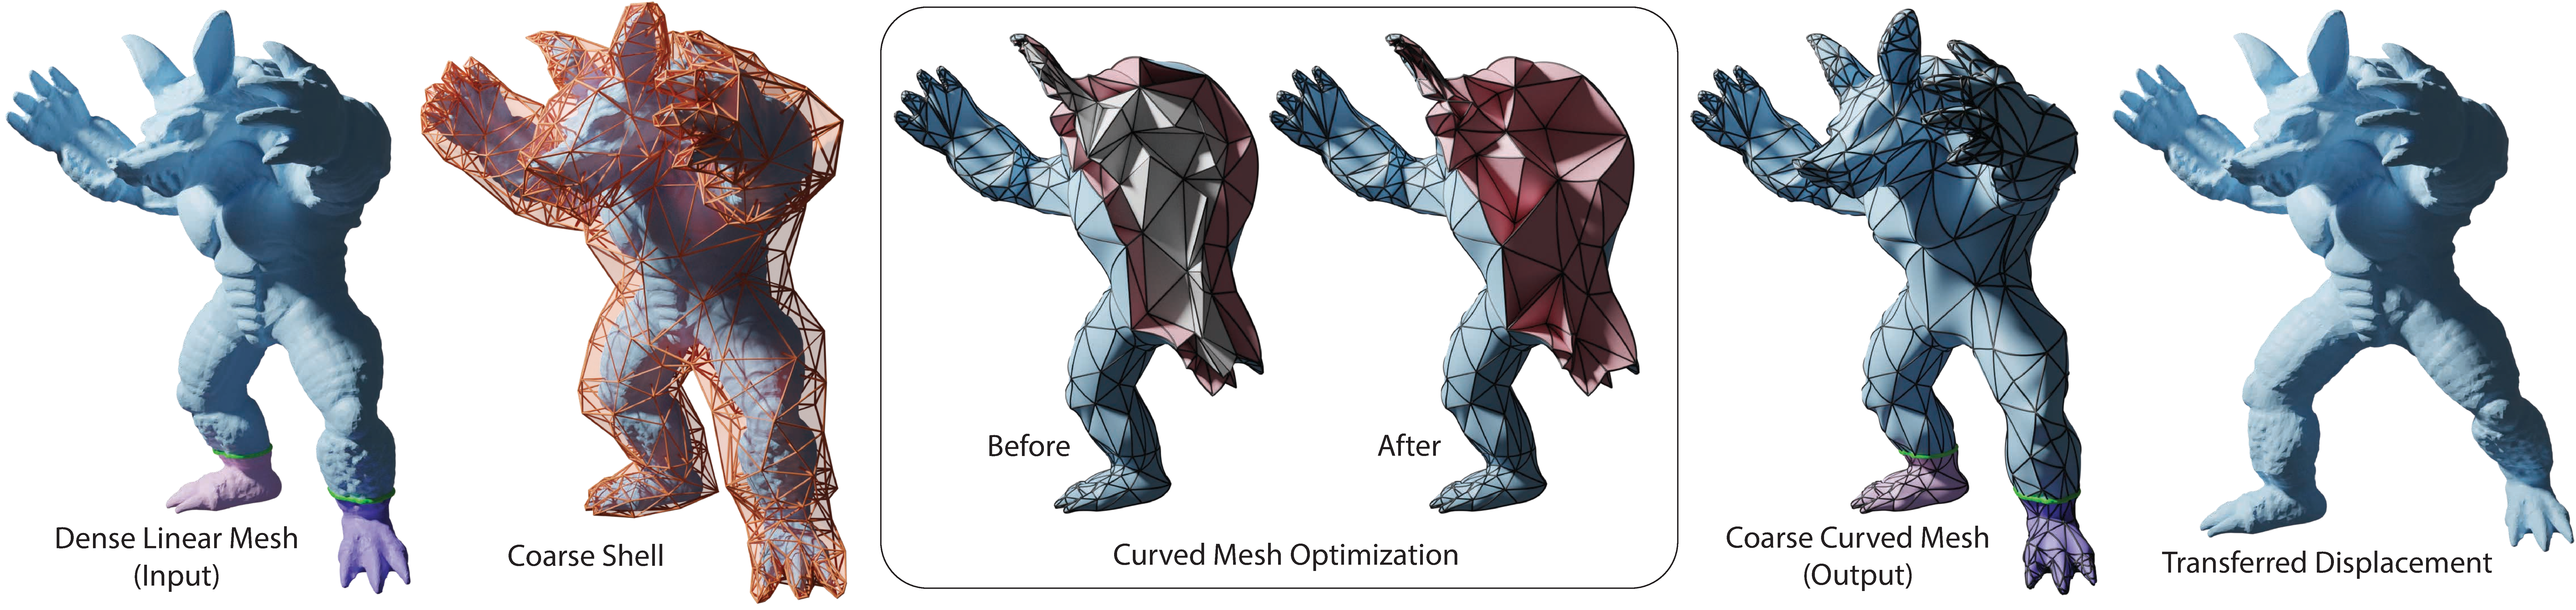
\includegraphics[width=\linewidth]{curve_meshing_in_shell_tex/figs/teaser}
\caption{Our pipeline starts from a dense \emph{linear} mesh with annotated features (green), which is converted in a curved shell filled with a high-order mesh. The region bounded by the shell is then tetrahedralized with linear elements, which are then optimized. Our output is a coarse, yet accurate, curved tetrahedral mesh ready to be used in FEM based simulation. Our construction provides a bijective map between the input surface and the boundary of the output tetrahedral mesh, which can be used to transfer attributes and boundary conditions.}
\label{bichon:fig:teaser}
\end{teaserfigure}

\maketitle


\begin{figure}
    \centering
    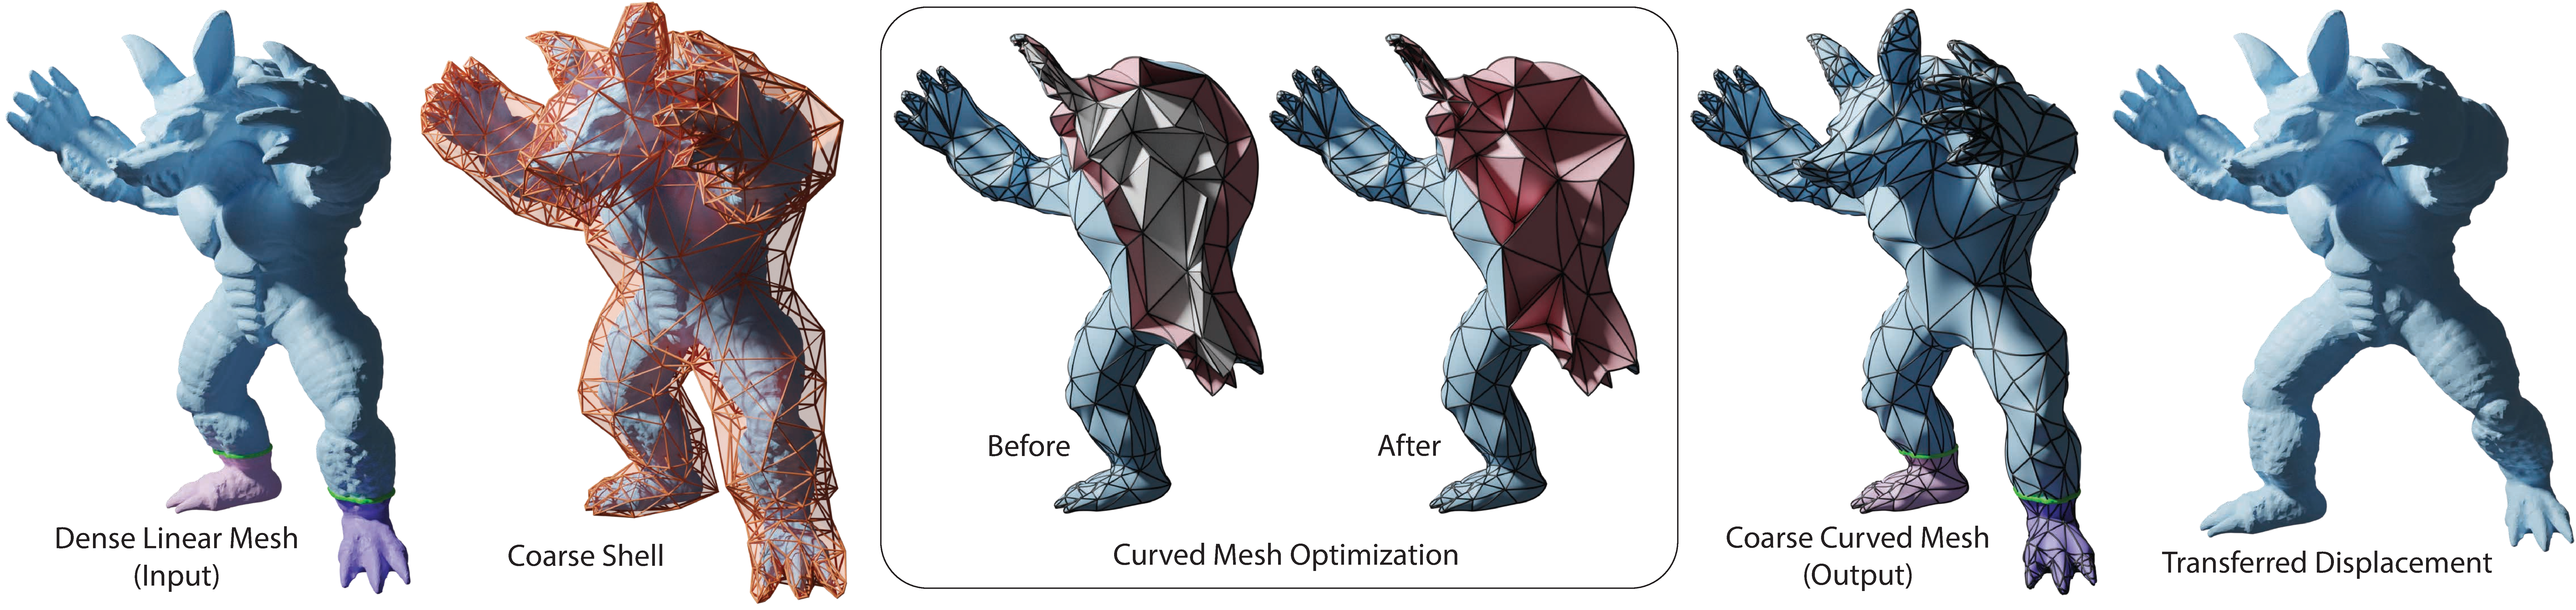
\includegraphics[width=\linewidth]{curve_meshing_in_shell_tex/figs/teaser}
    \caption{Our pipeline starts from a dense \emph{linear} mesh with annotated features (green), 
    which is converted in a curved shell filled with a high-order mesh. The region bounded by the shell is then tetrahedralized with linear elements, which are then optimized. Our output is a coarse, yet accurate, curved tetrahedral mesh ready to be used in FEM based simulation. Our construction provides a bijective map between the input surface and the boundary of the output tetrahedral mesh, which can be used to transfer attributes and boundary conditions.}
    \label{bichon:fig:teaser}
\end{figure}

\section{Introduction}

Piecewise linear approximations of surfaces are a popular representation for 3D geometry due to their simplicity and wide availability of libraries and algorithms to process them. However, dense sampling is required to faithfully approximate smooth surfaces. 
%
Curved meshes, that is, meshes whose element's geometry is described as a high-order polynomial, are an attractive alternative for many applications, as they require fewer elements to achieve the same representation accuracy of linear meshes. In particular, curved meshes have been shown to be effective in a variety of simulation settings in mechanical engineering, computational fluid dynamics, and graphics. Despite their major benefits, they are not as popular as linear meshes: We believe that {one of} the main reason for their limited usage is the lack of an automatic, robust way of constructing them. 

While robust meshing algorithm exists for volumetric linear tetrahedral meshing, there are few algorithms for curved meshes, and even fewer of them having either a commercial or open-source implementation (Section \ref{sec:related}). Only {a} few algorithms work directly on arbitrary triangle meshes (most of them require the input geometry to be either a CAD file or an implicit function), and none of them can reliably process a large collection of 3D models. 

We propose the first robust and automatic algorithm to convert dense piecewise linear triangle meshes (which can be extracted from scanned data, volumetric imaging, or CAD models) into coarse, curved tetrahedral meshes equipped with a bijective map between the input triangle mesh and the boundary of the tetrahedral mesh. Our algorithm takes advantage of the recently proposed bijective shell construction \cite{jiang2020bijective} to allow joint coarsening, remeshing, and curving of the dense input mesh, which we extend to support feature annotations.
Our outputs are guaranteed to have a self-intersection free boundary and the geometric map of every element is guaranteed to be bijective, an important requirement for FEM applications.

The key ingredient of our algorithm is the separation of the curved volumetric meshing problem into a near-surface, surface curving problem, followed by a restricted type of linear volumetric meshing. 

% This is repetitive
%For the former, we use prismatic elements to create a valid parametrization close to the surface, and use it to ensure validity during mesh coarsening and curving.

% \TS{i dont think we should state this here}
% An important subproblem, of independent interest, that we tackle in this paper is constrained linear volumetric meshing (i.e. fill the interior of closed, non self-intersecting triangle mesh without refining it), for which we propose a simple and robust algorithm that is inspired by the TetWild algorithm \cite{hu2018tetrahedral}.

We believe that our curved meshing algorithm will enable wider adoption of curved meshes, as it will provide a way to automatically convert geometric data in multiple formats into a coarse tetrahedral mesh readily usable in finite element applications. To showcase the benefits of our approach we study 2 settings: (1) we show that a coarse proxy mesh can be used to compute non-linear deformations efficiently and transfer them onto a high-resolution geometry, targeting real-time simulation (Figure~\ref{bichon:fig:teaser}), and (2) 
we show that our meshes are ready to use in downstream FEM simulations.

% Additionally, we show that the boundary of our tetrahedral mesh, which is a curved (yet only $C^0$) surface mesh is useful for automatically generating assets for real-time rendering pipelines, despite the lack of normal continuity across patches.
% \DP{Or maybe not? Let's see.}

We validate the reference implementation of our approach on a large collection of more than 8000 geometrical models, which will be released as an open-source project to foster the adoption of curved meshes in academia and industry.

Our contributions are:
\begin{itemize}
    \item An algorithm to convert dense piecewise linear meshes into coarse curved volumetric meshes while preserving a bijective map with the input and bounding the approximation error.
    \item An extension of the bijective shell construction algorithm to support feature {annotations}.
    \item An algorithm for conforming tetrahedral meshing without allowing refinement on the boundary, but allowing internal Steiner points.
    % \item A reusable open-source implementation of our algorithm evaluated on a large scale benchmark.
    \item A large-scale dataset of high-order tetrahedral meshes.
\end{itemize}
\section{Related Works}\label{cumin:sec:related}

We review the literature on the generation of unstructured and structured curved meshes. We also review the literature on boundary-preserving linear meshing, as it is an intermediate step of our algorithm.

\subsection{Curved Tetrahedral Mesh Generation}

High-order meshes are used in applications in graphics \cite{bargteil2014animation,MEZGER2009680,Suwelack2013} and engineering analysis \cite{Jameson2002} where it is important to reduce the geometric discretization error \cite{Babuska1988,BABUSKA1992159,BASSI1997251,luo2001influence,ODEN1994309}, while using a low number of degrees of freedom. The creation of high-order meshes is typically divided into three steps: (1) linear meshing of the smooth input surface, (2) curving of the linear elements to fit the surface, and (3) optimization to heal the elements inverted during curving. We first cover steps 2 and 3, and postpone the overview of linear tetrahedral algorithms to Section \ref{cumin:sec:rel:linear}.

\paragraph{Direct methods.} Direct methods are the simplest family of curving algorithms, as they explicitly interpolate a few points of the target curved surface or project the high-order nodes on the curved boundary  \cite{dey1999curvilinear,Ghasemi2016,MOXEY2015636,abgrall2012,sherwin2002mesh,turner2017high,marcon2019semi}. The curved elements are represented using Lagrange polynomials, \cite{dey1999curvilinear,Peir2008}, quadratic or cubic B{\'e}zier polynomials \cite{George2012,Qiukai2013,Luo2002pVersionMG}, or NURBS \cite{ENGVALL2016378,ENGVALL201783}. \cite{SHEPHARD2005251,sherwin2002mesh} further optimizes the high-order node distribution according to geometric quantities of interest, such as length, geodesic distance, and curvature. 
In the case where no CAD information is available, \cite{wang2016construction}, \cite{jiao2012reconstructing} use smooth reconstruction to compute high-order nodes and perform curving.

\paragraph{Deformation methods} Deformation methods consider the input linear mesh as a deformable, elastic body, and use controlled forces to deform it to fit the curved boundary. Different physical models have been employed such as linear, \cite{Abgrall2014,abgrall2012,dobrzynski2017,Xie2013}, and (variants of) non-linear elasticity \cite{Persson2009,MOXEY2016130,FORTUNATO20161}. A comparison between different elasticity and distortion energies is presented in \cite{Poya2016, TURNER2016340, dobrev2019target}.

Direct and deformation methods have been tested on small collections of simple models, and, to the best of our knowledge, none of them can provide guarantees on the validity of the output or has been tested on large collections of models. There are also no  reference implementations we could compare against. 

\paragraph{Inversions and Intersections.} Most of these methods introduce inverted elements during the curving of the high-order elements. Inverted elements can be identified by extending Jacobian metrics for linear elements \cite{Knupp20002,Knupp2000} to high-order ones \cite{Luke2018,Gargallo2014,johnen2013geometrical,Poya2016,Roca2012}. Various untangling strategies have been proposed, including geometric smoothing and connectivity modifications  \cite{Cardoze2004,dey1999curvilinear,gargallo2013high,George2012,Qiukai2013,Luo2002pVersionMG,Peir2008,SHEPHARD2005251,dobrzynski2017,Gargallo2015,Geuzaine2015,Roca2012,RUIZGIRONES2017362,RUIZGIRONES201652,RUIZGIRONES2016315,STEES2017180,Steve2016,TOULORGE20138,TOULORGE2016361,ZIEL201791,dobrev2019target, turner2017high, luo2008tracking,lu2014parallel}.  None of these techniques can guarantee to remove the inverted elements.

An alternative approach is to start from an inversion-free mesh and slowly deform it \cite{Persson2009,RUIZGIRONES2017362}, explicitly avoiding inversions at the cost of possibly inaccurate boundary reproductions. These methods cannot however guarantee that the boundary will not self-intersect. Our approach follows a similar approach but uses a geometric shell to ensure element validity and prevention of boundary self-intersections.

\paragraph{Curved Optimal Delaunay Triangulation}
\cite{feng2018curved} generalize optimal delaunay triangulation paradigm to the high-order setting, through iteratively update vertices and connectivity.
Their algorithm starts with a point cloud sampled from triangle meshes. However, the success of the method depends on the choice of final vertex number and sizing field, where insufficient vertices may result in broken topology or invalid tetrahedral meshes.

\paragraph{Software Implementation.}
Despite the large literature on curve{d} meshing generation, there are very few implementations available. 

Nektar~\cite{moxeynekmesh} is a finite element software with a meshing component, which can generate high-order elements. We do not explicitly compare as their documentation (Section 4.5.1.5 Mesh Correction\footnote{\url{https://doc.nektar.info/userguide/5.0.0/user-guidese17.html}}) states that the algorithm is not fully automatic and not designed to process robustly large collections of models.
Gmsh~\cite{Geuzaine:2009:gmsh} is an open source software that supports the curved meshing of CAD models, but it does not support dense linear meshes as input. Despite the difference in the input type, we provide a comparison with Gmsh in Section \ref{cumin:sec:comparison}, as it is the only method that we could run on a large collection of shapes.

To the best of our knowledge, the commercial software that support curved meshing (Pointwise \cite{pointwise,Steve2016}) are also requiring a CAD model as input.

\paragraph{Animation}
Curved tetrahedral meshes have also gained popularity in the context of fast animation. With fewer degrees of freedom and preserved geometric fidelity, 
\cite{mezger2007finite} observe the benefit of quadratic tetrahedra in the pipeline of physically based animation.
\cite{Suwelack2013} further investigate the transfer problem when using curved meshes as a proxy.

\subsection{Curved Structured Mesh Generation}

The use of a hexahedral mesh as a discretization for a volume, allows to naturally define $C^k$ splines over the domain, which can be used as basis functions for finite element methods: this idea has been pioneered by 
IsoGeometric Analyisis (IGA), and it is an active research area. The generation of volumetric, high-order parametrizations that conform to a given input geometry is an extremely challenging problem \cite{Sorger:2014,Peir2015OnCH}. Most of the existing methods rely on linear hexahedral mesh generation, which is on its own a really hard problem for which automatic and robust solutions to generate coarse meshes are still elusive \cite{Yufei:2012,Gao:2019,Guo2020Cut,Palmer:2020,Zhang:2020,marschner2020hexahedral} due to the inherently global nature of the problem. 
%
The current state of the art for IGA meshing is a combination of manual decomposition of the volume and semi-automated geometrical fitting \cite{yu2020hexgen,coreform}.

In contrast, our approach is automatic, i.e. can automatically process thousands of models without any manual intervention, while providing explicit guarantees on both the validity of the elements and the maximal geometric error. Its downside is the $C^0$ continuity of the basis on the elements' interfaces. However, it is unclear to us if this is a real limitation: in many common settings in computer graphics and mechanical engineering (Poisson problems, linear and non-linear elasticity) the higher smoothness offered by spline functions does not make noticeable difference experimentally \cite{schneider2019large} (and it actually leads to much worse conditioning of the system matrix, which is problematic for iterative solvers), and we thus believe that curved tetrahedral meshing is a very exciting alternative as it dramatically simplifies both the meshing and fitting of high-order elements.

\subsection{Boundary Preserving Tetrahedral Meshing}
\label{cumin:sec:rel:linear}

We refer to \cite{hu2018tetrahedral} for a detailed overview of linear tetrahedral meshing, and we focus here only on the techniques that target boundary preserving tetrahedral meshing. 

The most popular linear tetrahedral meshing methods are based on {\em Delaunay refinement}
\cite{chew1993guaranteed,shewchuk1998tetrahedral,ruppert1995delaunay}, i.e. the insertion of new vertices at the center of the circumscribed sphere of the worst
tetrahedron in term of radius-to-edge ratio. This approach is used in the most popular tetrahedral meshing implementations  \cite{tetgen,jamin2015cgalmesh}, and, in
our experiments, proved to be consistently successful as long as the boundary is allowed to be refined. A downside of these approaches is that a 3D Delaunay mesh, unlike the 2D case, might still contain ``sliver'' tetrahedra, thus requiring mesh improvement
heuristics \cite{cheng2000silver,du2003tetrahedral,alliez2005variational,tournois2009interleaving}. \cite{Alexa:2019} discusses this issue in detail and provides a different formulation to avoid it without the use of a postprocessing. 
%
\cite{alexa2020conforming} introduces an approach that does not allow insertion of Steiner points, making it not suitable for generic polyhedra domains.

There are many variants of {Delaunay-based} meshing algorithms including 
{\em Conforming Delaunay tetrahedralization}
\cite{murphy2001point,CohenSteiner:2002:CDT}, {\em constrained Delaunay tetrahedralization}
\cite{chew1989constrained,si2005meshing,shewchuk2002constrained,SiS14}, and {\em Restricted Delaunay tetrahedralization}\ \cite{cheng2008practical,boissonnat2005provably,Engwirda16}.

To the best of our knowledge, all these methods are designed to allow some modifications of the input surface (either refinement, resampling, or approximation). One exception is the constrained Delaunay implementation in TetGen \cite{tetgen} that allows disabling any modification to the boundary. However, this comes at the cost of much lower quality and potential robustness issues, as we show in Appendix \ref{app:tetgen}. 

A different tetrahedral meshing approach has been proposed in \cite{hu2018tetrahedral}, and its variants \cite{Hu:2020:fTetWild,hu2019triwild}, where the problem is relaxed to generate a mesh that is close to the input to increase robustness. However, these approaches are not directly usable in our setting, as we require boundary preservation.

Due to these issues, we propose a novel boundary-preserving tetrahedral meshing algorithm specifically tailored for the shell mesh generated by our curved meshing algorithm.

\subsection{Curved Surface Fitting}
There are many algorithms for fitting curved \emph{surfaces} to dense 3D triangle meshes. The most popular approaches fit spline patches, usually on top of a quadrangular grid. Since generating quadrilateral meshes is a challenging problem for which robust solutions do not exist yet, we refer to \cite{QUADSTAR2012} for an overview, and only review in this section algorithms for unstructured curve{d} mesh generation, which are more similar to our algorithm. We note that the focus of our paper is volumetric meshing: while we generate an intermediate curved surface mesh, this is not the goal of our algorithm, especially since the generated surface is only $C^0$ on edges.

\cite{hoppe1994piecewise} fits a smooth surface represented by a point cloud to a curved triangle mesh based on a subdivision surface scheme and an interleaving mesh simplification and fitting pipeline that preserves sharp features. 
The algorithm does not provide explicit correspondence to the input: they are defined using distance closest point, which is not bijective far from the surface. 

\cite{krishnamurthy1996fitting} converts dense irregular polygon meshes of arbitrary topology into coarse tensor product B-spline surface patches with accompanying displacement maps. Based on the work \cite{LIN2007adap} that fits triangle surface meshes with B\'ezier patches, \cite{Zhang2011multi} fits triangle surface meshes with high-order B-spline quadrilateral patches and adaptively subdivide the patches to reduce the fitting error. These methods produce smooth surfaces but do not have feature preservation.

Another related topic is the definition of smooth parametric surfaces interpolating triangle meshes. We refer to \cite{zorin2000subdivision} for an overview of subdivision methods and discuss here the approaches closer to our contribution.

\cite{Hahmann2003} proposed to use triangular B\'ezier patches to define smooth surfaces over arbitrary triangle meshes ensuring tangent plane continuity by relaxing the constraint of the first derivatives at the input vertices.
%
Following Hahmann's work, \cite{yvart2005smooth} presents a more complete pipeline: perform QEM simplifications, trace the coarse mesh onto the dense one and perform parameterization relaxing and smoothing. Then it fits a hierarchical triangular spline~\cite{Yvart2005hier} to the surface.
%
More recent work \cite{TONG2009} approximates the triangulation of an implicit surface with a $G^1$ surface.
%
These schemes are usually designed to interpolate existing meshes rather than simplifying a dense linear mesh into a coarse curved mesh and are thus orthogonal to our contribution.

% \cite{losasso2003smooth} Smooth geometry images. quad mesh?

% \url{https://www.graphics.rwth-aachen.de/media/papers/campen_siggraph2017_Similarity-T-Splines.pdf}

% \TODO{better to change gmsh paper to: The Generation of Valid Curvilinear Meshes}


\subsection{Variation from the Original Algorithm}
To extend the shell formulation in~\ref{chp:shell} to accommodate for feature preservation (Section \ref{cumin:sec:features-pres}), 
we modify the definition of a valid section (Chapter~\ref{chp:shell} Definition 3.1), 
by relaxing the intersection between a triangle and a prism in the discrete case. That is, we do not consider the prism to be intersecting a triangle if they share only one vertex of the triangle; we also ignore the intersection if they intersect on a feature edge on opposite sides. The bijectivity and validity condition of the shell projection trivially holds.

%%%%%%%%%%%%%%%%%%%%%%%%%%%%%%%%%%%%%%%%%%%
%%%%%%%%%%%%%%%%%%%%%%%%%%%%%%%%%%%%%%%%%%%

\begin{figure}
    \centering
    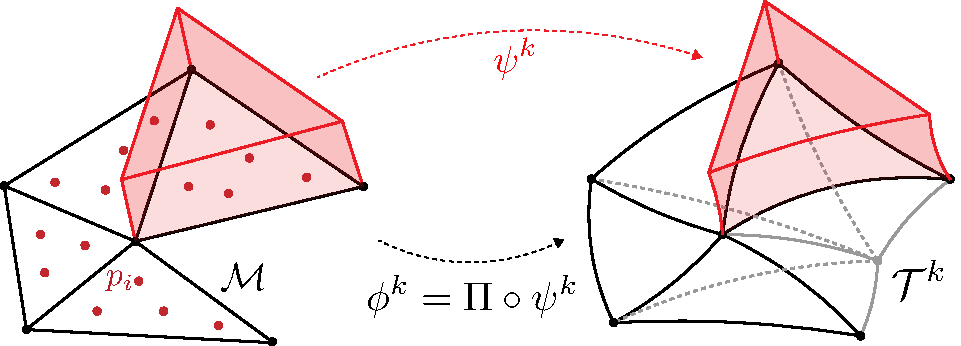
\includegraphics[width=.8\linewidth]{curve_meshing_in_shell_tex/figs/illustrations/input-output.pdf}
    \caption{Input triangle mesh $\M$ and points $\P$. Output curved tetrahedral mesh $\T^k$ and bijective map $\phi^k$.}
    \label{bichon:fig:input-output}
\end{figure}

\section{Curved Tetrahedral Mesh Generation}\label{cumin:sec:curved-pipeline}



\paragraph{Input.}
The input of our algorithm is a collection of oriented manifold, watertight, self-intersection-free triangle mesh $\M=(V,F)$, and a set of points $p_i\in\P$ (possibly empty) on the surface of $\M$ (Figure~\ref{bichon:fig:input-output}, left) where the distance bound $\varepsilon$ is prescribed. The collection $\M$ must be consistently oriented such that it is the boundary of an oriented 3-manifold.
A set of edges can also be optionally provided as annotated features (Section~\ref{cumin:sec:features-pres}).

\begin{figure}
    \centering
    % \includegraphics[width=.6\linewidth]{curve_meshing_in_shell_tex/figs/nodes}\hfill
    % \includegraphics[width=.37\linewidth]{curve_meshing_in_shell_tex/figs/gmapping}
    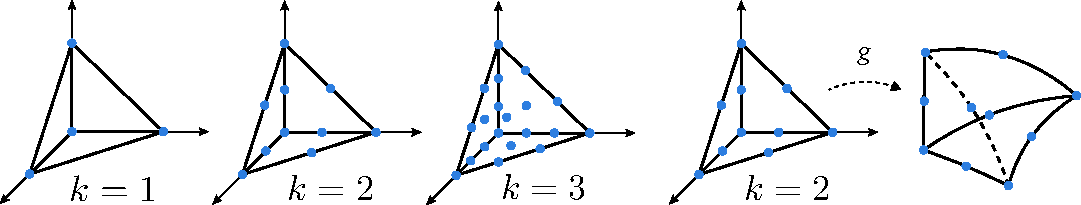
\includegraphics[width=\linewidth]{curve_meshing_in_shell_tex/figs/illustrations/high-order.pdf}
    \caption{Lagrange nodes on the reference element $\hat \tau$ for different $k=1,2,3$, and example of geometric mapping $g$.}
    \label{bichon:fig:high-order}
\end{figure}

\paragraph{Output.}
The output of our algorithm is a tetrahedral mesh $\T^k = (V^k,T^k)$ of order $k$. 
Formally, each tetrahedron $\tau\in T^k$ is defined through the \emph{geometric map} from the reference tetrahedron $\hat \tau$,
\begin{equation}\label{eq:gmap}
g^\tau = \sum_{j=1}^n c_j^\tau L_j(\hat u,\hat v,\hat w),
\end{equation}
where $\hat u,\hat v,\hat w$ are the local coordinates of a point in $\hat \tau$, $c_j^\tau$ are the control points for a tetrahedron $\tau$, and $L_j$ are polynomial bases (typically Lagrange bases).
For two tetrahedra $\tau_1$ and $\tau_2$ 
of $T^k$ sharing a face $F$, the restriction of the maps $g^{\tau_i}$, $i=1,2$, to $F$ coincide.
Figure~\ref{bichon:fig:high-order} shows the position of the control points $c_j$ on the reference element for $k=1,2,3$ for the Lagrange bases. We call the tetrahedralization of a curved mesh $\T^k$ \emph{positive} if $\det(J_{g^\tau}) > 0$ everywhere on every $\tau$. 
% That is, we require that the geometric mapping $g^T$ is bijective for every tetrahedron \DP{I don't think this is true, the implication holds the other way, discuss.} \DZ{Indeed this is obviously not true except in the linear case; positive Jacobian only guarantees local injectivity; a sufficient condition is that the map is bijective on the boundary}. 
In particular, for $k=1$, since $g$ is affine, $J_{g^\tau}$ is constant and the positivity reduces to the positive orientation of the vertices \cite{shewchuk1997adaptive}.

Note that, while bijectivity of the geometric map $g^\tau$ implies positivity, the reverse is not true. 
Therefore, our algorithm not only checks for $\det(J_{g^\tau}) > 0$, but also ensures that the boundary $\partial\T^k$ does not intersect; we show in section~\ref{cumin:sec:bij-proof} that these two conditions guarantee the bijectivity of $g^\tau$.
Furthermore, our algorithm ensures that the distance from any point in $\P$ to $\partial\T^k$ (the surface of $\T^k$) is smaller than an user-controlled parameter $\varepsilon$.

\begin{figure}
    \centering\small
    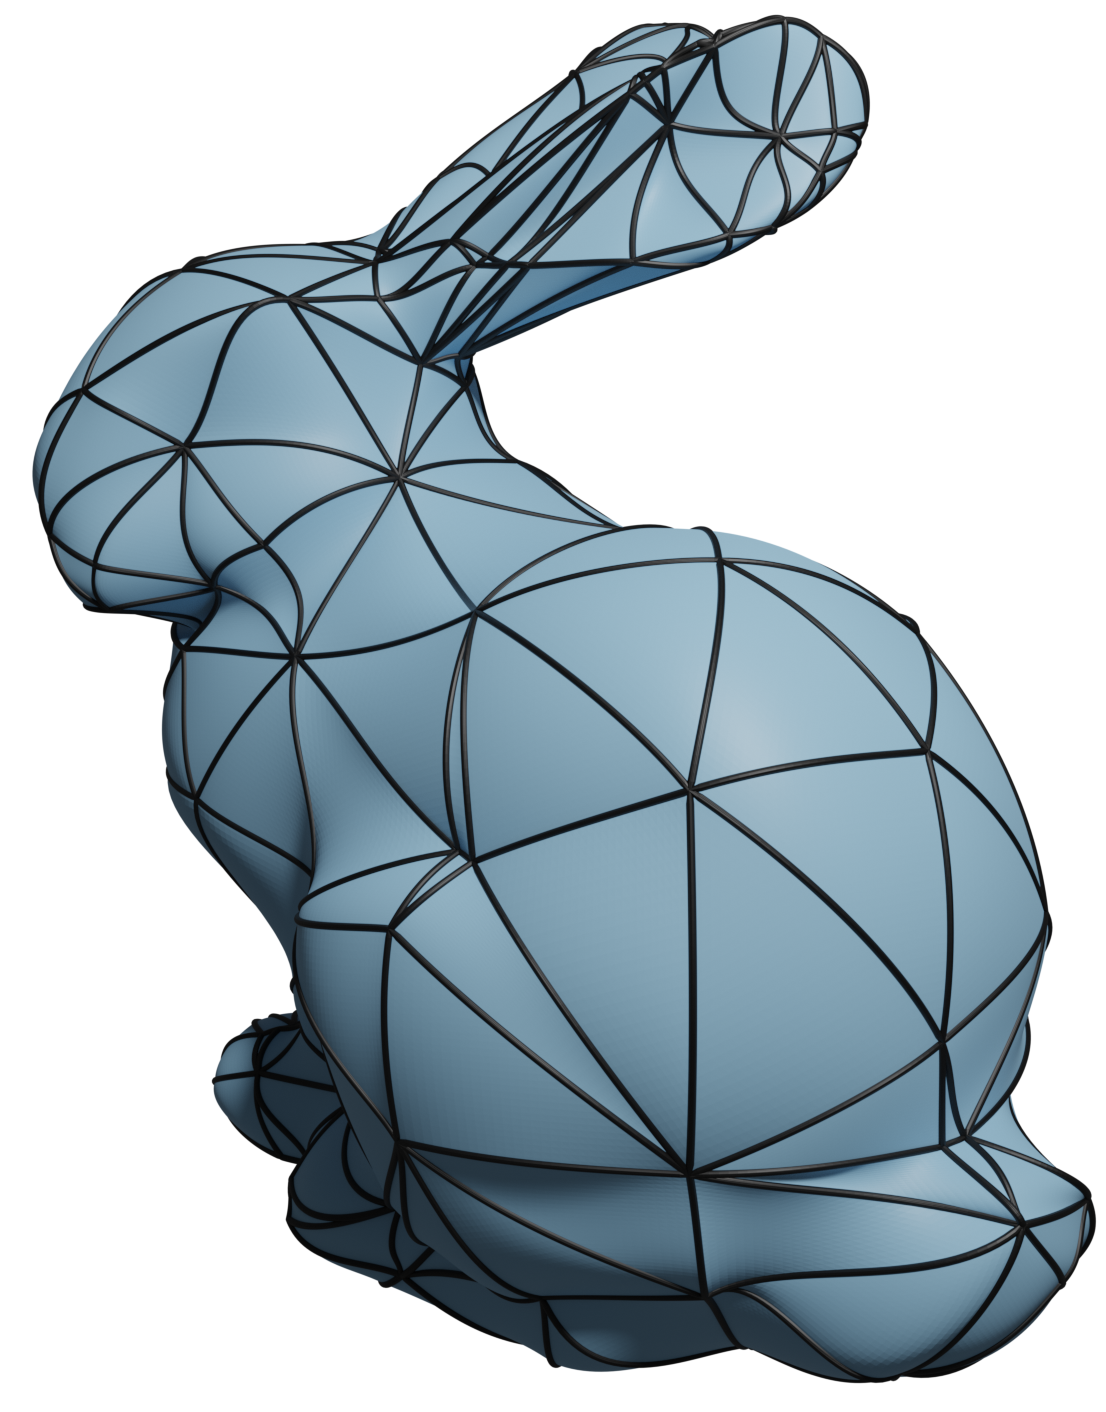
\includegraphics[width=0.23\linewidth]{curve_meshing_in_shell_tex/figs/bunny/0001}\hfill
    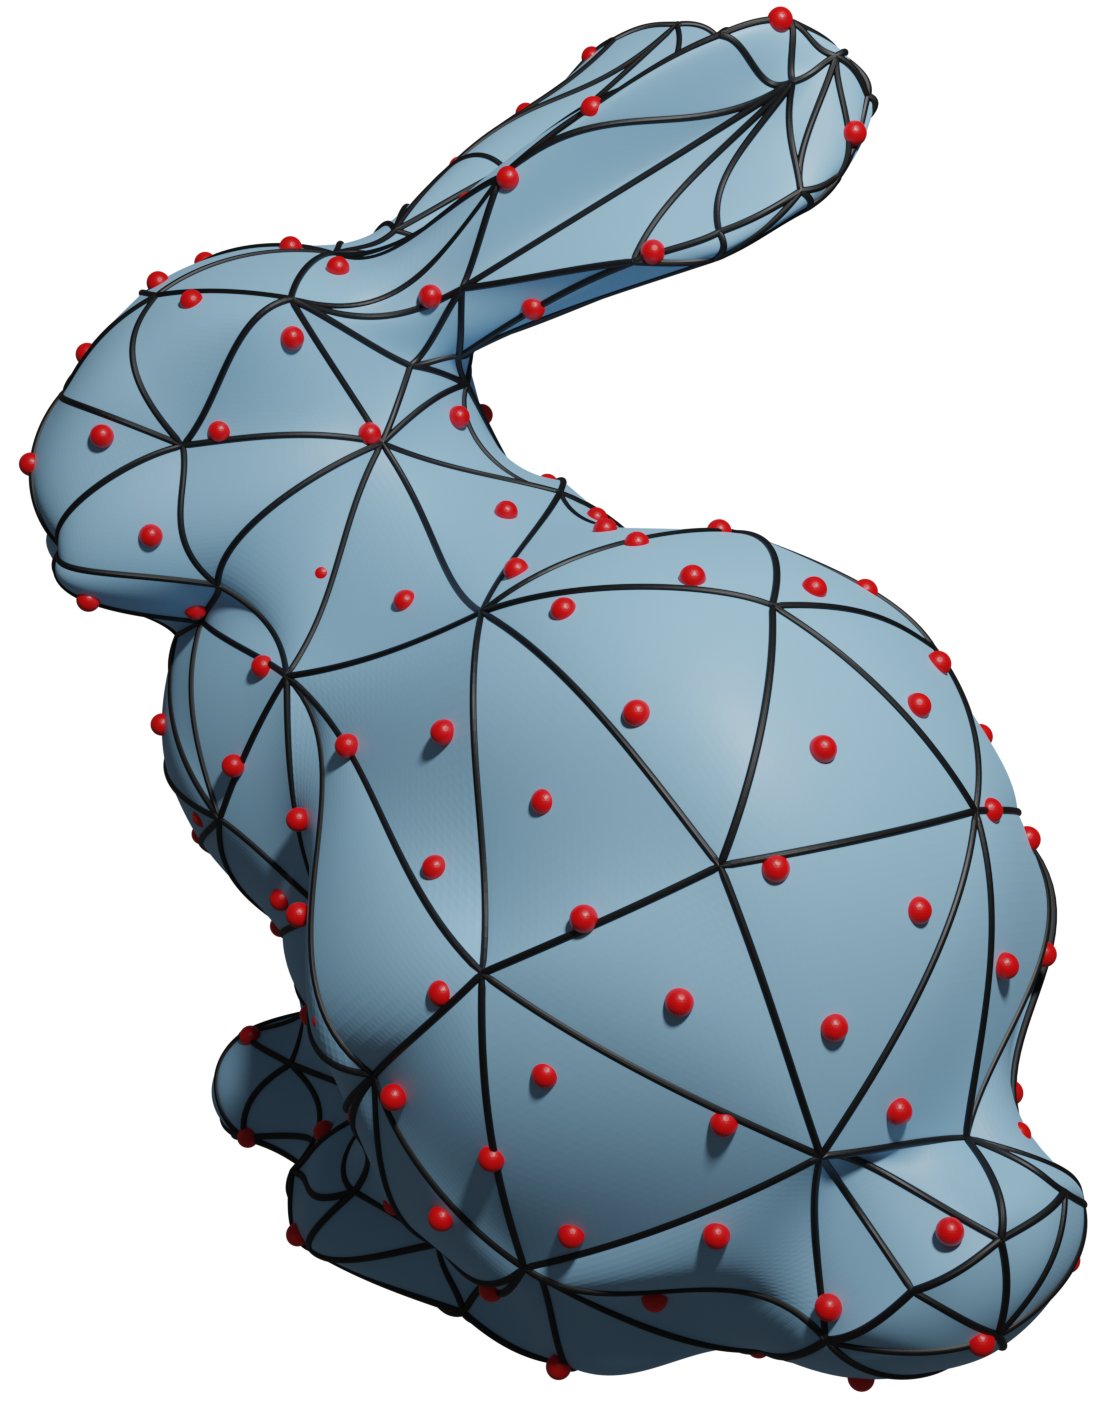
\includegraphics[width=0.23\linewidth]{curve_meshing_in_shell_tex/figs/bunny/0004}\hfill
    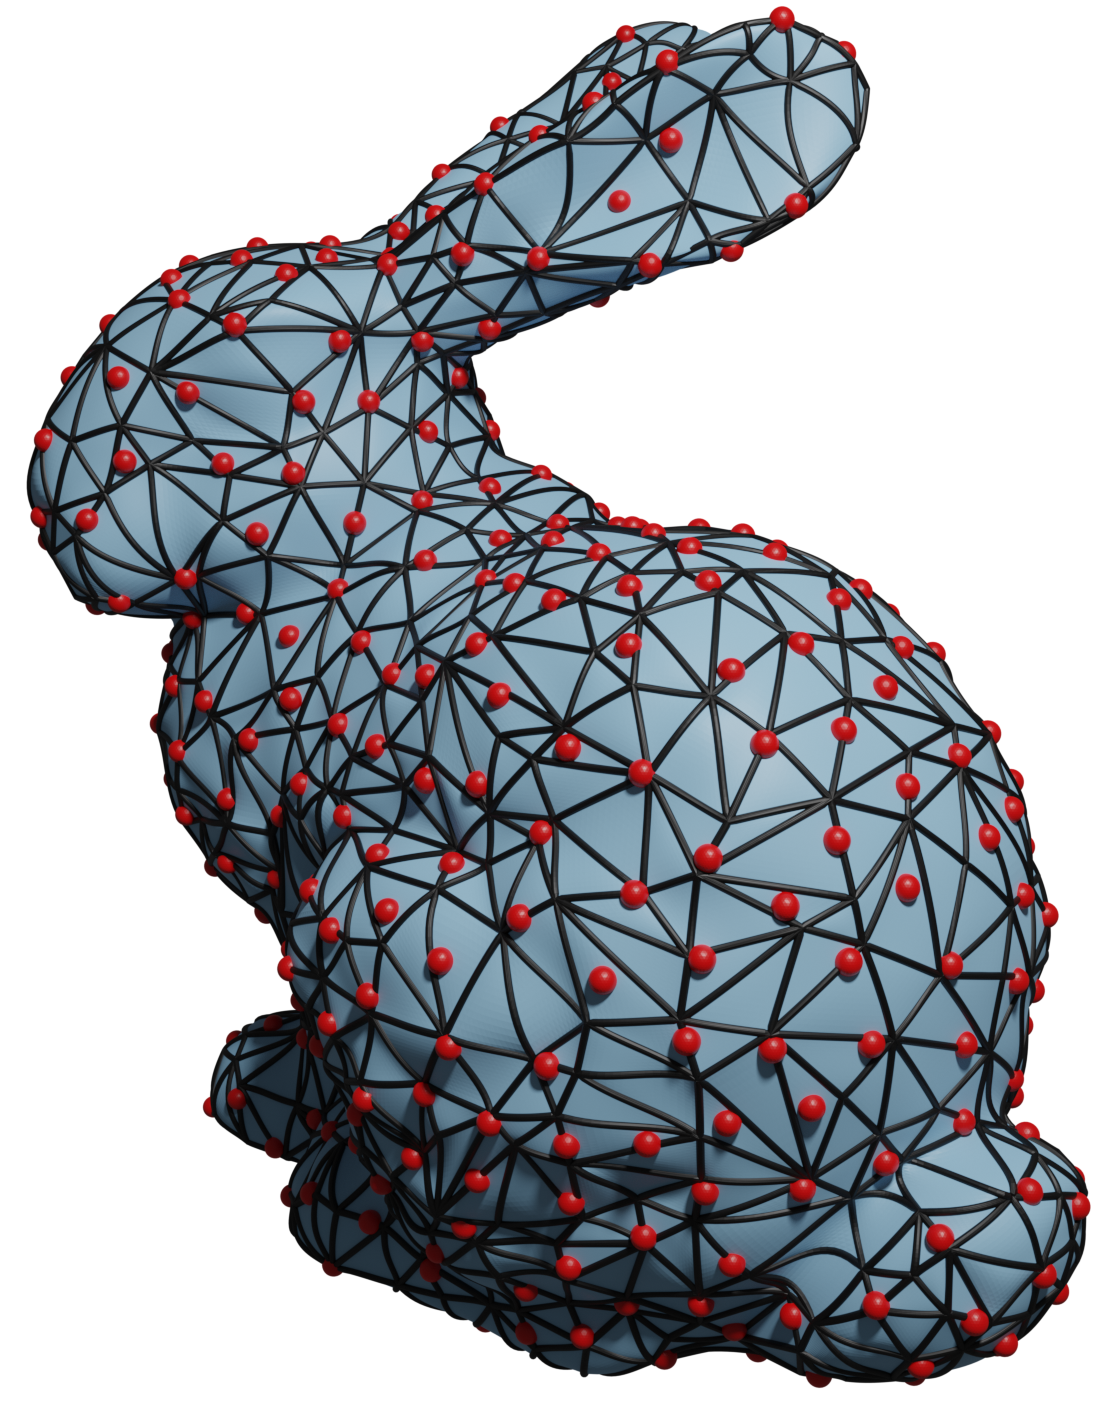
\includegraphics[width=0.23\linewidth]{curve_meshing_in_shell_tex/figs/bunny/0003}\hfill
    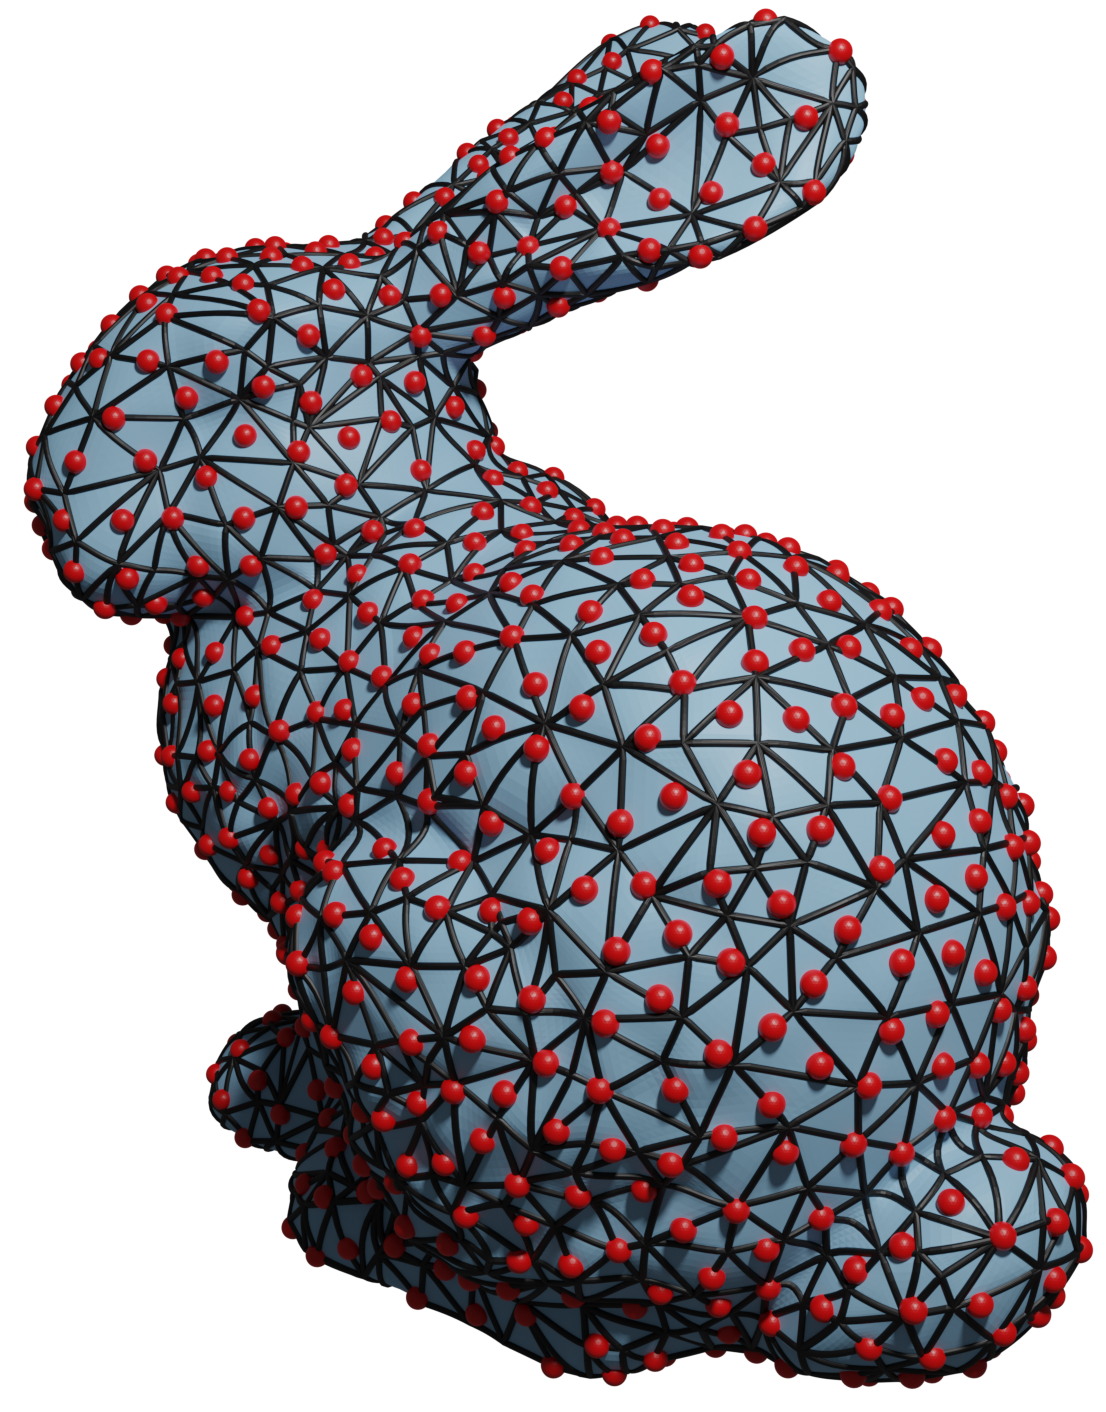
\includegraphics[width=0.23\linewidth]{curve_meshing_in_shell_tex/figs/bunny/0002}\par
    \parbox{.23\linewidth}{\centering 0 points.}\hfill
    \parbox{.23\linewidth}{\centering 200 points.}\hfill
    \parbox{.23\linewidth}{\centering 500 points.}\hfill
    \parbox{.23\linewidth}{\centering 1000 points.}
    \caption{Effect of the choice of the set $\P$ on the output.}
    \label{bichon:fig:points-effect}
\end{figure}



We are not assuming anything on $\P$: a sparse set of points will generate a mesh less faithful to the input geometry, while a dense sampling computed for instance with Poisson disk sampling~\cite{bowers2010parallel} will prevent the surface from deviating too much (Figure~\ref{bichon:fig:points-effect}).


Our algorithm guarantees that the tetrahedralization is positive and that $\partial\T^k$ does not have self-intersections. 
It also aims at coarsening {$\T^k$} as much as possible while striving to obtain a good geometric quality. 
To reliable fit $\partial \T^k$ to $\M$ we require a bijective map
\[
\phi^k \colon \M \to \partial \T^k
\]
from the input $\M$ to the surface of $\T^k$ (Figure~\ref{bichon:fig:input-output} right). Our algorithm also generates this map and exposes it as an output for additional uses, such as attribute transfer. Note that, since we build upon the shell construction in~\ref{chp:shell}, we also {guarantee} $\partial\T^k$ is homeomorphic and topology-preserving with respect to $\M$ (Figure~\ref{bichon:fig:intersection}).


\begin{figure}
    \centering
    % \includegraphics{}
    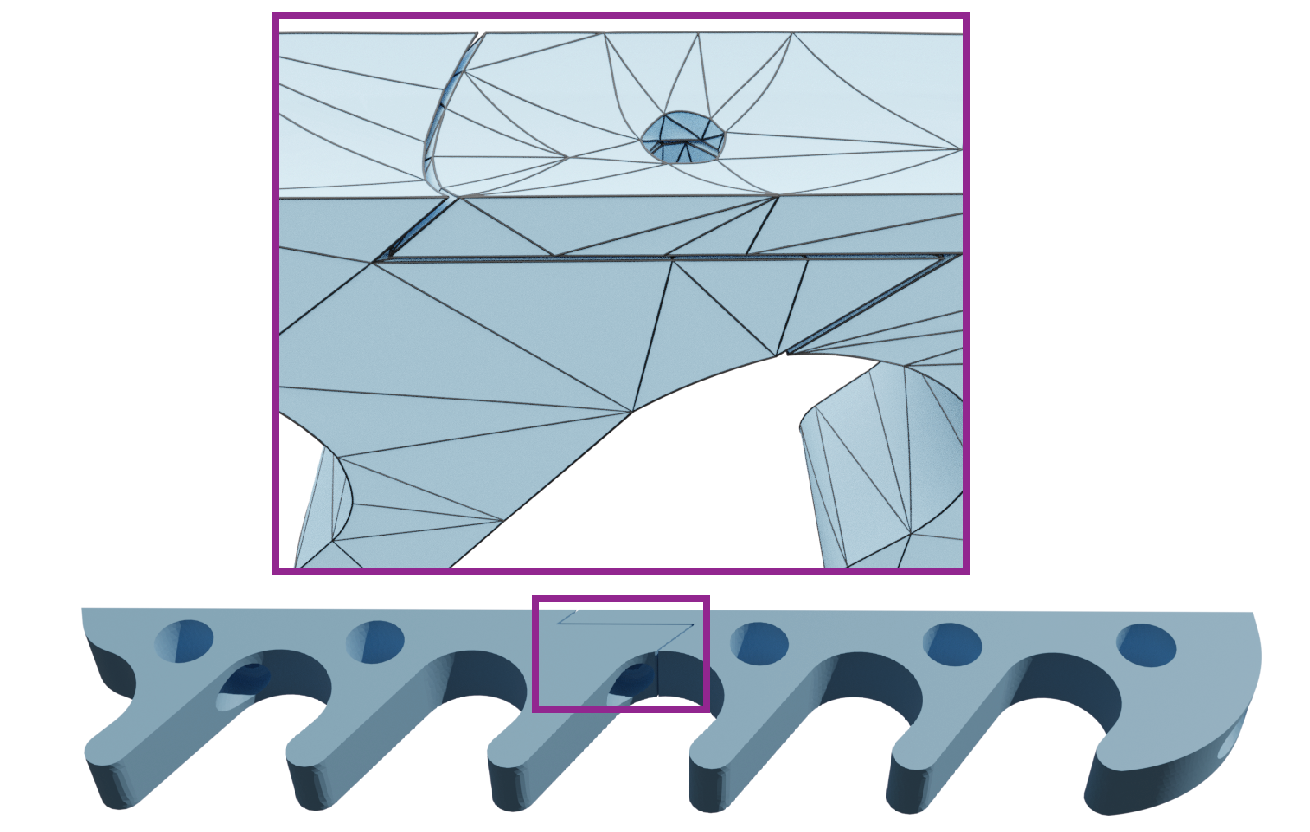
\includegraphics[width=0.9\linewidth]{curve_meshing_in_shell_tex/figs/intersection-free.pdf}\hfill
    \caption{Our algorithm maintains {free of} intersection even on challenging models, without the need of setting adaptive threshold.}
    \label{bichon:fig:intersection}
\end{figure}


%For each edge provided in the feature annotation list, 
%there exists one curved edge in the output mesh, 
%where the marked edge is in bijective correspondence to a segment in the curved edge.


To simplify the explanation{,} we use the bar $\overline{\phantom{M}}$ to represent quantities on the \emph{straight} linear shell, the tilde $\widetilde{\phantom{M}}$ for the \emph{curved} shell, and hat $\hat{\phantom{M}}$ for the reference elements (e.g., $\overline P$ is the prism on {the} straight coarse shell, $\widetilde P$ is the curved prism, and $\hat P$ is the prism on the reference configuration).


\begin{definition}\label{def:curved-mesh}
We call a curved mesh $\T^k$ and its mapping $\phi^k$ to $\M$ \emph{valid} if it satisfies the following conditions:
\begin{enumerate}
    \item $\phi^k$ is bijective;
    \item the distance between any $p\in\P$ and $\partial\T^k$ is less than $\varepsilon$;
    \item $\T^k$ is positive (i.e., every geometric map $g^\tau$ has positive Jacobian's determinant).
\end{enumerate}
\end{definition}

\paragraph{Overview.} 
Our algorithm starts by creating a valid mesh (i.e., it satisfies~\ref{def:curved-mesh}), then it performs local operations (section~\ref{app:local-ops}) to improve $\T^k$ (i.e., coarsen it and improve its quality) while ensuring all the conditions remain valid with respect to local modification. 
To achieve this goal, our algorithm uses two stages: (1) curved shell generation and (2) tetrahedral mesh generation and optimization.

\begin{figure}
    \centering
    \includegraphics[width=\linewidth]{curve_meshing_in_shell_tex/figs/illustrations/pipeline.pdf}
    \caption{Overview of curved mesh generation pipeline.}
    \label{bichon:fig:pipeline}
\end{figure}

\paragraph{Stage 1: Curved Shell Construction.}
In the first stage (Section~\ref{cumin:sec:high-order}) we extend the shell construction of~\ref{chp:shell} by combining the shell projection $\Pi$ with {a} high-order mapping 
\[
\psi^k \colon \prS \to \PS.
\]
We start form the \emph{valid} shell $\PS$ constructed from the input mesh $\M$ (i.e., $\M$ is a section $\PS$). We call $\PS$ a \emph{\ps{}} and call the prismatic projection $\Pi$. Together with the construction of $\PS$, we build an order $k$ \emph{curved prismatic shell} $\prS$ that defines a curved layer around $\M$ and a \emph{bijective} map $\psi^k$ between $\prS$ and $\PS$ (Figure~\ref{bichon:fig:pipeline}, first three figures) that ensures that the distance between $\M$ and $\partial\T^k$ is smaller than $\varepsilon$ (Section~\ref{cumin:sec:distance}). That is, $\phi^k(p) < \varepsilon$ for any $p\in\P$. (Note that we do not require $\M$ to be a section of $\prS$.)

To facilitate the volumetric meshing in the next stage (Section~\ref{cumin:sec:tets}), we restrict the top and bottom surface of $\prS$ to be linear (independently from the order of $\psi^k$). The final output of this first stage is a high-order volumetric shell,
a bijective mapping $\phi^k = \Pi \circ \psi^k$,
and a \emph{positive} tetrahedralization of $\prS$ with flat boundary. In other words, the tetrahedralization of $\prS$ satisfies~\ref{def:curved-mesh}.

\paragraph{Stage 2: Tetrahedral Mesh Generation.}
In the second stage (Section~\ref{cumin:sec:tets}) we use boundary-conforming tetrahedralization to connect the top and bottom surface of $\prS$ with a background tetrahedral mesh, thus generating a \emph{positive} order $k$ tetrahedralization $\T^k$ of a bounding box around the input, which we can further optimize with local operations to improve its quality  (Figure~\ref{bichon:fig:pipeline}, last two figures). % Note that this pipeline  decouples the surface generation and feature preservation problem from the conforming volumetric tassellation, enabling us to tackle these two challenges independently.


To ensure that our first condition is satisfied{,} we define the mapping $\phi^k$ as a composition of several mappings{,} which we ensure are bijective. 
For the second condition, we initialize our construction with $\phi^k$ {as} the identity, {and} thus, the distance at the sample points is zero. 
After every operation, we recompute the distance and ``undo'' the operation if the distance becomes larger than $\varepsilon$. To ensure that the last condition holds, we rely on checking if all prisms (linear and curved) have positive geometric mapping, which {ensures} that they can be tetrahedralized with a positive tetrahedralization. 
Ensuring the condition while coarsening $\M$ {allows} us to generate a coarse \emph{curved} tetrahedral mesh $\T^k$ and the \emph{bijective} map $\phi^k$ to the input mesh $\M$.


\subsection{High-order Shells}\label{cumin:sec:high-order}
To simplify the explanation, we first focus on the case where $\varepsilon = \infty$, that is, we aim at generating {an} as-coarse-as-possible curved mesh. Note that, the trivial solution (i.e., a single tetrahedron) is not necessary a valid $\T^k$ since it would be impossible to build the bijective mapping $\phi^k$.

The output of~\ref{chp:shell} is a coarse shell $\PS$ with {a} piecewise linear middle surface. To curve it, we construct a shell $\prS$ and the bijective map $\psi^k$ while constructing $\PS$. 
The shell $\prS$ is constructed warping every prism $\widetilde P$ of $\prS$ with $\psi^k$. Since we define $\phi^k$ as  $\Pi \circ \psi^k$, and $\Pi$ satisfies the first two conditions~\ref{def:curved-mesh}, we only need to ensure that $\psi^k$ is bijective, for $\phi^k$ to be bijective.  We define the mapping $\psi^k = \overline\omega\circ(\widetilde\omega^k)^{-1}$ {through} two {cross-parametrization} maps from the reference prism $\hat P$: 
\[
% \text{(1) } 
\overline\omega \colon \hat P \to \overline P, \qquad
% \text{(2) } 
\widetilde\omega^k \colon \hat P \to \widetilde P.
\]

Both mappings $\overline\omega$ and $\widetilde\omega^k$ are defined as the tensor product between the base triangular mapping (high-order for $\widetilde\omega^k$) and pillar's {barycentric} heights. That is, for a prism $\widetilde P$
\[
\widetilde\omega^k (\hat u,\hat v, \hat h) = 
% \sum_{i=1}^3 
\sum_{j=1}^n c_j^P L_j(\hat u,\hat v) \big((1-\hat u - \hat v)  h_1^{\widetilde P}+ \hat u h_2^{\widetilde P} + \hat v  h_3^{\widetilde P}\big)\hat h,
\]
where $\hat u,\hat v,\hat h$ are the barycentric coordinates in the reference prism, $c_j$ the control points of a triangle, $h_i^{\widetilde P}$ the three pillars heights, and $L_j$ a triangle polynomial basis.
By ensuring that $\psi^k$ is bijective, we guarantee that any curved tetrahedralization of a prism $\widetilde P$ will be a valid tetrahedralization of $\prS$.

We note that to decouple the following tetrahedral mesh generation and the curved shell generation, we ensure that $\widetilde\omega^k$ maps the top and bottom face of the curved prism $\widetilde P$ to a linear triangle.

After each local operation, we generate samples $\hat s_i, i=1,\dots,m$ on the parametric base of the prism $\hat P$ and use $\Pi^{-1}\circ \overline\omega$ to map $\hat s_i$ back to $\M$ and $\widetilde \omega^k$ to map them to $\partial\T$. Using the mapped point we solve
\[
\min_{c_i} \sum_{i=1}^m \|
(\Pi^{-1}\circ \overline\omega)(\hat s_i) - 
\widetilde \omega[c_i]^k(\hat s_i)
\|_2^2,
\]
where $c_i$ are the control points of $\widetilde\omega^k$. As $\widetilde \omega[c_i]^k(\hat s_i)$ is a linear function of $c_i$. This is a quadratic optimization problem.
The control points of the top and bottom surface are fixed to ensure that $\widetilde\omega^k$ maintains the two surfaces as linear. We validate the bijectivity of
$\widetilde\omega^k$ by checking positivity of the determinant~\cite{johnen2013geometrical} and that the top and bottom surfaces are intersection free. The intersection is simplified in our case since fast and exact algorithms\cite{guigue2003fast} are available since the top and bottom surfaces stay linear.



\begin{figure}
    \centering\small
    % \includegraphics{}
    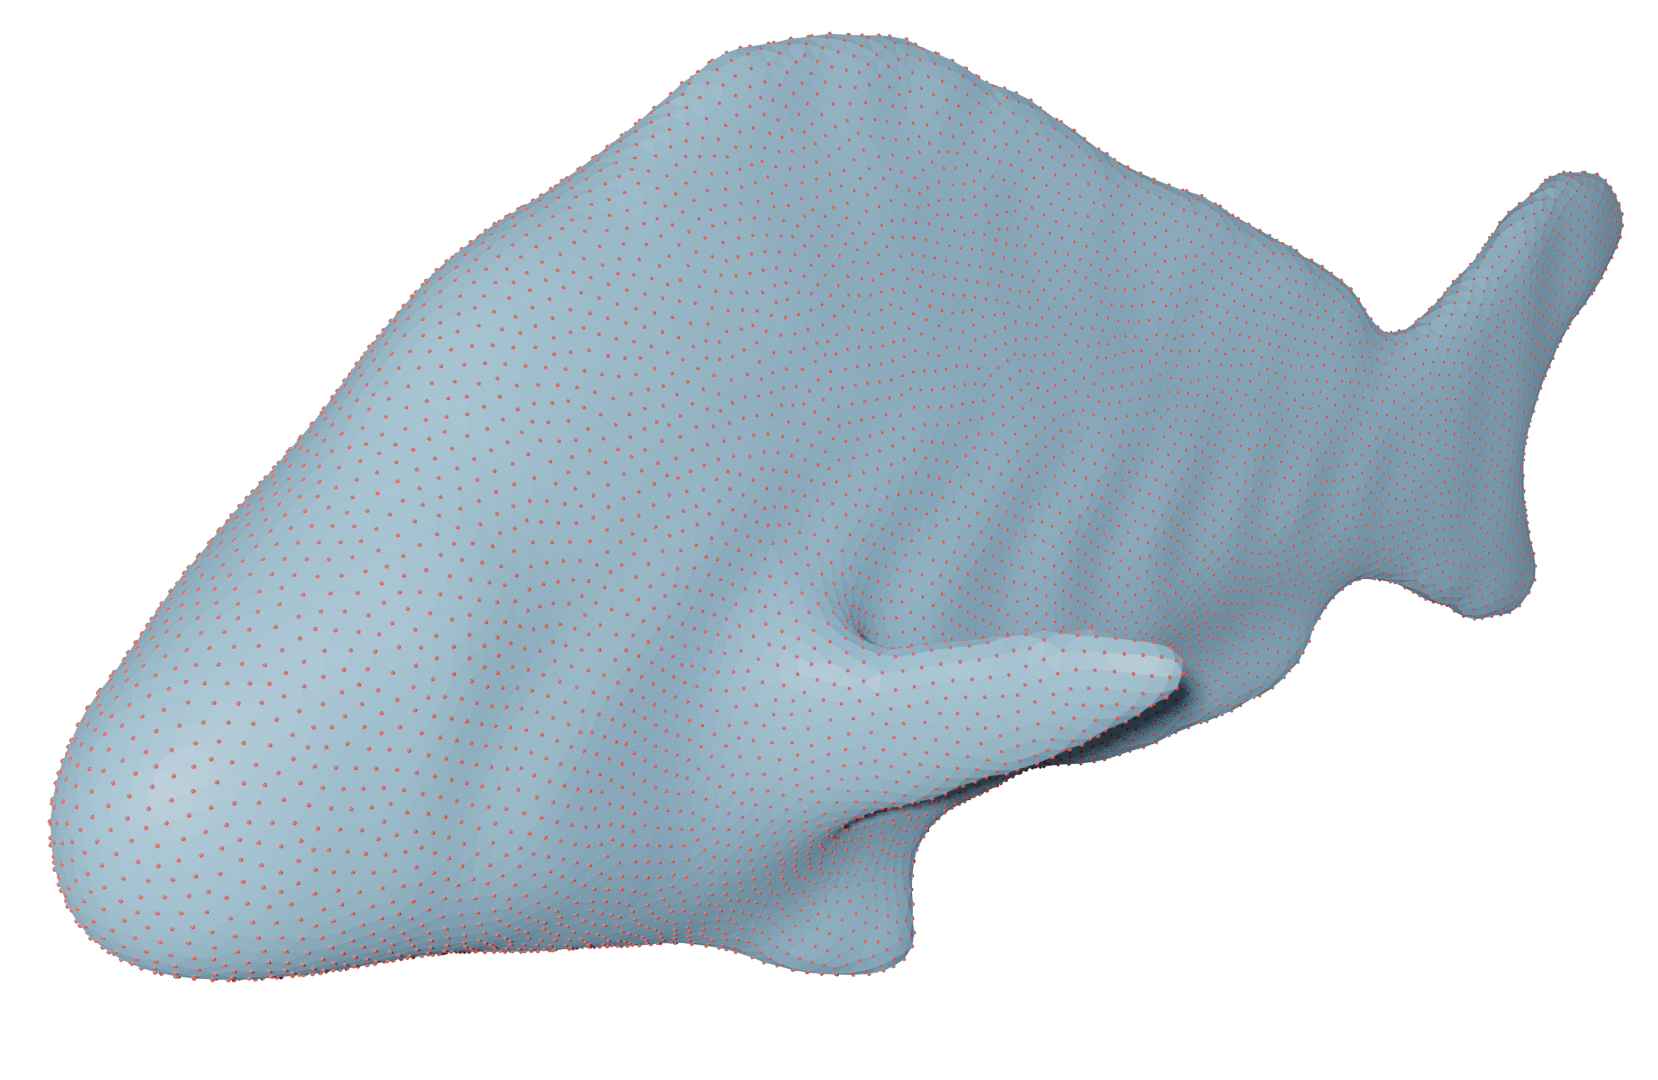
\includegraphics[width=.23\linewidth]{curve_meshing_in_shell_tex/figs/fish/fish002}
    \hfill
    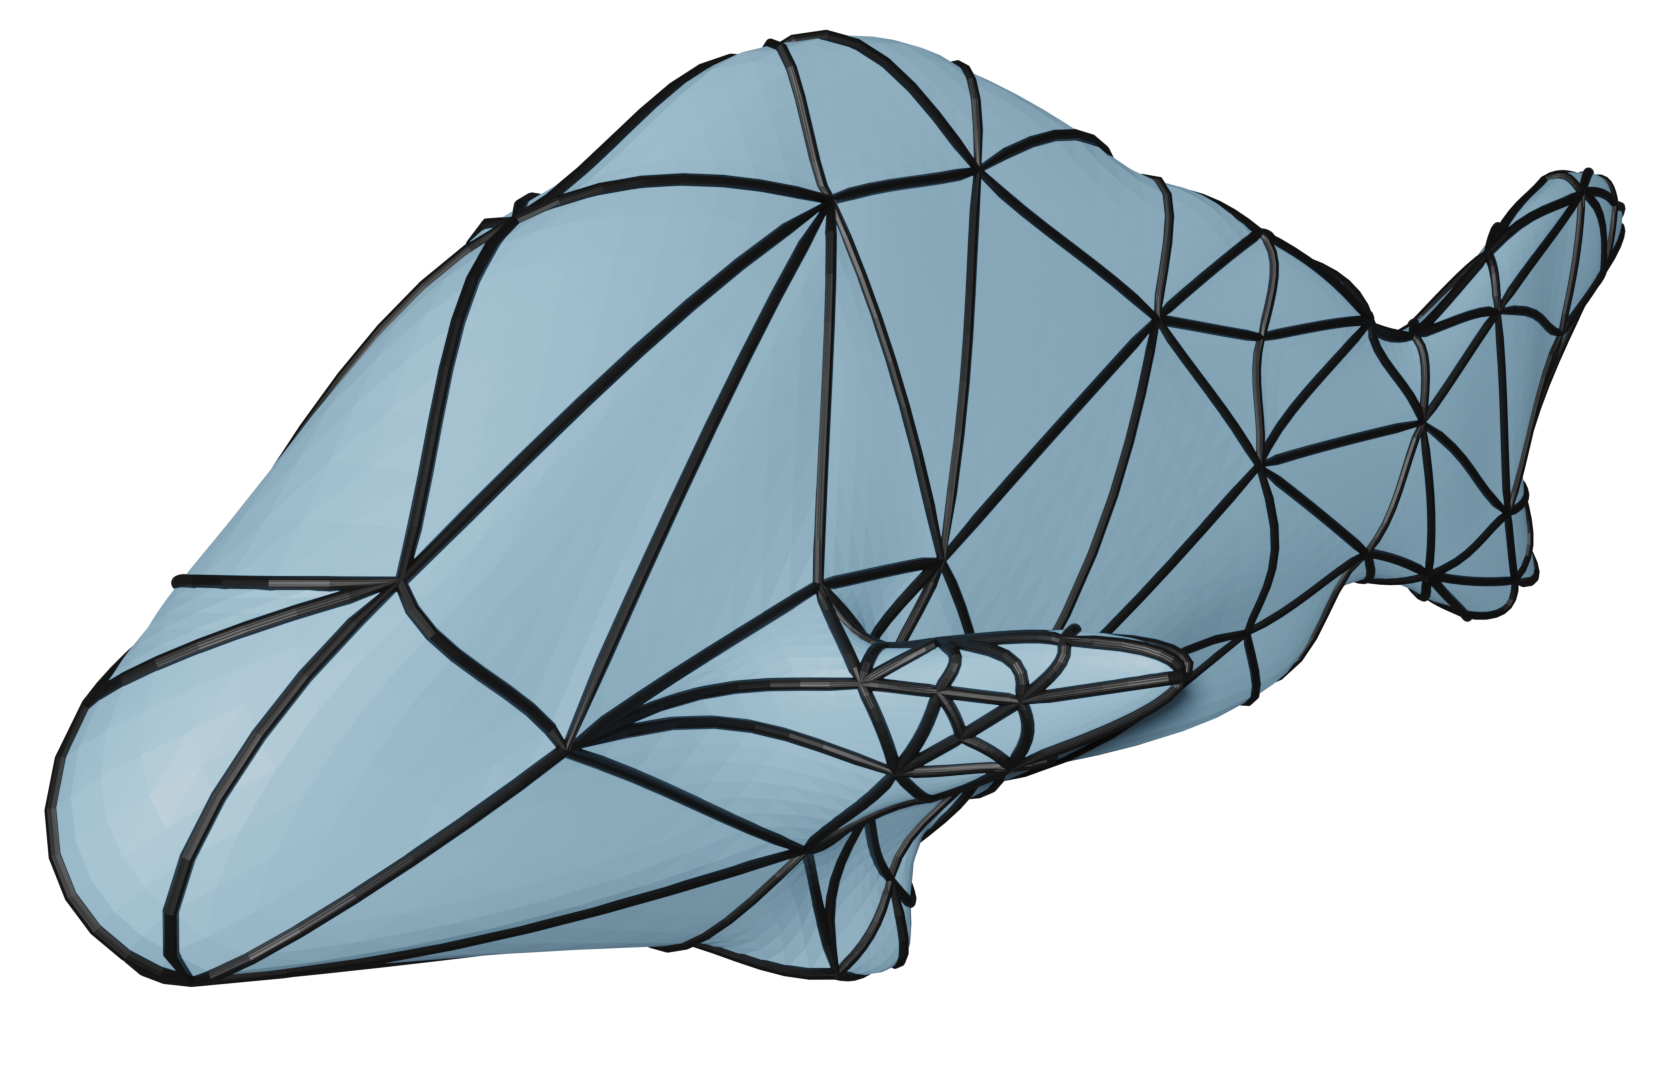
\includegraphics[width=.23\linewidth]{curve_meshing_in_shell_tex/figs/fish/0003}\hfill
    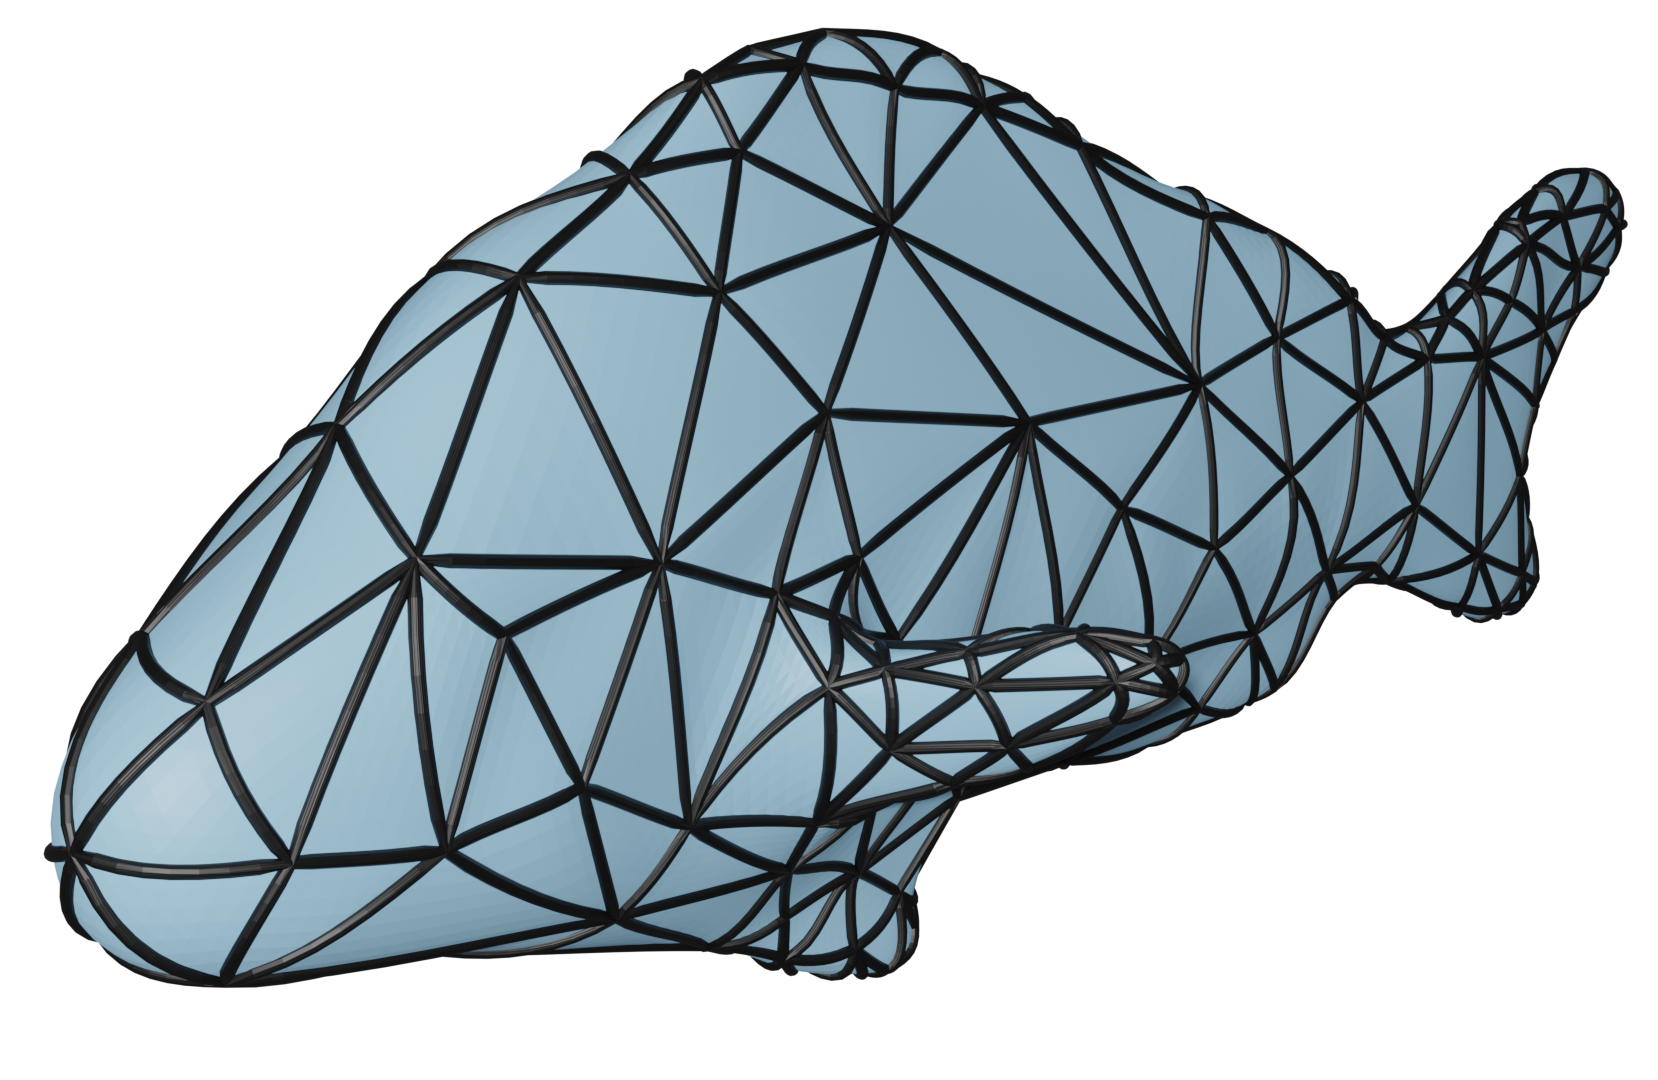
\includegraphics[width=.23\linewidth]{curve_meshing_in_shell_tex/figs/fish/0001}\hfill
    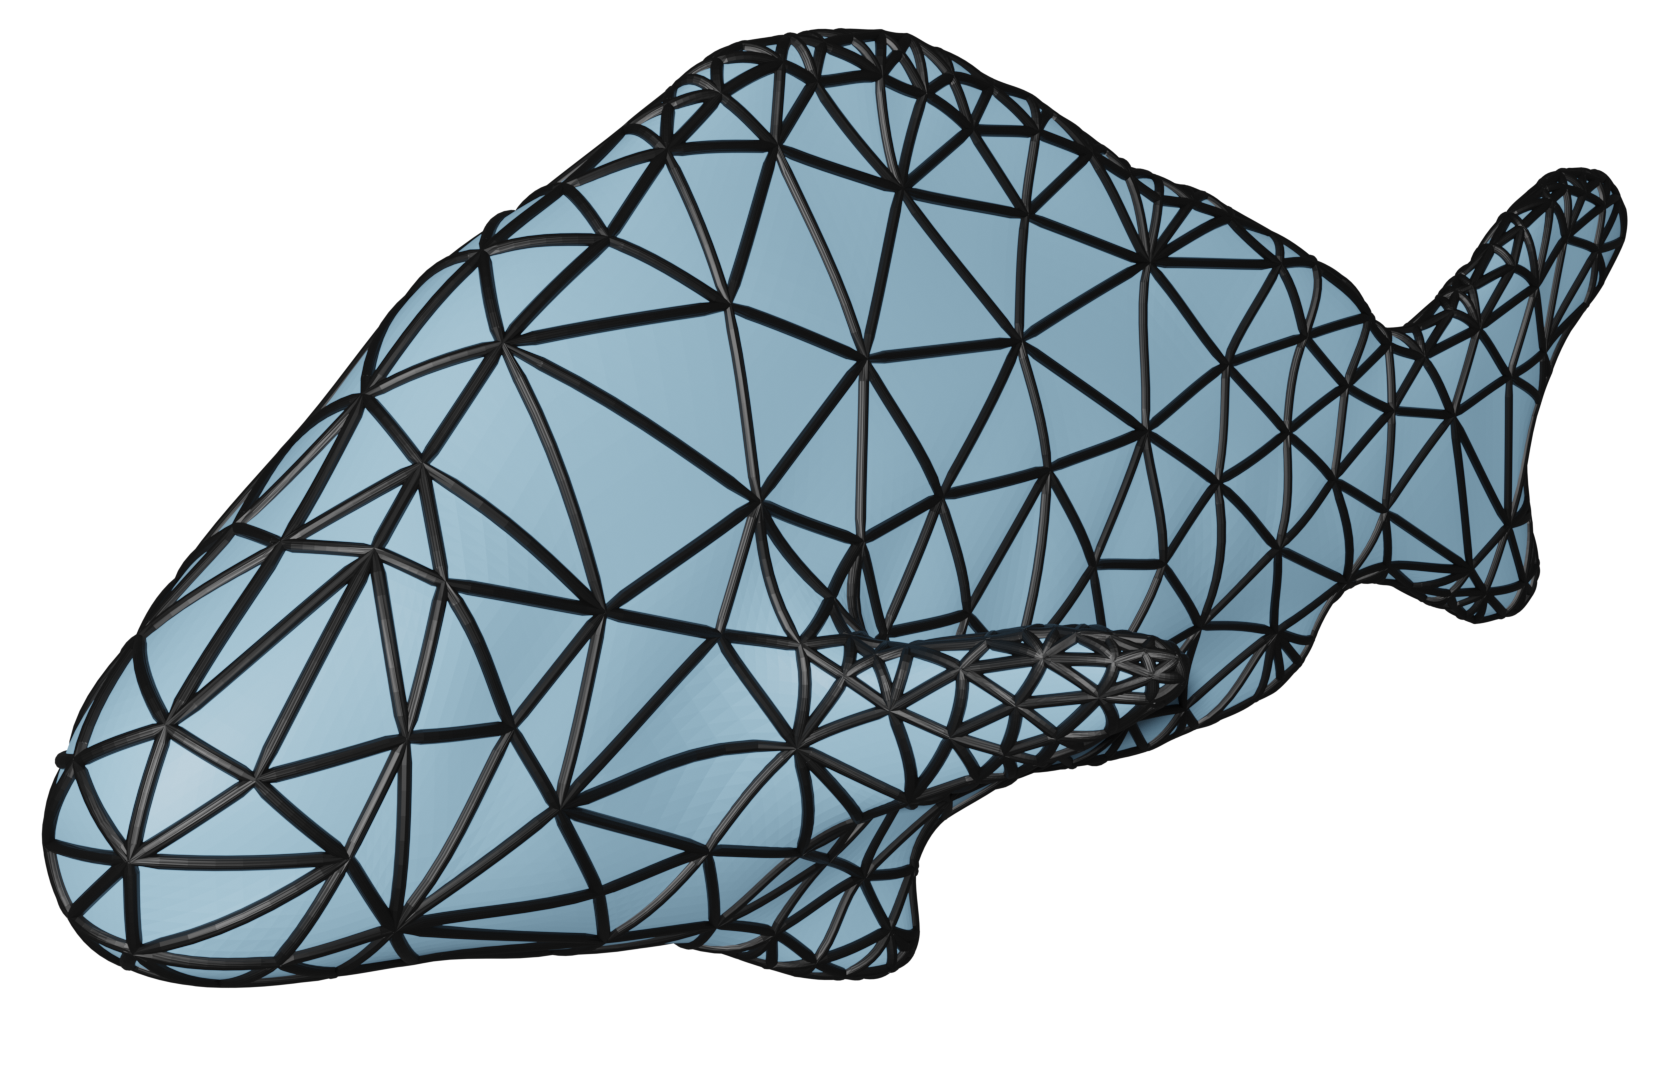
\includegraphics[width=.23\linewidth]{curve_meshing_in_shell_tex/figs/fish/0004}\par
    \parbox{.23\linewidth}{\centering Input}\hfill
    \parbox{.23\linewidth}{\centering $\varepsilon =5\times 10^{-3}$}\hfill
    \parbox{.23\linewidth}{\centering $\varepsilon =  10^{-3}$}\hfill
    \parbox{.23\linewidth}{\centering $\varepsilon = 5\times 10^{-4}$}
    \caption{A model simplified with different distances.}
    \label{bichon:fig:distance}
\end{figure}

\subsection{Distance Bound}\label{cumin:sec:distance}

In the previous section, we explained how to generate a curved shell $\prS$ that satisfies~\ref{def:curved-mesh}. To ensure that the middle surface of $\prS$ has a controlled distance from the points in $\P$, we interleave a distance check in the construction of $\widetilde\omega^k$ after each local operation. Formally, after every local operation we use the mapping $\phi^k$ to map every point $p_i\in\P$ to $\widetilde p_i = \phi^k(p_i)$ a point on the coarse curved middle surface of $\prS$ and, if $\|p_i-\widetilde p_i\| \geq \varepsilon$ we reject the operation. The initial shell is trivially a valid initialization as $\phi^k$ is identity and thus, the distance is zero. Note that, $\widetilde p_i$ is not necessarily the closest point to $p_i$ on $\partial\T$, thus $\|p_i-\widetilde p_i\|$ is an upper bound on the actual pointwise distance. Figure~\ref{bichon:fig:distance} shows the effect of the distance bound on the surface; a small distance will lead to a denser mesh with more details, while a {large} one will allow for more coarsening.



%%%%%%%%%%%%%%%%%%%%%%%%%%%%%%%%%%%%%%%%%%%%%%%%%%%%%%%%%%%%%%%%
%%%%%%%%%%%%%%%%%%%%%%%%%%%%%%%%%%%%%%%%%%%%%%%%%%%%%%%%%%%%%%%%
\subsection{Tetrahedral Meshing}\label{cumin:sec:tets}

The outcome of the previous stage is a curved tetrahedralization of $\prS$ that closely approximates $\M$ with linear (``flat'') boundaries. We now consider the problem of filling its interior (and optionally its exterior) with a tetrahedral mesh, a problem known as  \emph{conforming boundary preserving} tetrahedralization. 

%After the linear tetrahedralization, we have a valid (according to Definition~\ref{def:curved-mesh}) output which we further improve by performing local operations on the curved mesh.

\begin{figure}
    \centering
    % \includegraphics[width=.39\linewidth]{curve_meshing_in_shell_tex/figs/tet12}\hfill
    % \includegraphics[width=.39\linewidth]{curve_meshing_in_shell_tex/figs/tet34}\hfill
    % \includegraphics[width=.19\linewidth]{curve_meshing_in_shell_tex/figs/tet5}
    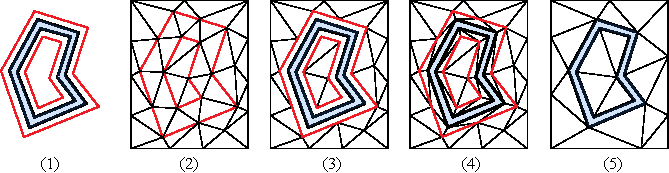
\includegraphics[width=\linewidth]{curve_meshing_in_shell_tex/figs/illustrations/conforming-overview.pdf}
    \caption{Two dimensional overview of the five steps of our boundary preserving tetrahedral meshing algorithm.}
    \label{bichon:fig:conforming-overview}
\end{figure}

Several solution exists for this problem (Section~\ref{cumin:sec:rel:linear}) and the most common implementation is TetGen~\cite{tetgen}. Most algorithms refine the boundary, which allows {deriving} bounds on the quality of the tetrahedral mesh. However, in our setting, this is problematic, as any change will have to be propagated to the curved shell. To avoid coupling the volumetric meshing problem with the curved shell coarsening, while technically possible it is very challenging to implement robustly, we opt for using a tetrahedral meshing algorithm that preserves the boundary exactly. Not many algorithms support this additional constraint, the only one with a public implementation is the widely used TetGen algorithm. However, we discovered that, when this option is used, it suffers from robustness issues.
%
To solve this problem in our specific setting, we propose in the following five step algorithm (Figure~\ref{bichon:fig:conforming-overview}) taking advantage of the availability of a shell, based on the  TetWild~\cite{hu2018tetrahedral} algorithm.

\paragraph{Step 1.}
To generate a boundary preserving linear mesh, we first exploit the shell to extrude the bottom surface $B$ (and top $T$) {further} by a positive (potentially small) constant $\delta$ such that the newly extruded bottom surface $B_e$ (and top $T_e$) does not self-intersect. The space between $B$ and $B_e$ (and between $T$ and $T_e$) consists of prisms {divided} into positive tetrahedra. 

\paragraph{Step 2.}
Then we insert $B_e$ and $T_e$ in a background mesh $\B$ generated following TetWild algorithm (\cite[Section 3.1]{hu2018tetrahedral}), that is, we use the triangle of $B_e$ and $T_e$ as the input triangle meshes for the first stage of the TetWild algorithm, which inserts them into a background mesh $\B$, so that
each input triangle is a union of faces of refinement of $\B$.


We interrupt the algorithm after the  binary space partitioning (BSP) subdivision (and before the TetWild mesh optimization \cite[Section 3.2]{hu2018tetrahedral})
to obtain a positive tetrahedral mesh in rational coordinates with a surface with the same geometry of $B_e$ and $T_e$, but possibly different connectivity as TetWild might refine it during the BSP stage.

\paragraph{Step 3.}
Our original goal was to compute a mesh conforming to $B$ and $T$, but we could not do it directly with TetWild as they might be refined. We now replace the mesh generated by TetWild between $B_e$ and $T_e$ with another one conforming to $B$ and $T$. To achieve this, we delete all tetrahedra between $B_e$ and $T_e$, and insert the surfaces $B$ and $T$, which will ``float'' in the empty space between $B_e$ and $T_e$. We now want to fill the space between $B$ and $B_e$ with positive tetrahedra conforming to the surfaces $B$ and $T$. 

\paragraph{Step 4.}
Every prism $P$, made by a bottom triangle $B^T$ and a bottom extruded triangle $B_e^T$ and its corresponding bottom extruded refined triangle $B_e'^T \in \B$, can be tetrahedralized without refining $B$: That is, we first decompose the prism $B^T, B_e^T$ in tetrahedra (always possible by construction), then refine every tetrahedron touching $B_e'^T$. By repeating the same operation on the space between $T$ and $T_e$ we will have a positive linear boundary conforming tetrahedral mesh of $B$ and $T$. 

\paragraph{Step 5.}
The tetrahedra generated in the previous step will have rational coordinates and will also likely have low quality. To round the coordinates to floating-point representation and to improve their quality, we use the mesh optimization stage of TetWild, with the minor variant of keeping the vertices and edges on $B$ and $T$ frozen. Note that the vertices in $B$ and $T$ are already roundable to floating-point representation, as they were part of the input.


\begin{figure}
    \centering
    \parbox{0.02\linewidth}{~}\hfill\hfill
    \parbox{.47\linewidth}{\centering Mean}\hfill
    \parbox{.47\linewidth}{\centering Max}\par
    %%%%%
    \parbox{0.02\linewidth}{\centering\rotatebox{90}{\scriptsize{Model Count}}}\hfill\hfill
    \parbox{.47\linewidth}{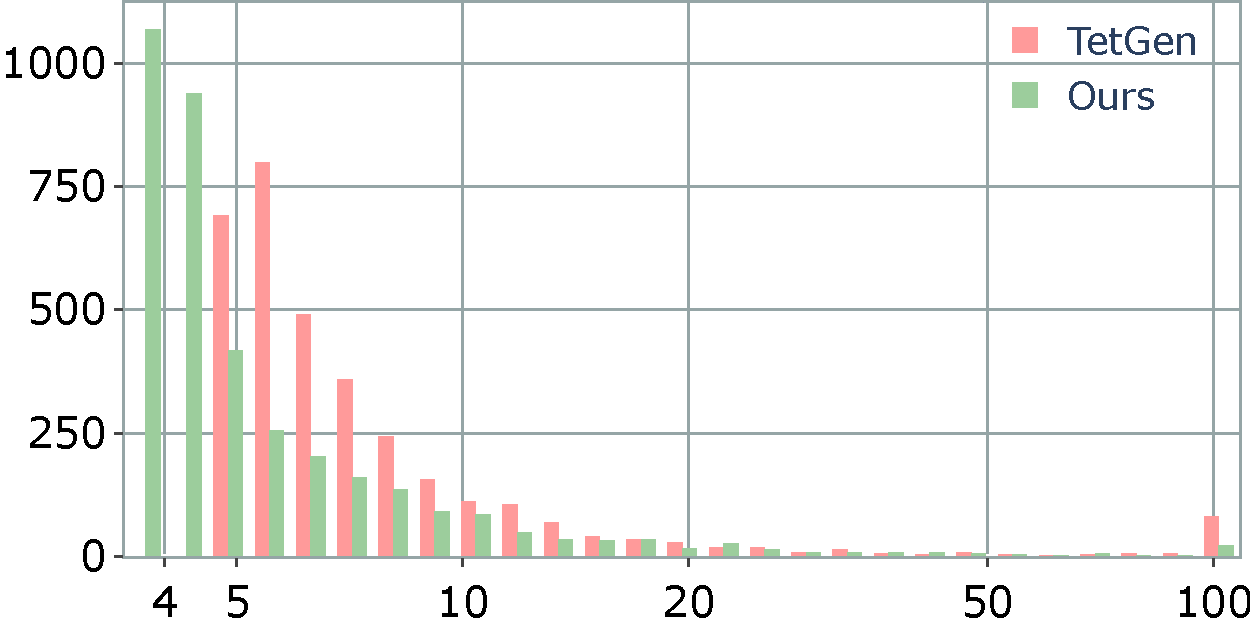
\includegraphics[width=\linewidth]{curve_meshing_in_shell_tex/figs/stats/tetgen_meanE}}\hfill
    \parbox{.47\linewidth}{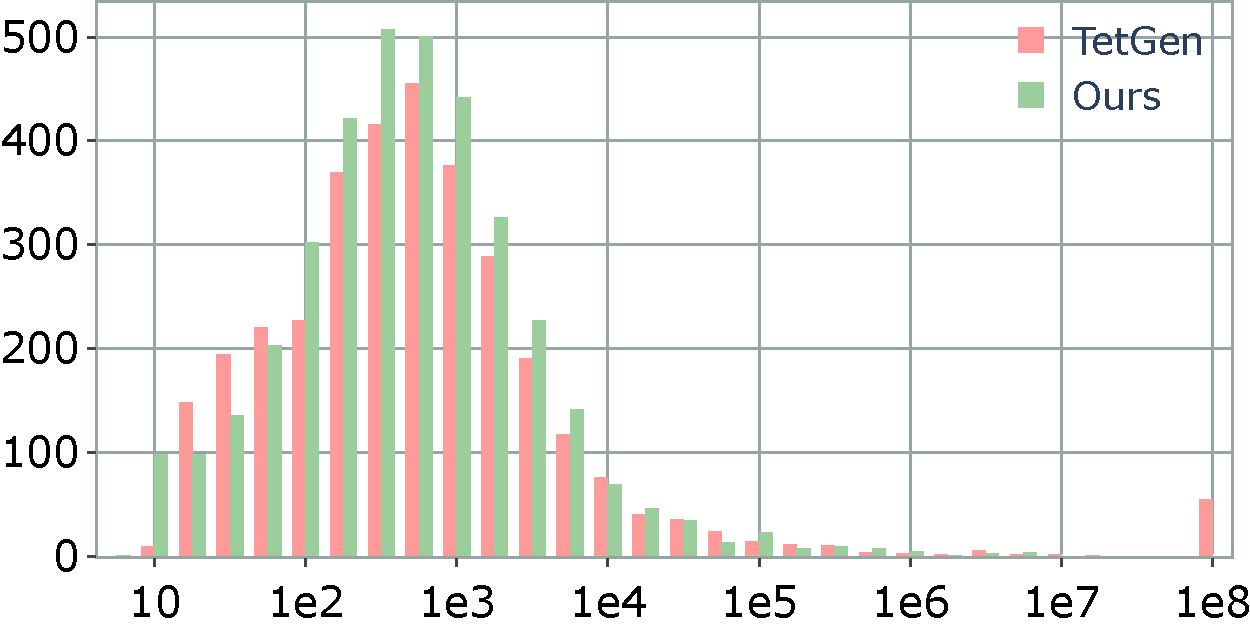
\includegraphics[width=\linewidth]{curve_meshing_in_shell_tex/figs/stats/tetgen_maxE}}\par
     \scriptsize{AMIPS Energy}
    \caption{Histogram of mean and maximum conformal AMIPS energy~\cite{rabinovich2017scalable} of the output of our method and TetGen.}
    \label{bichon:fig:energy-max-avg}
\end{figure}

\begin{figure}
    \centering
    \parbox{.7\linewidth}{\centering
    \parbox{0.02\linewidth}{\centering\rotatebox{90}{\scriptsize{Model Count}}}\hfill
    \parbox{.95\linewidth}{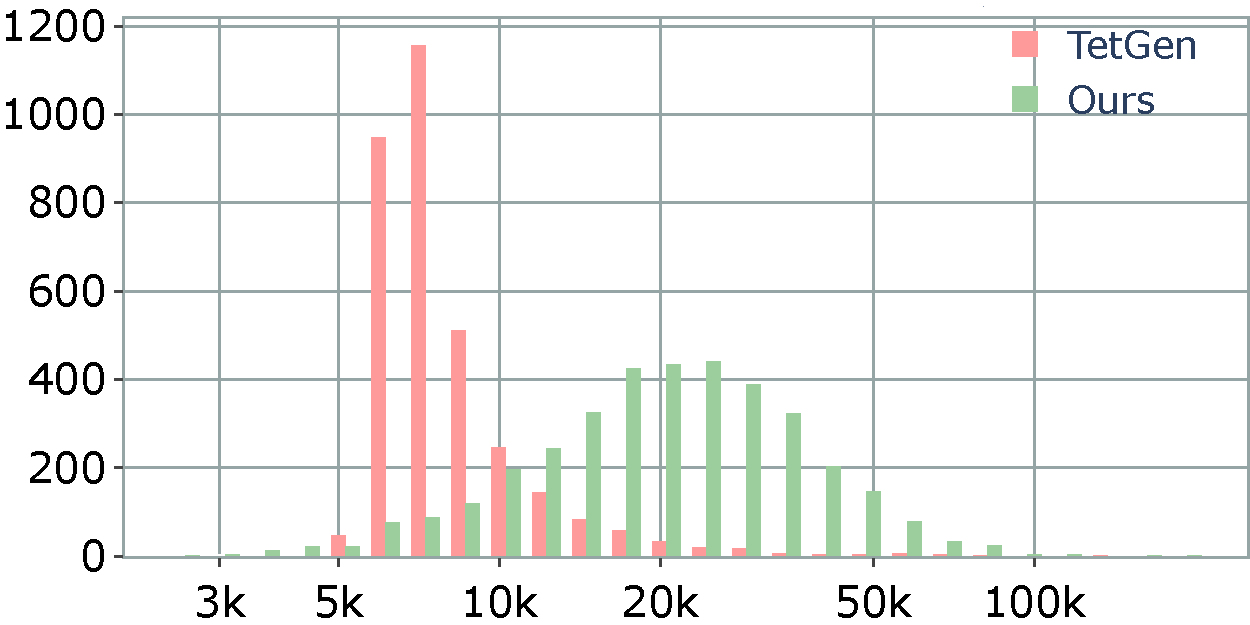
\includegraphics[width=\linewidth]{curve_meshing_in_shell_tex/figs/stats/tetgen_TO}}\par
    \scriptsize{Tetrahedra Number}
    }
    \caption{Histogram of output tetrahedra number for TetGen and {our} method. }
    \label{bichon:fig:numt}
\end{figure}

\paragraph{Boundary preserving TetGen comparison}
We compared our conforming tetrahedral meshing algorithm (Section~\ref{cumin:sec:tets}) with TetGen on the linear shells (triangle meshes) of 3522 models from the Thingi10k dataset, giving each model sufficient computing resources (2 hours maximum running time and 32GB memory usage). Inheriting the robustness from TetWild, our method successfully processed all the inputs while preserving the triangulation, while TetGen fails on 224 models (215 models are not conforming, and 9 models have no output).  In Figure~\ref{bichon:fig:energy-max-avg}, we show the average and maximum element quality of the output of our method and TetGen. Our method has {a} better average and maximum output quality than TetGen. Note that in the quality plot, the ``tail'' of TetGen's distribution is longer than ours. The maximum average energy of TetGen's output and ours are $3\times 10^8$ and $3 \times 10^5$ respectively. The largest maximum energy of TetGen's output and ours are $3\times 10^{12}$ and $7 \times 10^6$ respectively. Our method generates denser output (Figure~\ref{bichon:fig:numt}), but our focus is on robustness instead of efficiency in this step.



\paragraph{Curved Tetrahedral Mesh Optimization}
After generating the conforming linear tetrahedral mesh. we stitch it with the tetrahedralized $\prS$ to obtain a valid output mesh $\T^k$ {(Definition~\ref{def:curved-mesh}).} However, its quality might be low, in particular in the curved region, as $\prS$ can be thin with large triangles. To improve the quality of  $\T^k$ we adapt the local operation of a linear pipeline to our curved settings. We propose three local operations: smoothing, collapse, and flip. 
Since the surface of $\T^k$ is already coarse {and} of high quality, {as} part of the definition of $\phi^k$, we prevent any local operation from changing it. We validate every local operation (i.e., check the positivity of $\T^k$) using the convex-hull property~\cite{johnen2013geometrical} and reject the operation if it is violated.
Our local operations are prototypical, and we leave as future work a more comprehensive study of curved mesh optimization.
 
\paragraph{Smoothing.} As for the linear case, we compute the total energy of a vertex $v$ by summing up the energies of the tetrahedra adjacent to it, which we compute on 56 regularly sampled points. 
We then perform gradient descent {for} all high-order nodes in the one-ring neighborhood of $v$. That is, we collect all edge nodes, face nodes, and cell nodes of the one-ring neighborhood of $v$. Differently {from} the linear case, the optimization is expensive since the nodes neighborhood typically contains hundreds of nodes.

\paragraph{Collapse and Swap}
The collapse and swap are the same as in a linear mesh, and we place the high-order nodes of the newly created face on the linear flat face.

\section{Local Operations for High Order Meshing}
\label{app:local-ops}
Figure~\ref{prism:fig:local_operations} introduce a set of \emph{valid} local operations to modify the shell, including edge split, edge collapse, edge flip and vertex smoothing. 
The operations are an analogue of the triangle mesh edit operations \cite{dunyach2013adaptive}, 
by simultaneously editing the shared connectivity of bottom, middle and top surface of the shell.
Chapter~\ref{chp:shell} Theorem 3.7 outlines invariant conditions, which maintains the shell projection to be bijective. 

Our algorithm adopts and extends the local operations therein to the high order setting. In addition to the existing conditions, we also validate the curved volumetric mesh in the shell.
The algorithm maintains the global intersection free bottom (top) surface with a dynamic hash grid \cite{teschner2003optimized}. Then for each prism, we check the positivity (defined by the determinant of Jacobian of the geometric map) of the prismatic element (each decomposed into three tetrahedra).

In the presence of feature annotation and feature straightening (Section \ref{cumin:sec:features-pres}) more care is taken to maintain the valid correspondence between the grouped feature chains and the curved edges: 
edge flip is disabled on the edges annotated as features; collapse is only allowed when it does not degenerate the chain, and the two endpoints of the edge is on the same chain. 
Since we require a map from the original input edges, we insert additional degree of freedoms in the input mesh. When performing edge split, the insertion of the new vertex is queried among the pre-image of the current edge, as an existing vertex of the input. For vertex smoothing (more specifically pan), the target location is limited to the set of input vertices.

\section{Feature Preserving Curved Shell}\label{cumin:sec:features-pres}


\begin{figure}
    \centering
    % 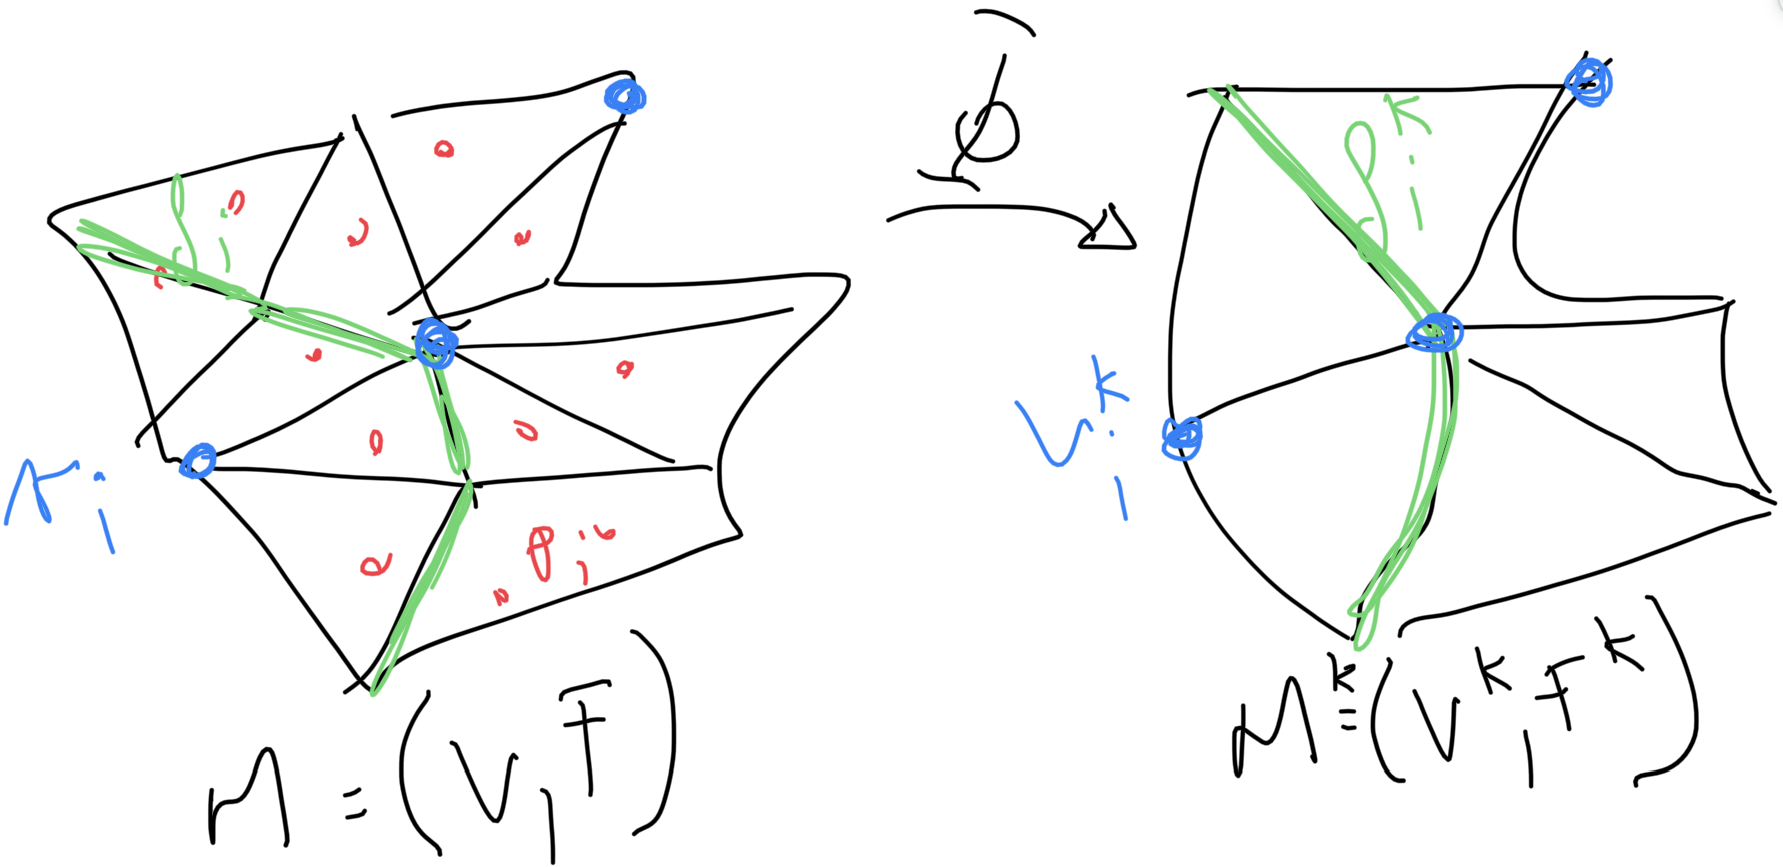
\includegraphics[width=.7\linewidth]{curve_meshing_in_shell_tex/figs/input-output}
    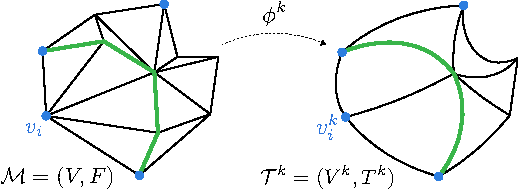
\includegraphics[width=.75\linewidth]{curve_meshing_in_shell_tex/figs/illustrations/input-output-feature.pdf}
    \caption{Input triangle mesh with features and output curved mesh with feature preserved equipped with bijective map $\phi^k$.}
    \label{bichon:fig:input-output-feature}
\end{figure}

% We are now ready to extend the previous construction to features. 
\paragraph{Input}
We enhance the input to additionally include a set of feature edges $f_i\in\F$ and feature vertices $v_i\in\V$ such that no triangle in $F$ has more than one feature edge (Figure~\ref{bichon:fig:input-output-feature} left). (This property can be satisfied on any generic mesh by performing 1-to-3 refinement on every triangle with more than one feature edge). 

\paragraph{Output}
Since the input has features, the output curved mesh $\T^k$ will also have curved {feature} edges $f_i^k\in\T^k$, feature vertices $v_i^k\in\V^k$, and the bijective map $\phi^k$ preserves features by bijectively mapping $\F$ to $\F^k$ and $\V$ to $\V^k$. Our {method} makes no assumption on the topology and ``quality'' of the features. If the features are reasonable, it will produce {a} high-quality mesh, while if the features are close our algorithm will preserve them and result in smaller triangles on the surface. (Figure~\ref{bichon:fig:bad-features}).

\begin{figure}
    \centering
    % \includegraphics{}
    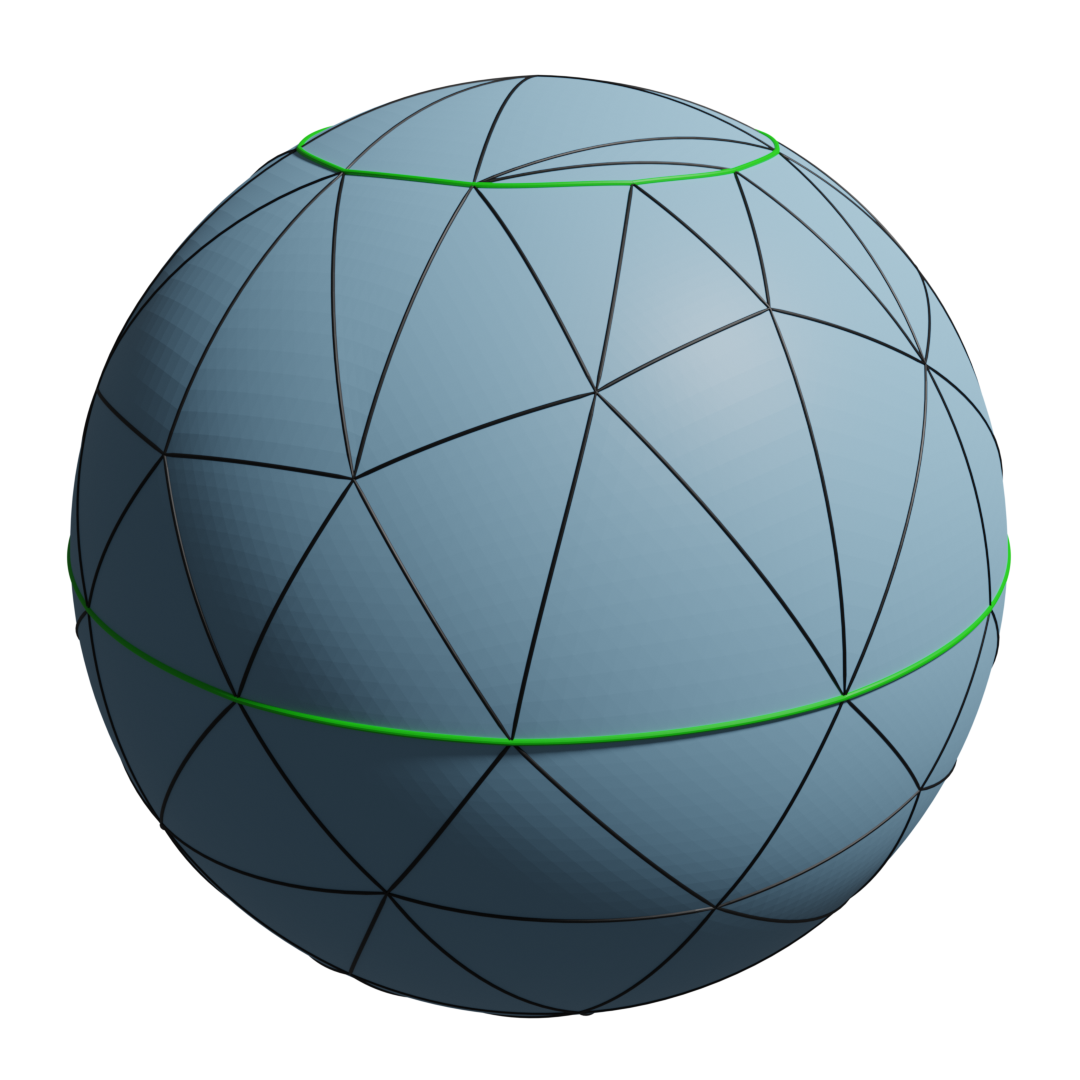
\includegraphics[width=.24\linewidth]{curve_meshing_in_shell_tex/figs/sphere/0001}\hfill
    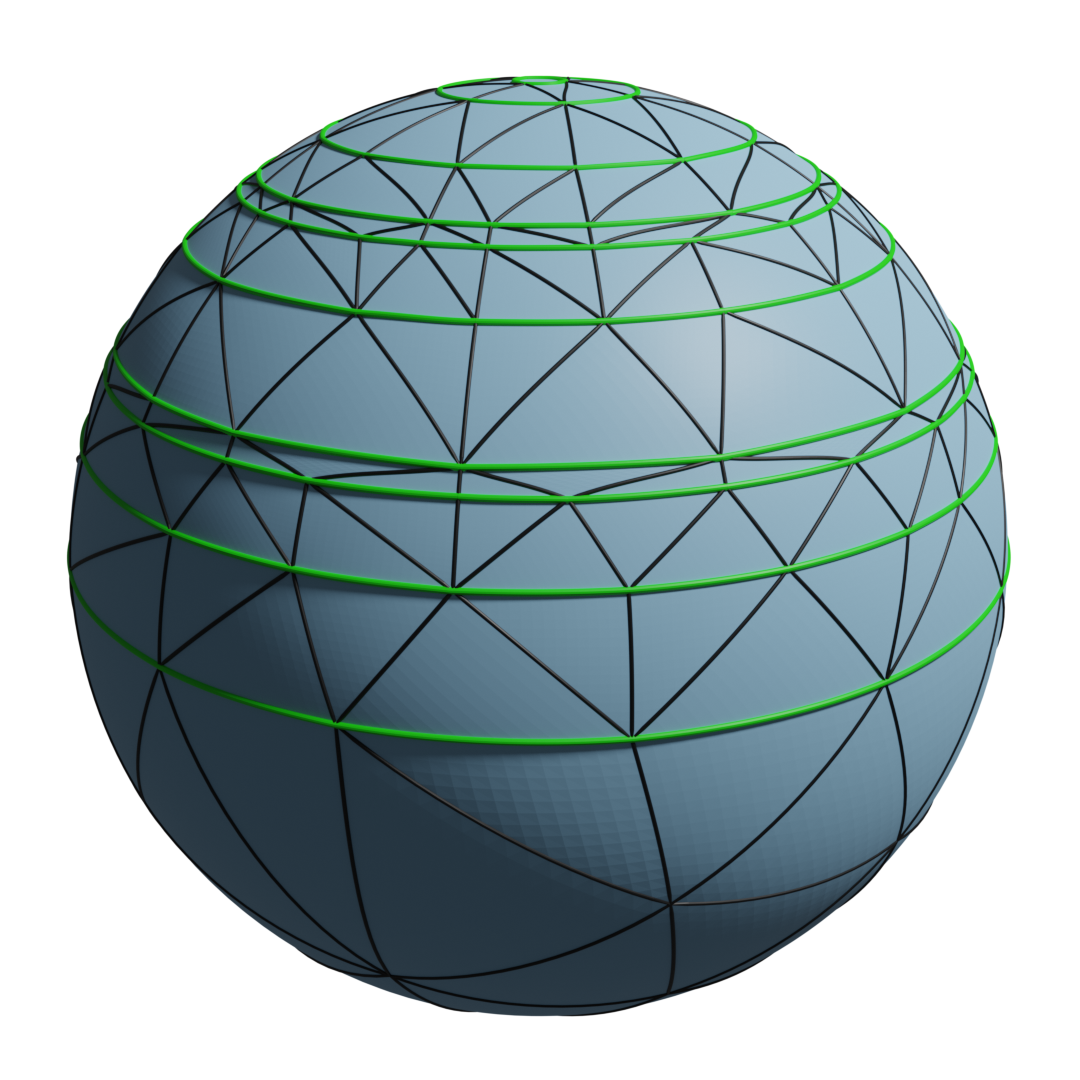
\includegraphics[width=.24\linewidth]{curve_meshing_in_shell_tex/figs/sphere/0002}\hfill
    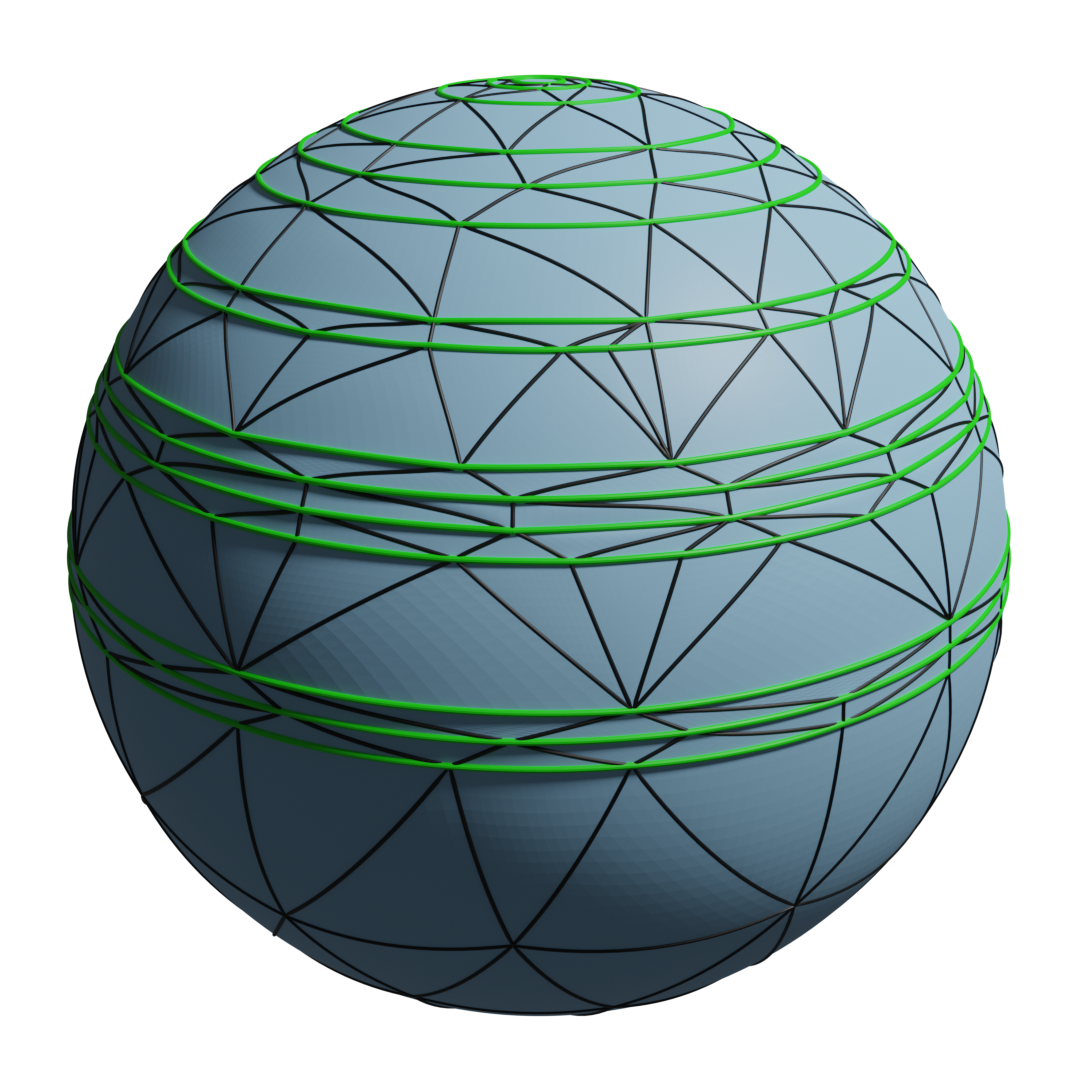
\includegraphics[width=.24\linewidth]{curve_meshing_in_shell_tex/figs/sphere/0003}\hfill
    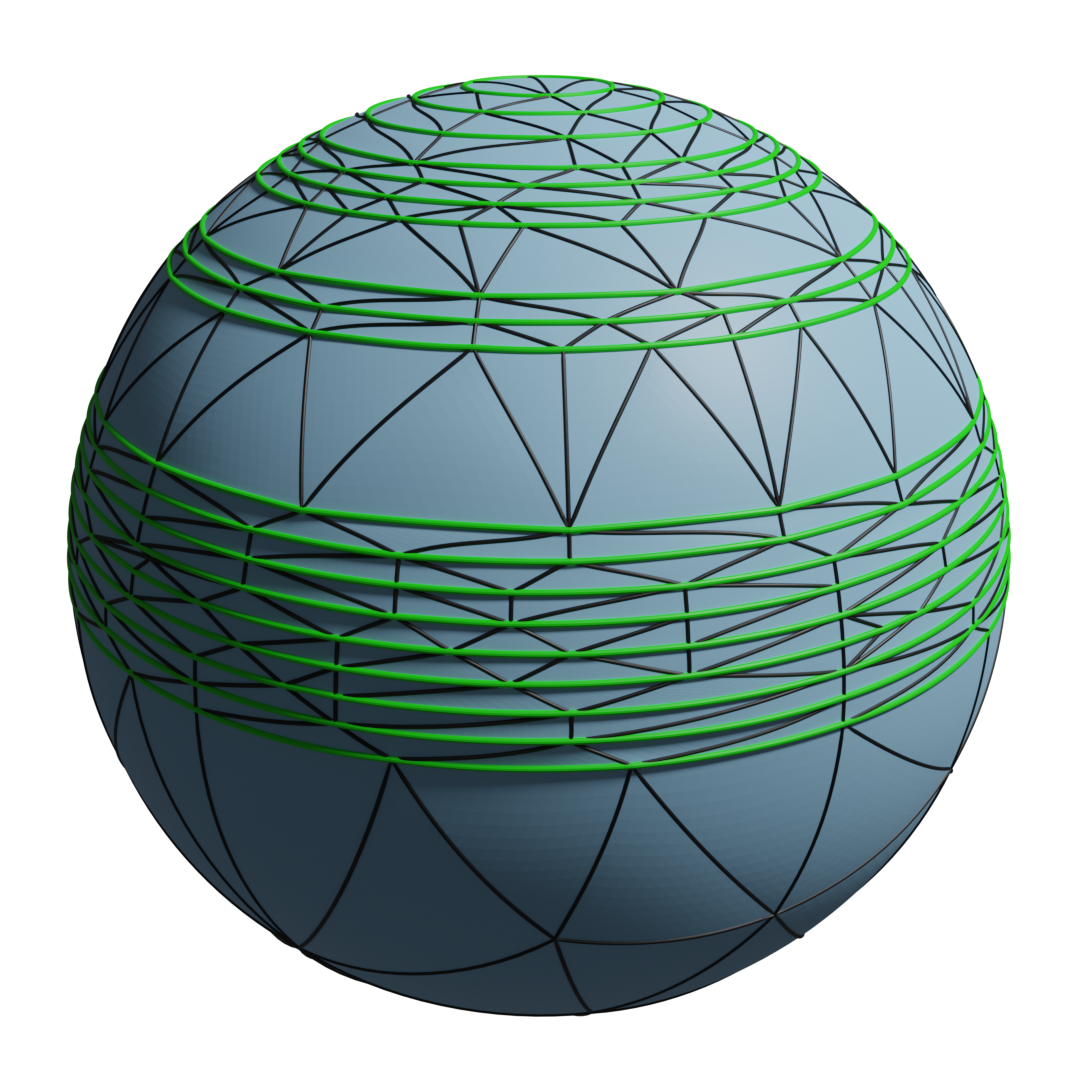
\includegraphics[width=.24\linewidth]{curve_meshing_in_shell_tex/figs/sphere/0004}
    \caption{A sphere with different marked features (green). As we increase the number of features our algorithm will preserve them all but the quality of the surface suffers.}
    \label{bichon:fig:bad-features}
\end{figure}


\begin{figure}
    \centering
    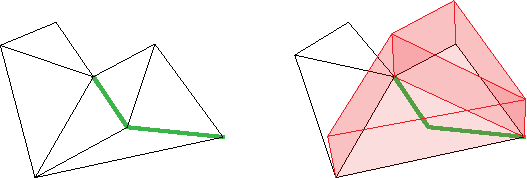
\includegraphics[width=.7\linewidth]{curve_meshing_in_shell_tex/figs/illustrations/not-feat-pres.pdf}
    \caption{Input feature (green) is not preserved after traditional shell simplification.}
    \label{bichon:fig:not-feat-pres}
\end{figure}

The previous construction generates valid curved tetrahedral meshes and the bijective map $\phi^k$ based on the construction of~\cite{jiang2020bijective}. However, the shell construction cannot coarsen features{:} the authors suggest {freezing} them. For instance, when performing an edge collapse on the feature, the new coarse edge (orange) will not map to the feature (green) anymore (Figure~\ref{bichon:fig:not-feat-pres}). 
To ensure feature preservation we extend Definition~\ref{def:curved-mesh}.
\begin{definition}\label{def:curved-features}
We call a curved mesh $\T^K$ and its mapping $\phi^k$ from $\M$ \emph{valid and feature preserving} if they are valid (Definition~\ref{def:curved-mesh}) and $\phi^k$ bijectively maps $\F$ to $\F^k$ and $\V$ to $\V^k$
\end{definition}
As for the non-feature preserving case, we always aim to maintain a valid feature preserving $\T^k$.


\begin{figure}
    \centering
    % \includegraphics[width=\linewidth]{curve_meshing_in_shell_tex/figs/pipeline}
    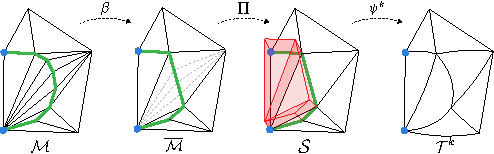
\includegraphics[width=\linewidth]{curve_meshing_in_shell_tex/figs/illustrations/stage-1.pdf}
    \caption{Overview of the construction of the first stage of our pipeline.}
    \label{bichon:fig:stage-1}
\end{figure}

\begin{figure}
    \centering
    % \includegraphics[width=\linewidth]{curve_meshing_in_shell_tex/figs/pipeline}
    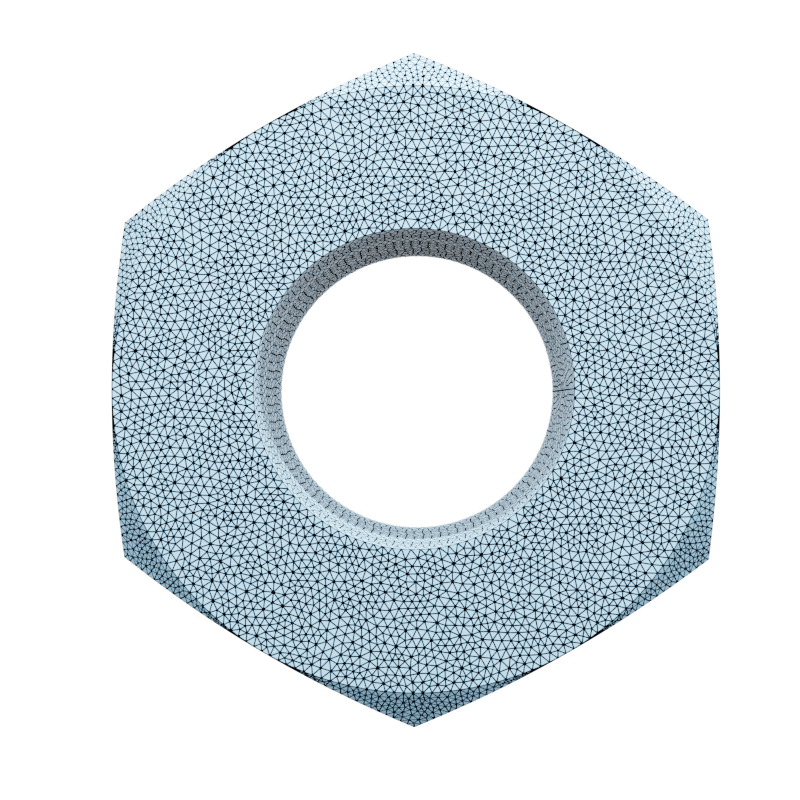
\includegraphics[width=0.33\linewidth]{curve_meshing_in_shell_tex/figs/snap_abc6/0001.png}\hfill
     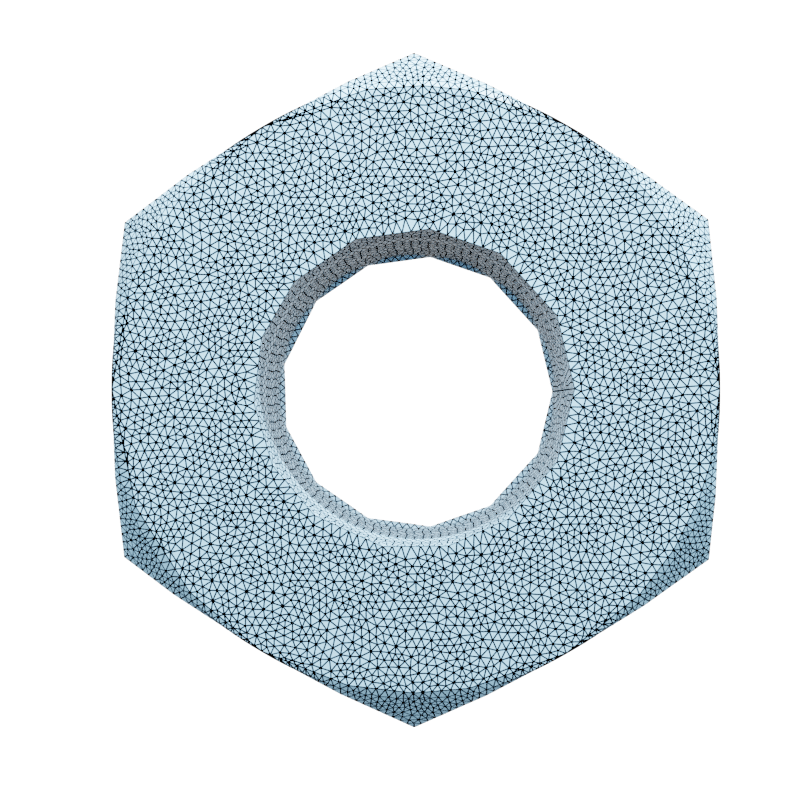
\includegraphics[width=0.33\linewidth]{curve_meshing_in_shell_tex/figs/snap_abc6/0002.png}\hfill
     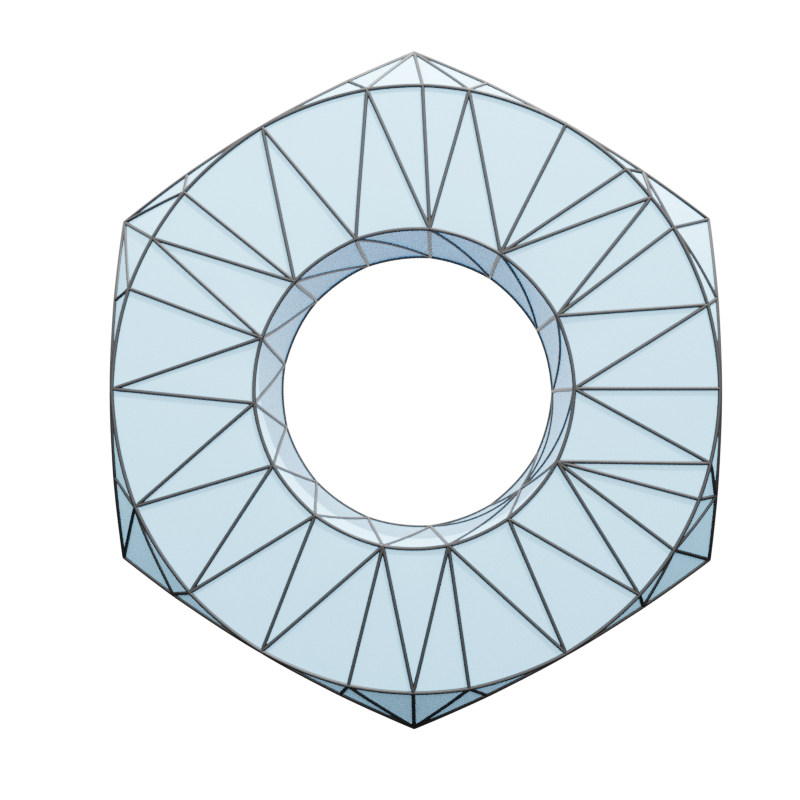
\includegraphics[width=0.33\linewidth]{curve_meshing_in_shell_tex/figs/snap_abc6/0003.png}\par
     \parbox{.33\linewidth}{\centering Input mesh}\hfill
     \parbox{.33\linewidth}{\centering Snapped mesh}\hfill
     \parbox{.33\linewidth}{\centering Curved mesh}
    \caption{The input mesh has feature edges snapped, to create a valid shell, as well as the curved mesh.}
    \label{bichon:fig:ex-snapping}
\end{figure}

To account for features, we propose to change the prismatic map $\Pi$, that is, we only need to change the first stage. This is done by snapping the input features  (Section~\ref{cumin:sec:snapping}). That is, we modify $\M$ to ``straighten'' the feature to ensure that the coarse prismatic projection preserves them and construct a mapping $\beta$ between the {straight} mesh $\overline\M$ and $\M$ (Figure~\ref{bichon:fig:ex-snapping}). 

The outcome {is} a \emph{valid} shell $\PS$ with respect to the {straight} surface $\overline\M$ (i.e., $\overline\M$ is a section $\PS$) that preserve features, the prismatic projection $\Pi$, and the bijective map $\beta$ that can be directly used in the curved pipeline (Section~\ref{cumin:sec:curved-pipeline}). That is, the mapping  $\phi^k$ will be defined as $\phi^k = \beta \circ \Pi \circ \psi^k$.

As for the non-preserving feature pipeline we ensure that our conditions are always met, starting {from} a trivial input and rejecting operations violating them. Our goal is to modify the input mesh $\M$ and create $\overline\M$ by moving its vertices. In such a way, the mapping $\beta$ is simply barycentric. To guarantee bijectivity of $\phi^k$ we need to ensure that all {mappings} composing it are bijective, in particular $\beta$. To ensure that $\beta$ is bijective it is enough that $\overline\M$ is self-intersection free (guaranteed by the shell construction) and that all its triangles have positive area. By straightening the features of $\M$ we ensure that the edges of the prism will map to the feature. Thus, $\phi^k$ will be feature preserving.


\begin{figure}
    \centering
    % \includegraphics[width=0.5\linewidth]{curve_meshing_in_shell_tex/figs/feat-gr}
    \includegraphics[width=0.65\linewidth]{curve_meshing_in_shell_tex/figs/illustrations/feat-gr.pdf}
    \caption{The input edges feature (green) are grouped together in poly-lines and categorized in graph (left) and loops (right). For every graph we add the nodes (blue) to the set of feature vertices.}
    \label{bichon:fig:feat-gr}
\end{figure}

\paragraph{Feature Grouping.}
The first step of our pipeline consists of grouping successive edges $f_i\in\F$ into poly-lines and identifying two categories: loops and graphs (Figure~\ref{bichon:fig:feat-gr}). For every graph, we identify its nodes and add them as feature vertices. In other words, we add to $\V$ all the end-points and junction of poly-lines.


%%%%%%%%%%%%%%%%%%%%%%%%%%%%%%%%%%%%%%%%%%%%%%

\subsection{Feature straightening.}\label{cumin:sec:snapping}
To allow feature coarsening, we propose to straighten $\M$ to ensure that all features are collinear. In other words, we build, together with the shell $\PS$, a mesh $\overline\M = (\overline V,F)$ (i.e., a mesh with the same connectivity $F$ of $\M$) and features $\overline \F$ such that every triangle of $\overline \M$ has a positive area, $\overline \M$ is a section of $\PS$, and the features in $\overline\F$ are collinear. 
In such a way, the mapping $\beta$ is trivially defined as piecewise affine ($\overline\M$ and $\M$ share the same connectivity) and is locally injective as long as all the triangles on $\overline\M$ have positive {areas}. Note that the bijectivity of $\beta$ follows from the fact that the shell prevents self-intersections of $\overline\M$.


\begin{figure}
    \centering
    % 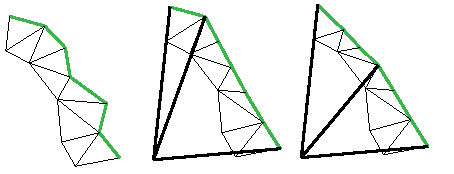
\includegraphics{curve_meshing_in_shell_tex/figs/slide_on_feature.pdf}
    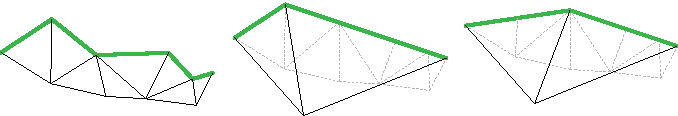
\includegraphics[width=\linewidth]{curve_meshing_in_shell_tex/figs/illustrations/loc-op.pdf}
    \caption{Illustration of smoothing on a feature.}
    \label{bichon:fig:loc-op}
\end{figure}

To construct a mesh $\overline\M$ with straight features, 
we start with $\overline\M = \M$ (in the beginning all prisms of $\PS$ cover at most one feature edge).
Let $\overline f^1 = \{\overline f_i^1\}, i=1,\dots,n$ and $\overline f^2 = \{\overline f_i^2\}, i=1,\dots,k$ two chains of {feature} edge belonging to the same feature $\overline f \in \overline\F$.
For every local operation acting on a feature $\overline f_1$ and $\overline f_2$  we first construct the new feature $\overline f^n = \{\overline f_i^n\}, i=1,\dots,k$ such that the segments $(\overline f_i^n, \overline f_{i+1}^n)$ are collinear and their length is proportional to $( f_i, f_{i+1})$ (the feature vertices in the input mesh $\M$), that this we use arc-length cross parameterization from $f$ to $\overline f^n$ (Figure~\ref{bichon:fig:loc-op} show an example of smoothing a feature). Moving vertices of $\overline f^n$ will also move the vertices of $\overline\M$ thus, straighten the mesh as the local operations {proceed}. After the construction of $\overline f^n$ we check if the newly constructed $\overline\M$ is still a section of $\PS$ and if the triangles modified by the straightening have {areas} larger than  $\epsilon$. In practice, we choose $\epsilon=10^{-10}$: a smaller value would lead to numerical instabilities and a larger one to less straightening.

Note that not all features can be {straight}; for instance, if a triangle has three feature vertices (the snapped feature will result {in} a degenerate triangle, thus, $\beta$ will not be bijective) or if the snapping flips the normal ($\overline\M$ will no longer be a section of $\PS$). Both are extremely rare cases in our dataset.
%%%%%%%%%%%%%%%%%%%%%%%%%%%%%%%%%%%%%%%%%%%%%%


\section{Results}

{Our} algorithm is implemented in C++, {using} Eigen \cite{eigenweb} for the linear algebra routines, CGAL \cite{cgal2008computational} and Geogram \cite{levy2015geogram} for predicates and geometric kernel, libigl \cite{jacobson2016libigl} for basic geometry processing routines, and
meshio \cite{schlomer2020nschloe} for converting across the different formats.
We run our experiments on cluster nodes with Intel Xeon Platinum 8268 CPU 2.90GHz.
The reference implementation and the data used to generate the results will be released as an open-source project.


\begin{figure}
    \centering\small
    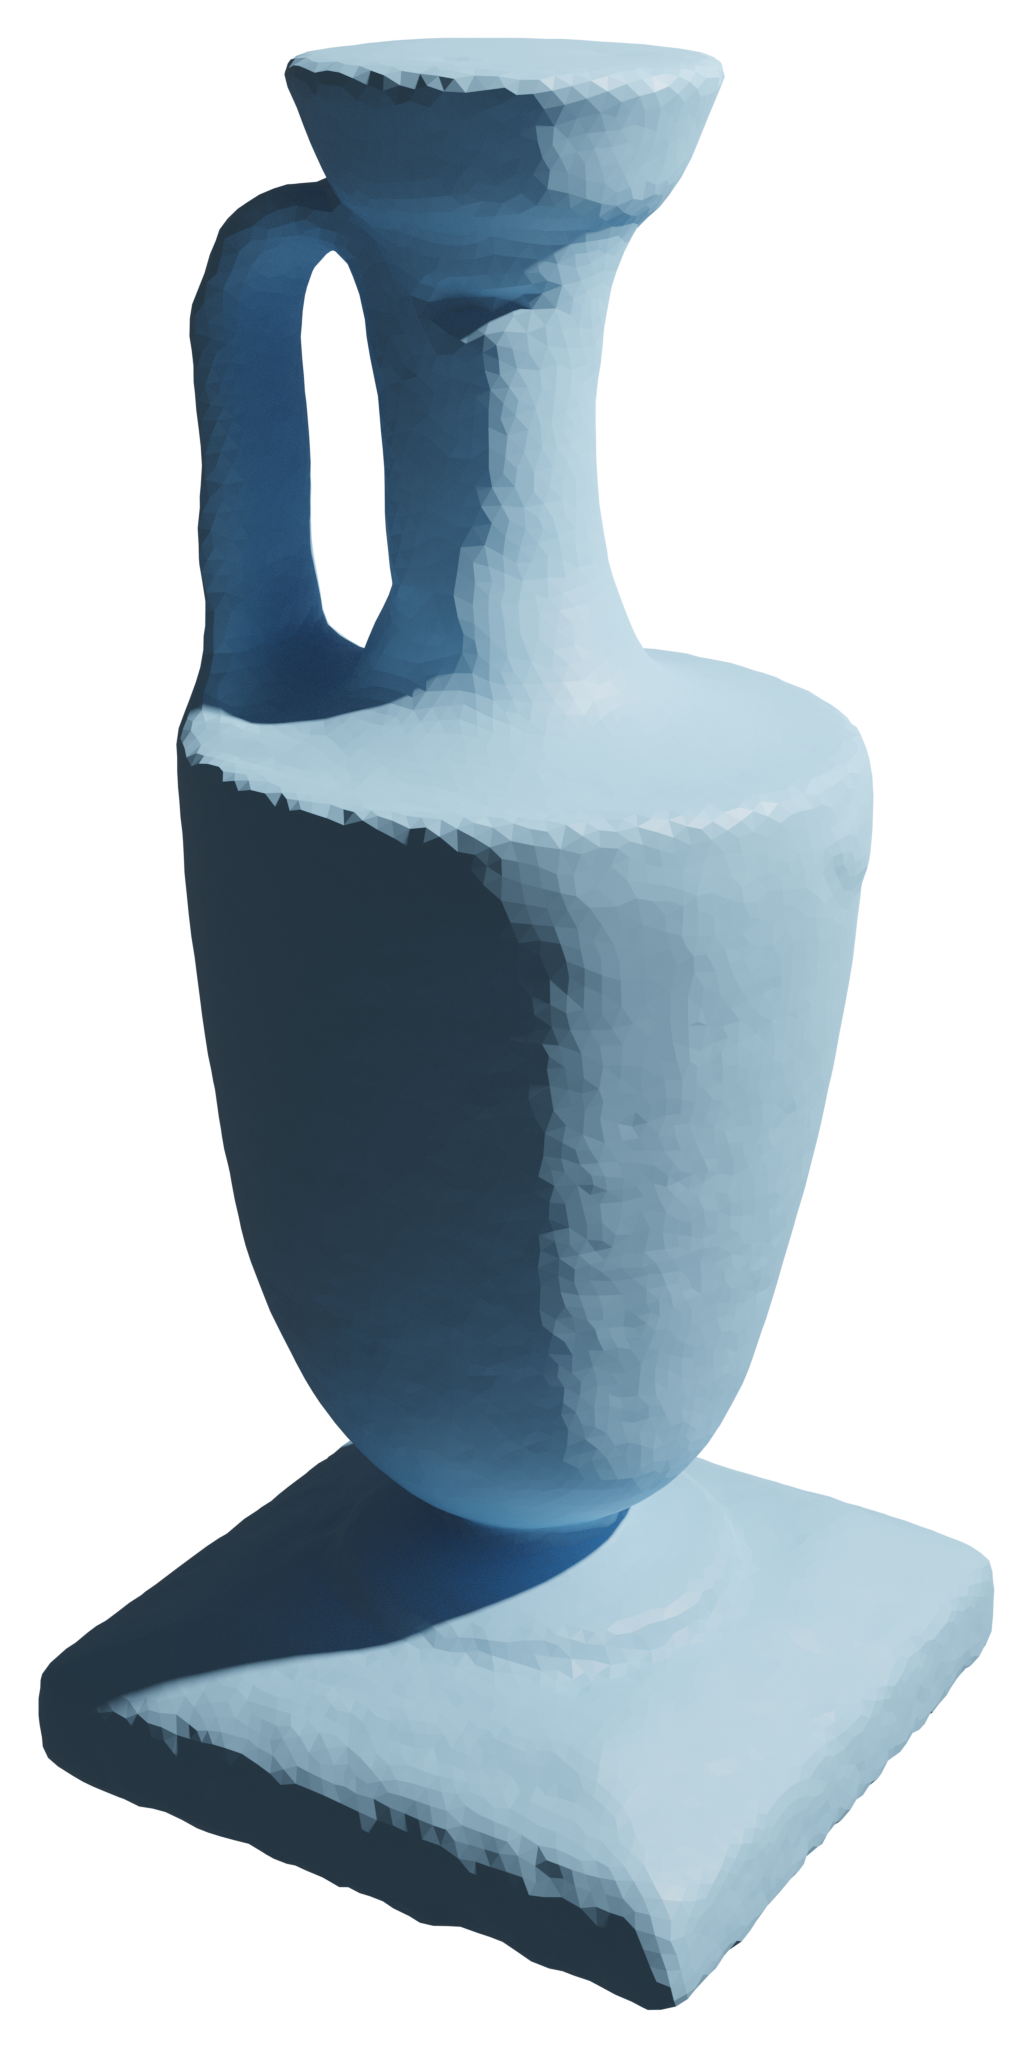
\includegraphics[width=.23\linewidth]{curve_meshing_in_shell_tex/figs/anphora/0005}
    \hfill
    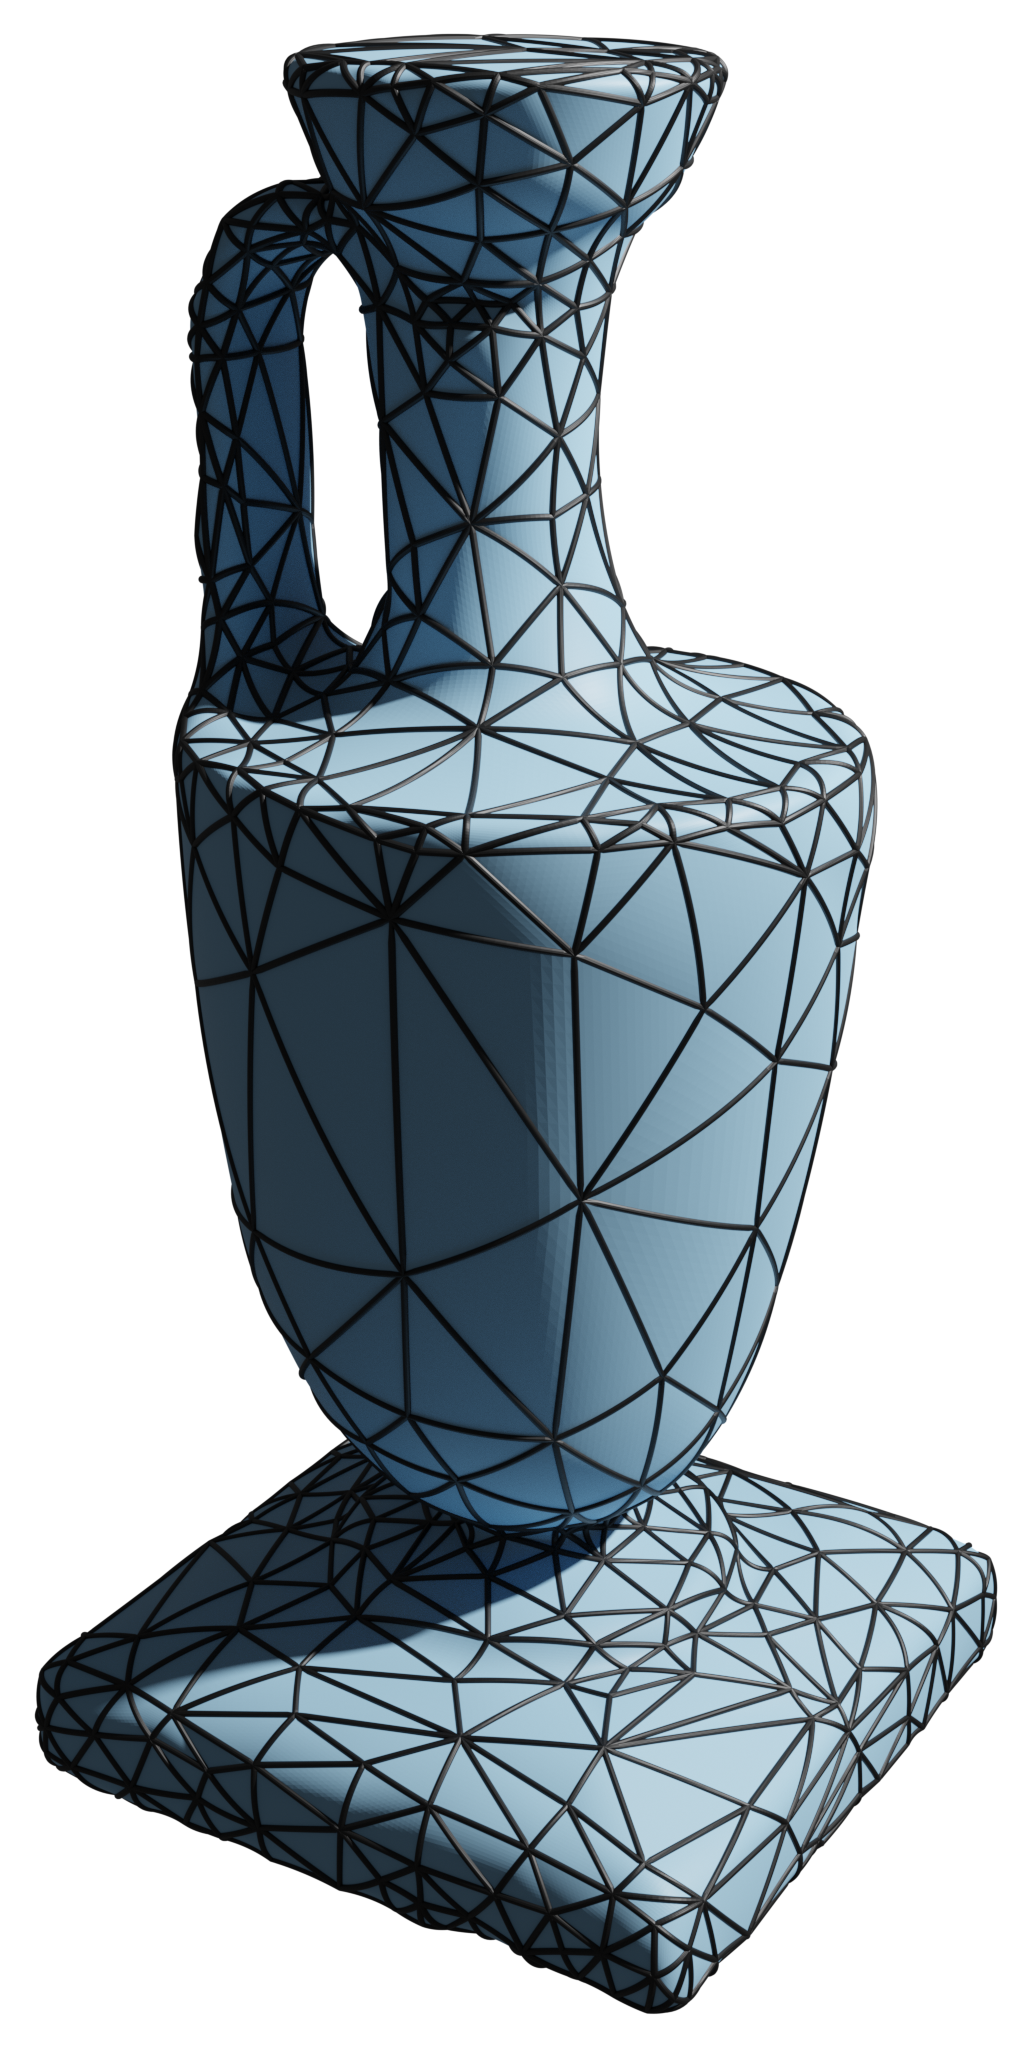
\includegraphics[width=.23\linewidth]{curve_meshing_in_shell_tex/figs/anphora/0001}\hfill
    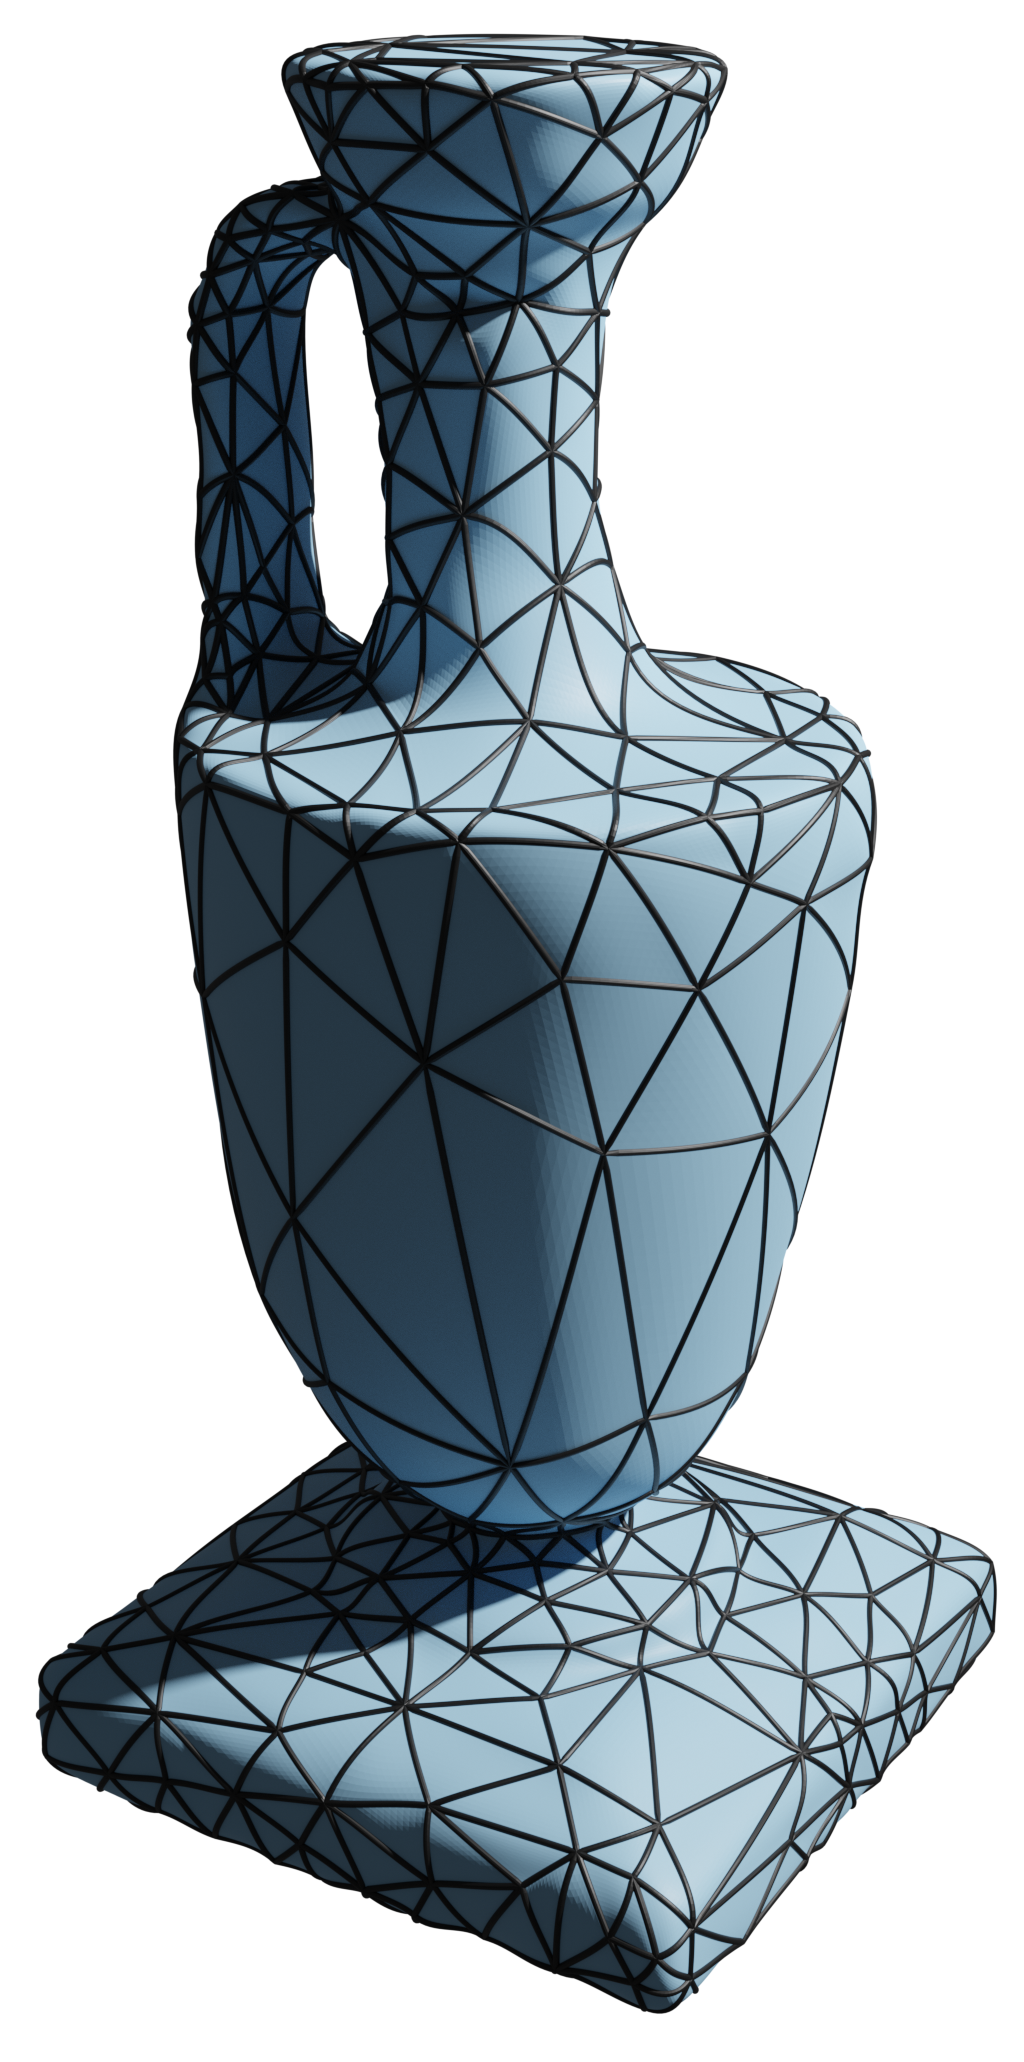
\includegraphics[width=.23\linewidth]{curve_meshing_in_shell_tex/figs/anphora/0002}\hfill
    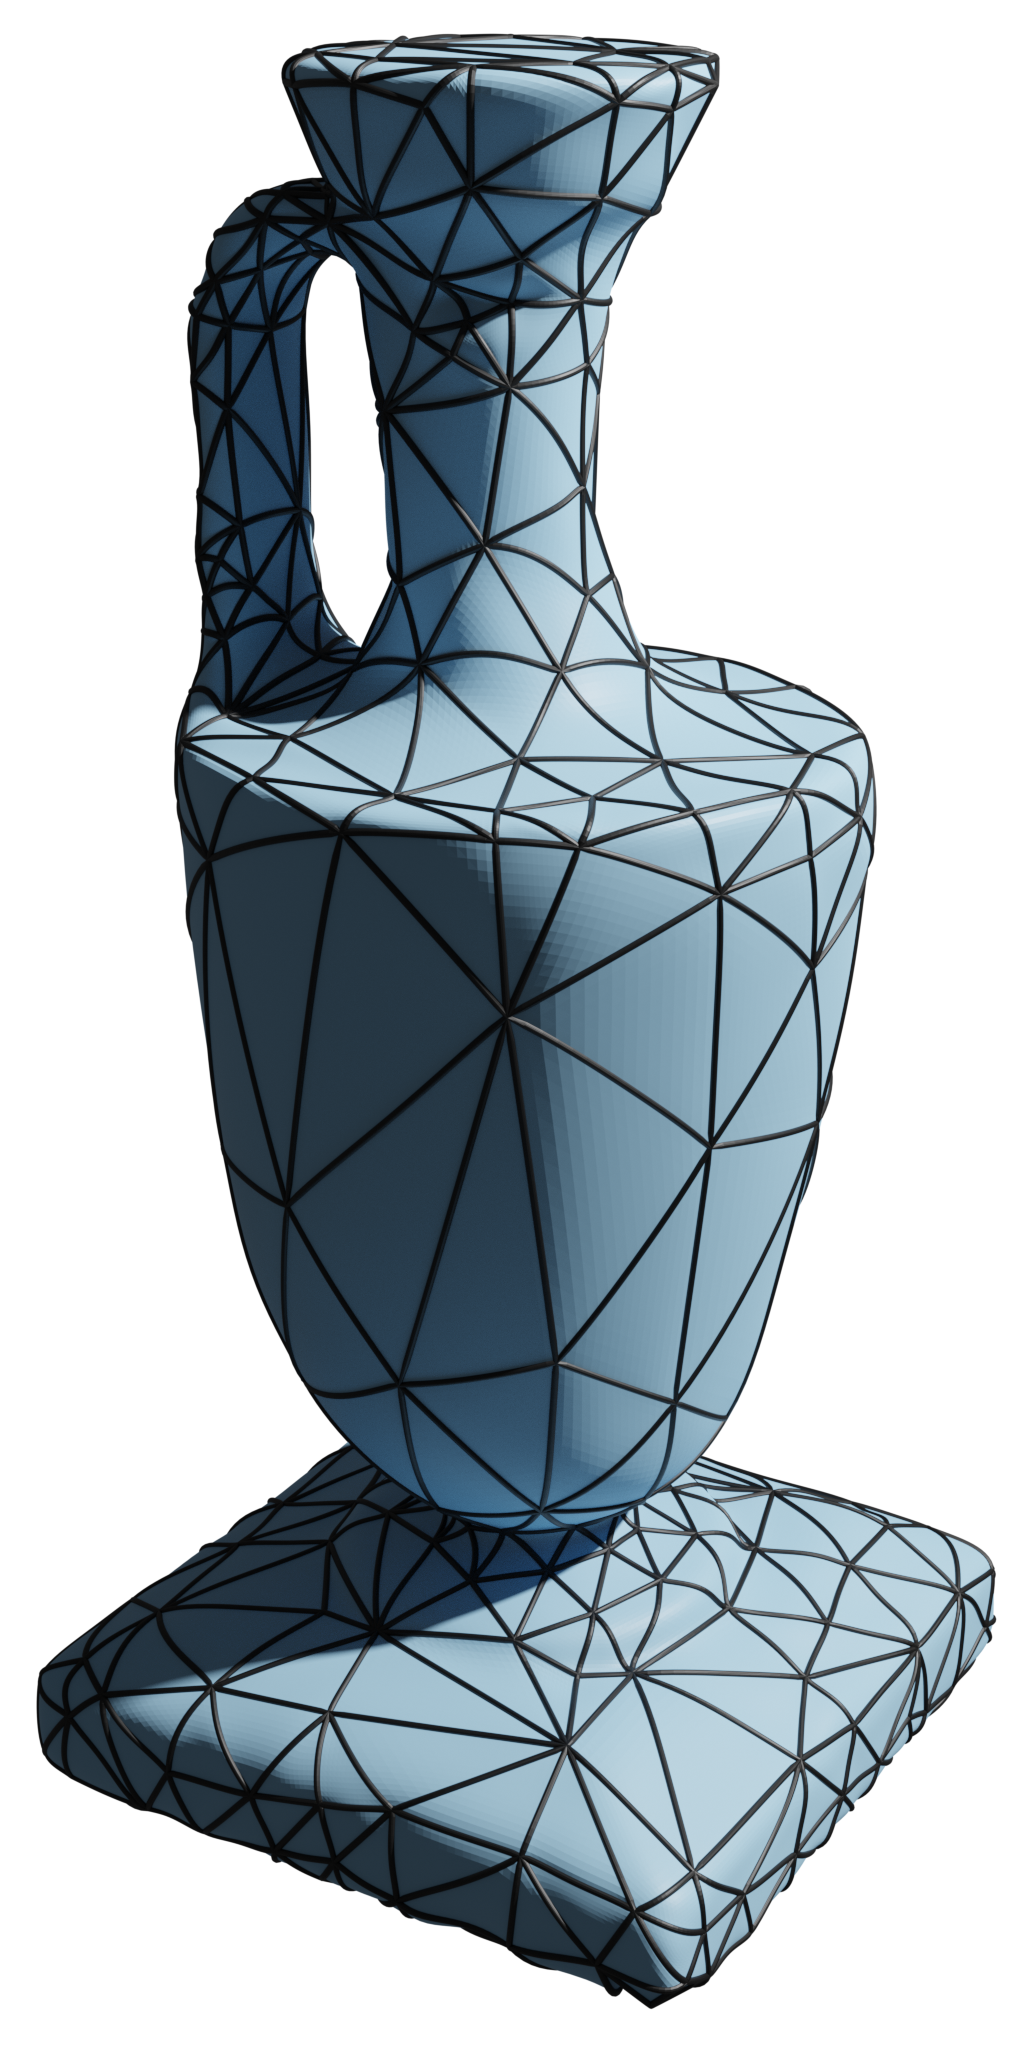
\includegraphics[width=.23\linewidth]{curve_meshing_in_shell_tex/figs/anphora/0003}
     \parbox{.24\linewidth}{\centering Input}\hfill
    \parbox{.24\linewidth}{\centering $k=3$}\hfill
    \parbox{.24\linewidth}{\centering $k=4$}\hfill
    \parbox{.24\linewidth}{\centering $k=5$}
    \caption{Curved meshes of different order. The additional degrees of freedom allows for more coarsening.}
    \label{bichon:fig:diff-k}
\end{figure}

To simplify the exposition, all meshes presented in this section are quartic meshes ($k=4$). Our method is flexible and, for lower $k$, it will generate denser meshes (Figure~\ref{bichon:fig:diff-k}).

\subsection{Large Scale Validation.}

We tested the robustness and quality of the result produced by our algorithm on three datasets: (1) Thingi10k dataset \cite{zhou2016thingi10k} containing 3574 models without features; (2) the first chunk {of} the ABC dataset~\cite{koch2019abc} with 5328 models with features marked from the STEP file and (3) the CAD dataset~\cite{Gao:2019} containing 106 models with semi-manual features.
%\ZJ{47 Thingi, 60 ABC out-of-time 12 hours}

Note that the original datasets contain more models since, for each of them, we selected meshes satisfying our assumptions: intersection-free (using the same strategy as in~\ref{chp:shell} with a distance tolerance of $10^{-6}$ and dihedral angle of $2^\circ$) oriented, manifold triangle meshes, smallest triangle area larger than $10^{-8}$. 





\begin{figure}
    \centering
    % \includegraphics{}
    \parbox{0.02\linewidth}{~}\hfill\hfill
    \parbox{.3\linewidth}{\centering Thingi10k}\hfill
    \parbox{.3\linewidth}{\centering ABC}\hfill
    \parbox{.3\linewidth}{\centering CAD}\par
    %
    \parbox{0.02\linewidth}{\centering\rotatebox{90}{\scriptsize{Edge length \%}}}\hfill\hfill
    \parbox{.3\linewidth}{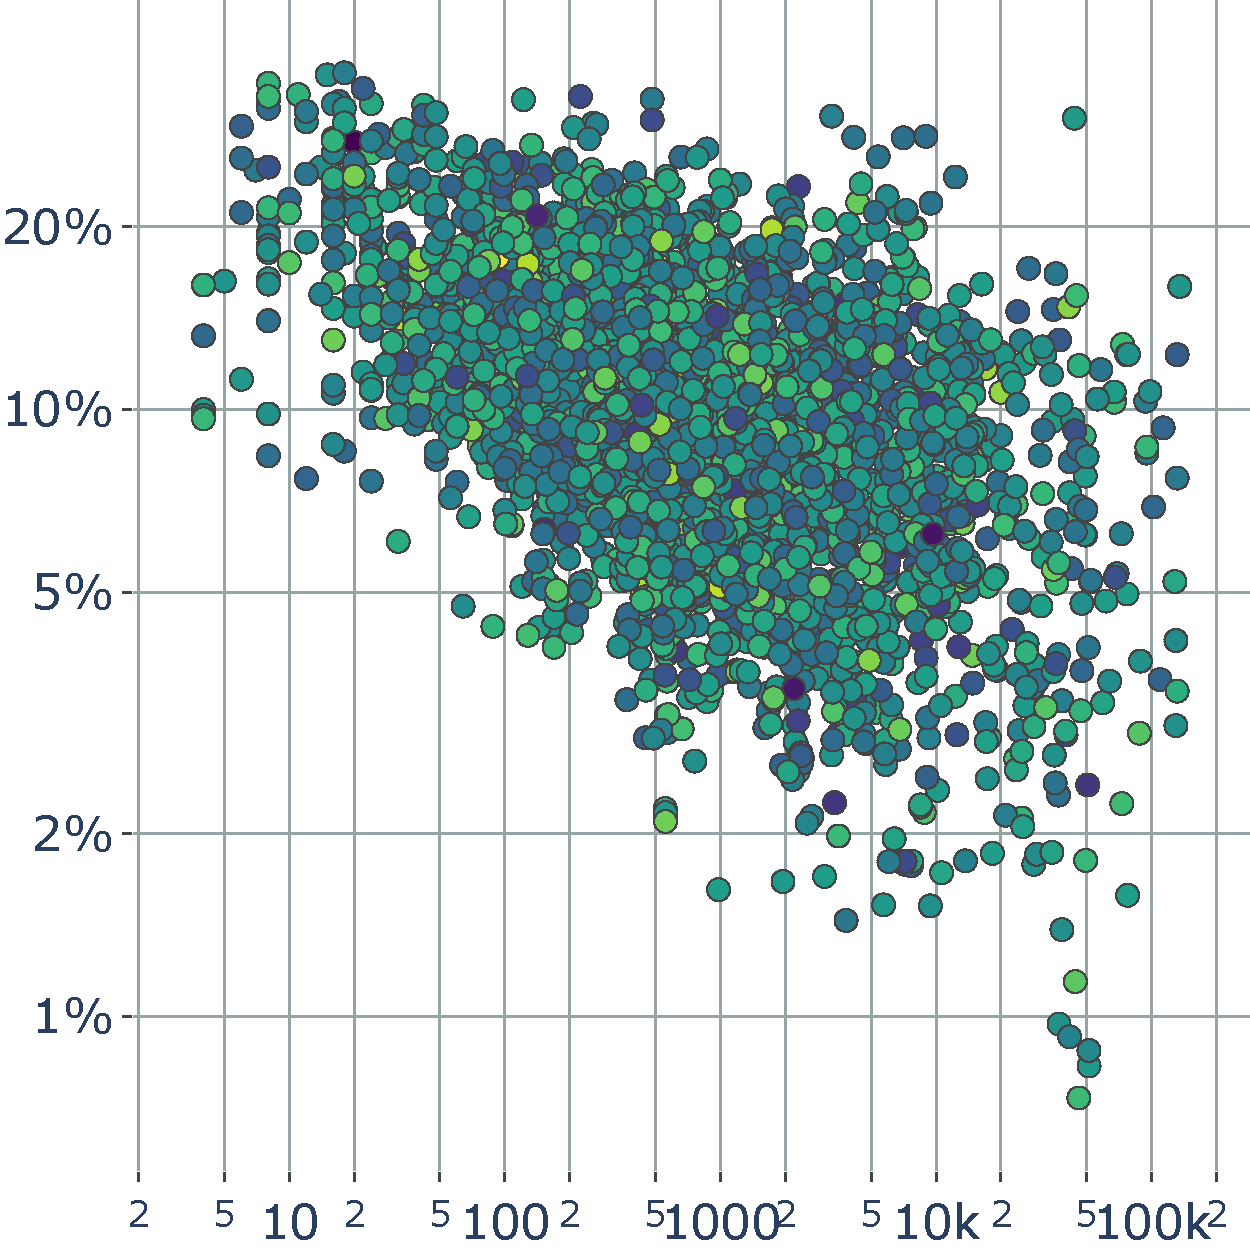
\includegraphics[width=\linewidth]{curve_meshing_in_shell_tex/figs/stats/edgelength_Thingi10k}}\hfill
    \parbox{.3\linewidth}{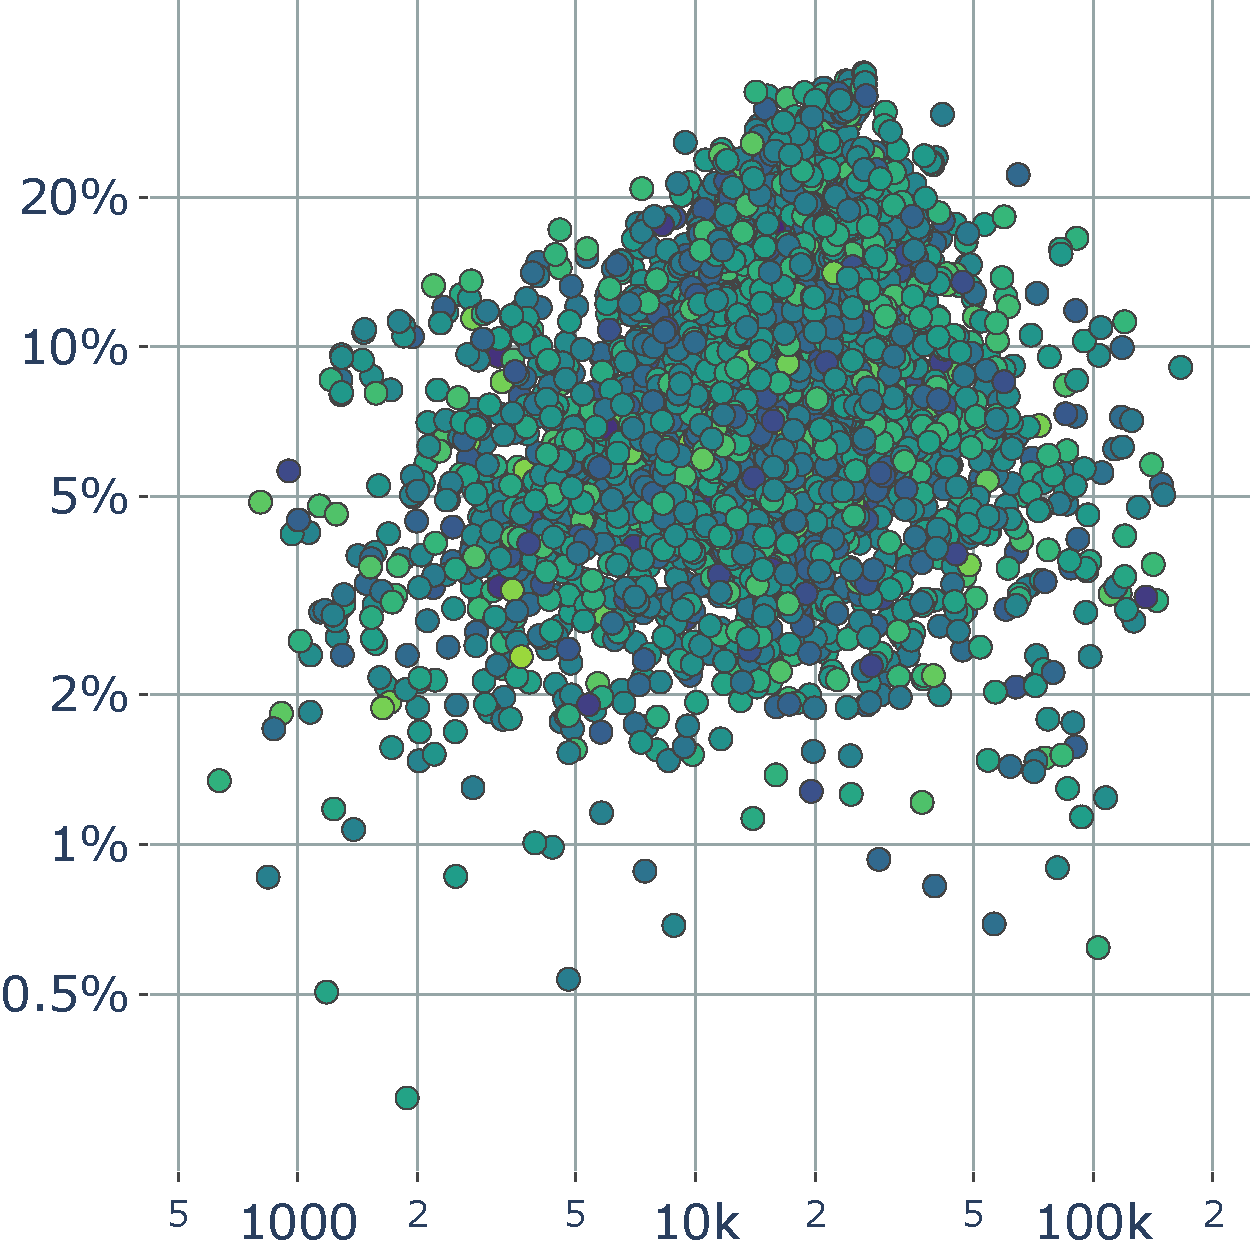
\includegraphics[width=\linewidth]{curve_meshing_in_shell_tex/figs/stats/edgelength_ABC}}\hfill
    \parbox{.3\linewidth}{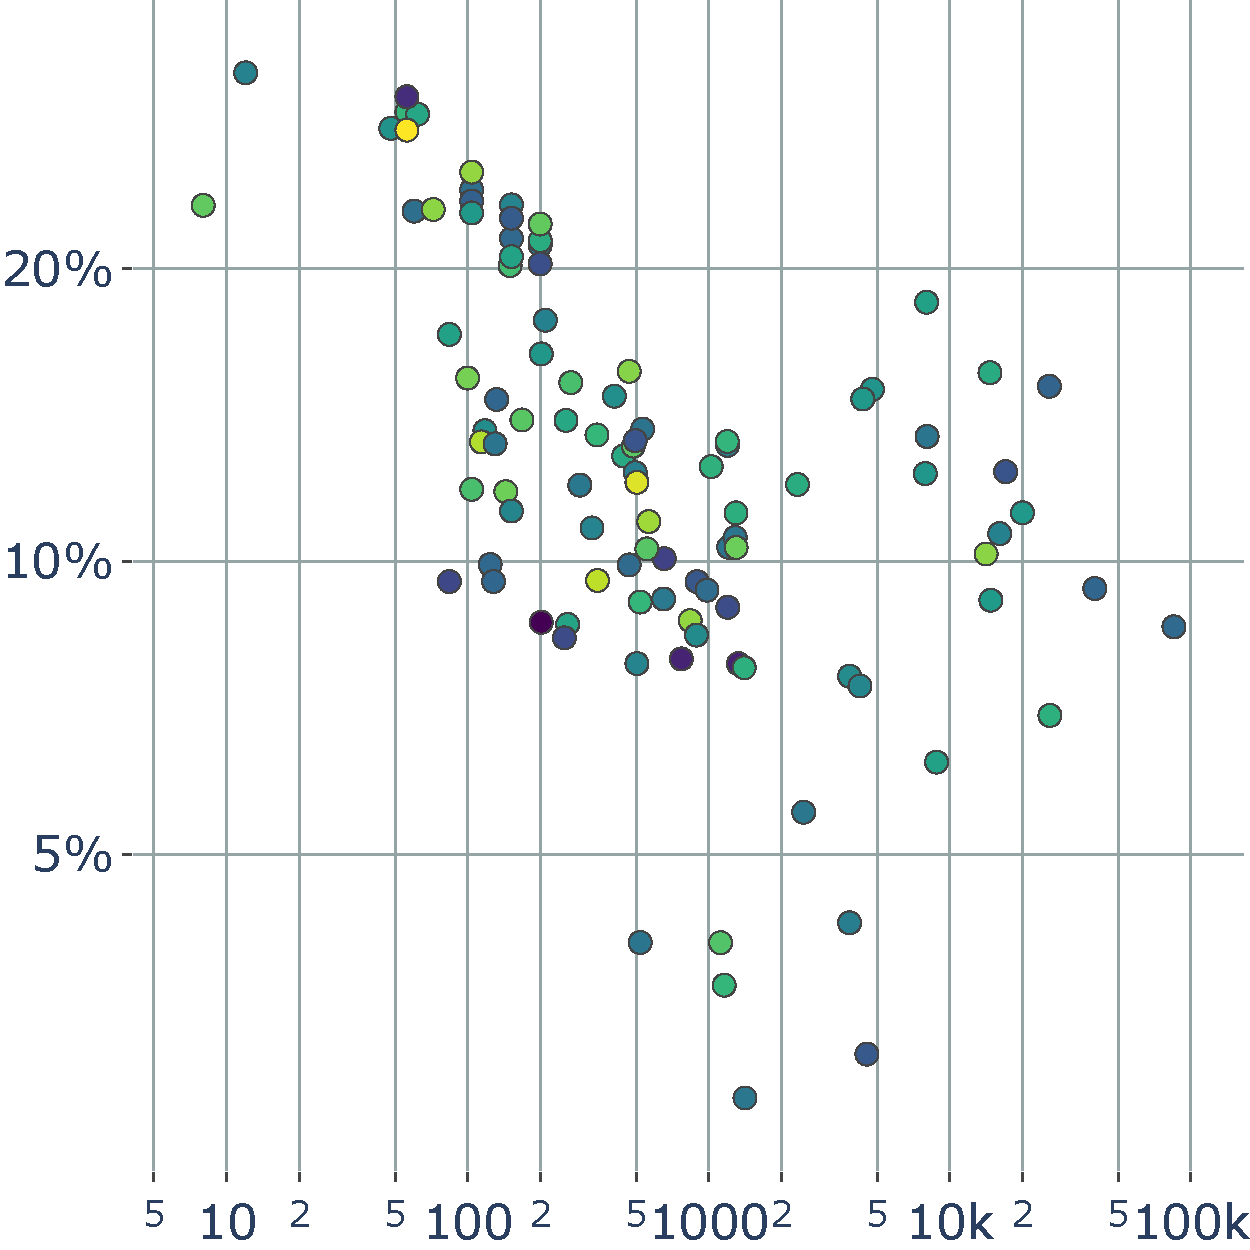
\includegraphics[width=\linewidth]{curve_meshing_in_shell_tex/figs/stats/edgelength_PolyCube}}\par
    \scriptsize{Input Vertices}
    \caption{Relative average edge length (with respect to longest bounding box edge of each model) of our curved meshes versus number of input vertices.}
    \label{bichon:fig:tet-count}
\end{figure}


\begin{figure}
    \centering\small
    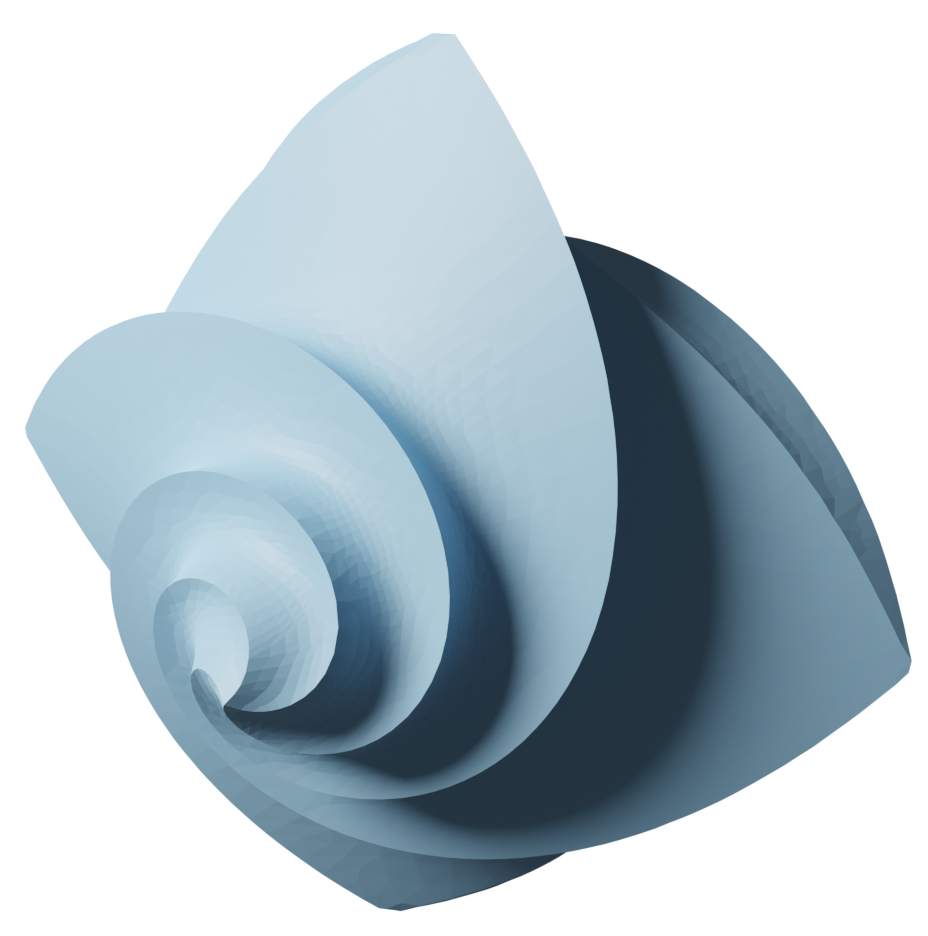
\includegraphics[width=.32\linewidth]{curve_meshing_in_shell_tex/figs/octa/0003}\hfill
    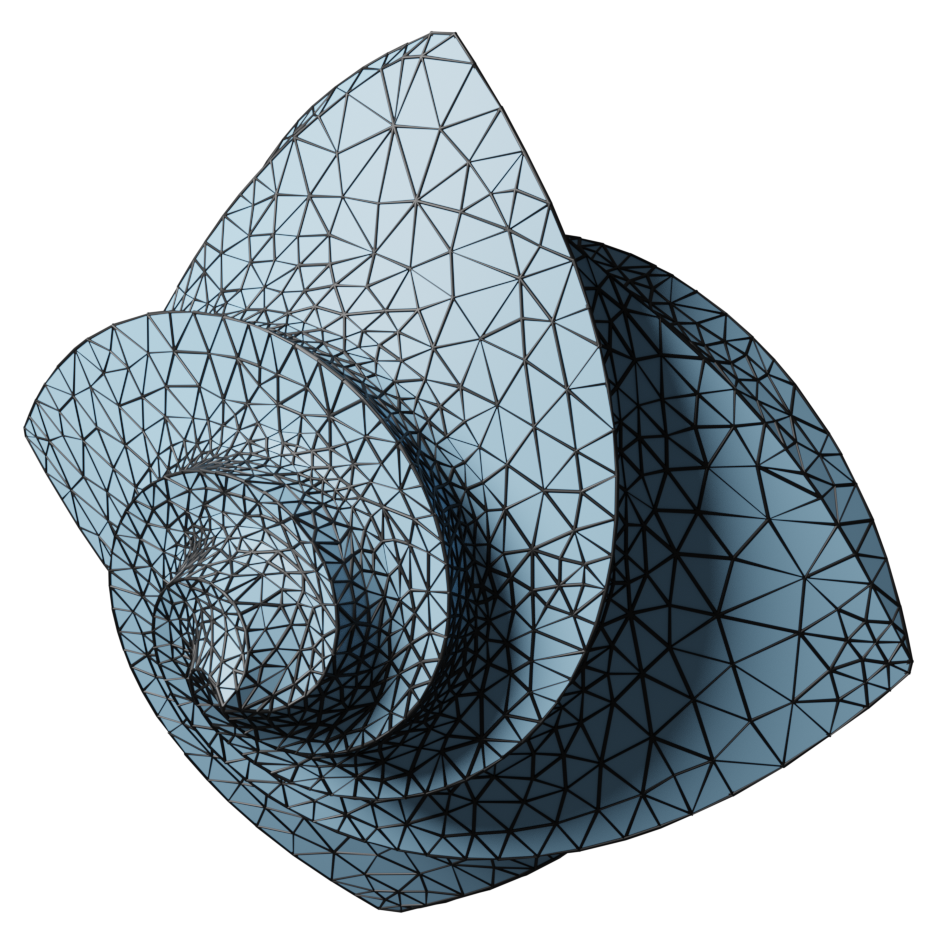
\includegraphics[width=.32\linewidth]{curve_meshing_in_shell_tex/figs/octa/0002}\hfill
    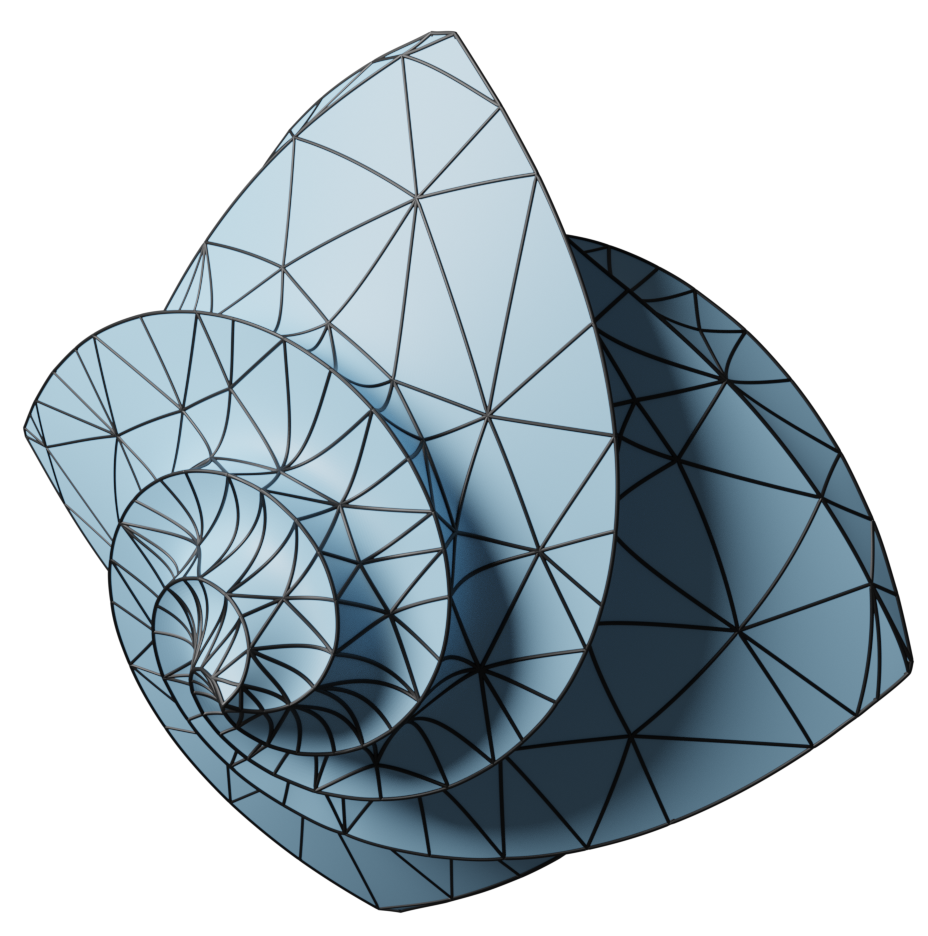
\includegraphics[width=.32\linewidth]{curve_meshing_in_shell_tex/figs/octa/0001}\par
    \parbox{.32\linewidth}{\centering Input}\hfill
    \parbox{.32\linewidth}{\centering fTetWild}\hfill
    \parbox{.32\linewidth}{\centering Ours}
    \caption{Within the same distance bound ($10^{-3}$ of the longest bounding box side), our method generates a coarser high order mesh, compared to the linear counterpart generated by fTetWild.}
    \label{bichon:fig:us-vs-ftetwild}
\end{figure}

Our method has only the geometry accuracy parameter $\varepsilon$, which we set to $1\%$ {of the longest bounding box edge}, and the point set $\P$ which we set {as} the input vertices $V$. 
With this basic setup, our algorithm aims to produce the coarsest possible mesh while preserving features and striving to generate high-quality meshes.
Our algorithm successfully generates curved meshes for 3527 for Thingi10k, 5268 for the ABC, and all for CAD dataset within 12 {hours}; by allowing more time, all models but 3 can be successfully processed. 
The 3 failures are due to models with a small one-tetrahedra component {that} ``move'' inside the shell as it grows. This is an implementation choice: we use collision detection instead of continuous collision detection for efficiency reasons.

Our method successfully {generates} coarse meshes whose average edge length is 10\% of the model size while preserving features (Figure~\ref{bichon:fig:tet-count}).
Figure~\ref{bichon:fig:us-vs-ftetwild} shows how our method successfully {captures} the features and coarsen the surface with curved elements, while many linear elements (generated with fTetWild~\cite{Hu:2020:fTetWild}) are required to closely approximate the surface.


\begin{figure}
    \centering
    % \includegraphics{}
    \parbox{0.02\linewidth}{~}\hfill\hfill
    \parbox{.3\linewidth}{\centering Thingi10k}\hfill
    \parbox{.3\linewidth}{\centering ABC}\hfill
    \parbox{.3\linewidth}{\centering CAD}\par
    %
    \parbox{0.02\linewidth}{\centering\rotatebox{90}{\scriptsize{Volume energy}}}\hfill\hfill
    \parbox{.3\linewidth}{\includegraphics[width=\linewidth]{curve_meshing_in_shell_tex/figs/stats/energy_Thingi10k}}\hfill
    \parbox{.3\linewidth}{\includegraphics[width=\linewidth]{curve_meshing_in_shell_tex/figs/stats/energy_ABC}}\hfill
    \parbox{.3\linewidth}{\includegraphics[width=\linewidth]{curve_meshing_in_shell_tex/figs/stats/energy_PoLyCube}}\par
    \scriptsize{Surface Energy}
    \caption{Surface and volume average MIPS energy of the output of our method (the CAD volume energy is truncated at 100, excluding 6 models).}
    \label{bichon:fig:quality}
\end{figure}

The output of our algorithm can be directly used in {the} simulation (Section~\ref{cumin:sec:application}) since we guarantee that the geometric mapping $g$ is positive. To ensure good conditioning and performance of the numerical solver, we measure the MIPS energy~\cite{hormann2000mips,fu2015computing} of our output meshes (Figure~\ref{bichon:fig:quality}). 

\begin{figure}
    \centering
    % \includegraphics{}
    \parbox{0.02\linewidth}{~}\hfill\hfill
    \parbox{.3\linewidth}{\centering Thingi10k}\hfill
    \parbox{.3\linewidth}{\centering ABC}\hfill
    \parbox{.3\linewidth}{\centering CAD}\par
    %
    \parbox{0.02\linewidth}{\centering\rotatebox{90}{\scriptsize{Time(s)}}}\hfill\hfill
    \parbox{.3\linewidth}{\includegraphics[width=\linewidth]{curve_meshing_in_shell_tex/figs/stats/time_Thingi10k}}\hfill
    \parbox{.3\linewidth}{\includegraphics[width=\linewidth]{curve_meshing_in_shell_tex/figs/stats/time_ABC}}\hfill
    \parbox{.3\linewidth}{\includegraphics[width=\linewidth]{curve_meshing_in_shell_tex/figs/stats/time_PoLyCube}}\par
    \scriptsize{Input Vertices}
    \caption{Timing of our algorithm versus the input number of vertices.}
    \label{bichon:fig:timings}
\end{figure}

Figure~\ref{bichon:fig:timings} shows the running time of our method with respect to the number of vertices. The running time of our algorithm is linear with respect to the number of input vertices; it takes around an hour for a model with around 10 thousand vertices.


%%%%%%%%%%%%%%%%%%%%%%%%%%%%%%%%%%%%%%%%%%%%%%%%%%%%%%%%%%%%%%%%%%%
%%%%%%%%%%%%%%%%%%%%%%%%%%%%%%%%%%%%%%%%%%%%%%%%%%%%%%%%%%%%%%%%%%%
\subsection{Comparisons}\label{cumin:sec:comparison}



\paragraph{Curved ODT}
\cite{feng2018curved} is, to the best of our knowledge, the only existing algorithm designed to convert dense triangle meshes into coarse, curved approximations. The input and output are the same as in our algorithm. However, their method does not provide a bijective map between the input and output, does not guarantee to preserve features, has no bound on the distance to the input surface, and does not guarantee that the elements are positive. While our algorithm has been designed to process large collections of data automatically, exposing only a few intuitive options to control the faithfulness to the input, the reference implementation of the curved ODT method provided to us by the authors requires the user to choose multiple \emph{per-model} parameters to achieve good results, and the parameters have a strong effect on the quality and validity of the result (as shown in~\cite[Figure 16]{feng2018curved}). We thus restricted our comparison to only a small selection of models (see additional material) that the authors of \cite{feng2018curved} processed for us.
%
\begin{figure}
    \centering\small
    \includegraphics[width=.24\linewidth]{curve_meshing_in_shell_tex/figs/gargo/0001}\hfill
    \includegraphics[width=.24\linewidth]{curve_meshing_in_shell_tex/figs/gargo/0002}\hfill
    \includegraphics[width=.24\linewidth]{curve_meshing_in_shell_tex/figs/gargo/0003}\hfill
    \includegraphics[width=.24\linewidth]{curve_meshing_in_shell_tex/figs/gargo/0004}
    \parbox{.24\linewidth}{\centering Input}\hfill
    \parbox{.24\linewidth}{\centering CODT with uniform\\(46249 elements)}\hfill
    \parbox{.24\linewidth}{\centering CODT with LFS\\(38159 elements)}\hfill
    \parbox{.24\linewidth}{\centering Our\\(2037 elements)}\par
    \caption{Compared with Curved ODT, our method does not rely on setting vertex number and sizing field, and can generate coarse valid results.}
    \label{bichon:fig:cdt}
\end{figure}

From our discussions with the authors, we observed that curved ODT generates a \emph{valid} output when we provide (1) a sufficiently large number of vertices and (2) a good local feature size sizing field (LFS)~\cite{alliez2005variational} to efficiently spend the vertex budget in the regions with more geometrical details.  Figure~\ref{bichon:fig:cdt} shows an example of a model for which \cite{feng2018curved} fails to converge when using a uniform sizing field, while it succeeds when the sizing field is used.

In contrast, our algorithm can be run automatically on {a} large collection of geometrical models, it is guaranteed to have positive Jacobian (up to the use of floating-point predicates, Section~\ref{cumin:sec:conclusion}), it preserves features, it automatically controls the density of the output depending on the desired user-provided distance threshold, and it provides a bijective map between the input mesh the boundary of the curved surface. For the model in Figure \ref{bichon:fig:cdt}, our result contains 2037 elements, 18 times less than the curved ODT algorithm. %We note that the LFSSF is brittle and the authors were unable to generate it for complex models with features (see additional material), thus their algorithm fails.


\begin{figure}
    \centering\small
    \includegraphics[width=0.32\linewidth]{curve_meshing_in_shell_tex/figs/gmsh/not-bij}\hfill
    \includegraphics[width=0.32\linewidth]{curve_meshing_in_shell_tex/figs/gmsh/bij}\hfill
    \includegraphics[width=0.32\linewidth]{curve_meshing_in_shell_tex/figs/gmsh/torus}
     \parbox{.32\linewidth}{\centering Gmsh Fixed Surface}\hfill
    \parbox{.32\linewidth}{\centering Gmsh Free Surface}\hfill
    \parbox{.32\linewidth}{\centering Ours}\par
    \caption{Example of a BRep meshed with Gmsh where the optimization fails to untangle elements when fixing the surface. By allowing the surface to be modified, the mesh becomes ``wiggly''. Our method successfully generate a positive curved mesh.}
    \label{bichon:fig:gmsh-flipped}
\end{figure}


\begin{figure}
    \centering\small
    \includegraphics[width=.32\linewidth]{curve_meshing_in_shell_tex/figs/gmsh/step/0001}\hfill
    \includegraphics[width=.32\linewidth]{curve_meshing_in_shell_tex/figs/gmsh/step/0002}\hfill
    \includegraphics[width=.32\linewidth]{curve_meshing_in_shell_tex/figs/gmsh/step/0003}\par
    \parbox{.32\linewidth}{\centering Coarse Gmsh}\hfill
    \parbox{.32\linewidth}{\centering Dense Gmsh}\hfill
    \parbox{.32\linewidth}{\centering Ours}\par
    \caption{Example of a STEP file meshed with Gmsh where, due to the low mesh density, the tetrahedralization is not positive. Gmsh manages to generate a positive mesh by using a denser initial  tessellation. Since our method starts from a dense mesh and coarsen it, it can successfully resolve the geometry.}
    \label{bichon:fig:closed-holes}
\end{figure}
\paragraph{Gmsh}
\cite{Geuzaine:2009:gmsh} can only generate curved meshes from boundary representation (BRep), that is the input is not exactly the same as ours. To compare both algorithms, we start from the BRep and we generate a dense \emph{linear} mesh that we use for our input. The Gmsh algorithm {first} constructs a curved mesh by fitting the high-order nodes to the BRep (possibly inverting elements) then performs mesh optimization to untangle them~\cite{remacle2013robust}; thus has no guarantee to generate positive meshes while preserving the surface (Figure~\ref{bichon:fig:gmsh-flipped}, left). Additionally, Gmsh algorithm cannot control the distance from the input when the untangling allows the surface to move, and thus the surface is ``wiggly'' and denser than our result (Figure~\ref{bichon:fig:gmsh-flipped}, center). We also observed that if the initial surface mesh is not dense enough, Gmsh closes holes and cannot generate a valid tetrahedral mesh (Figure~\ref{bichon:fig:closed-holes}).


%%%%%%%%%%%%%%%%%%%%%%%%%%%%%%%%%%%%%%%%%%%%%%%%%%%%%%%%%%%%%%%%%%%
%%%%%%%%%%%%%%%%%%%%%%%%%%%%%%%%%%%%%%%%%%%%%%%%%%%%%%%%%%%%%%%%%%%
\subsection{Flexibility}

\begin{figure}
    \centering\small
    %\includegraphics[width=0.45\linewidth]{curve_meshing_in_shell_tex/figs/micro/0001}\hfill
    \includegraphics[width=0.49\linewidth]{curve_meshing_in_shell_tex/figs/micro/color}\hfill
    %\includegraphics[width=0.45\linewidth]{curve_meshing_in_shell_tex/figs/spot.png}\hfill
    \includegraphics[width=0.49\linewidth]{curve_meshing_in_shell_tex/figs/spot.png}\par
    \parbox{.49\linewidth}{\centering Implicit microstructure}\hfill
    \parbox{.49\linewidth}{\centering {subdivision} surface}
    \caption{Our algorithm processes triangle meshes that can be extracted from different formats: an implicit  microstructure geometry from \cite{tozoni2020low} or a subdivision surface from  \cite{crane2013conformal}. The bijective map preserved on the surface allows taking advantage of the plethora of surface algorithms including polyhedral geodesic computation \cite{mitchell1987discrete} and texture mapping.}
    \label{bichon:fig:flex}
\end{figure}

Since the input to our method is a triangle mesh, our method naturally supports a variety of input that can be easily converted into triangle meshes. For instance, $\M$ can be {generated from} marching an implicit surface or Catmull-Clark subdivision of a hand-made quad mesh (Figure~\ref{bichon:fig:flex}). The bijective map $\phi^k$ {is used}, for instance, to transfer the geodesic distance field or color information from the input triangle mesh to the coarse curved mesh.


%%%%%%%%%%%%%%%%%%%%%%%%%%%%%%%%%%%%%%%%%%%%%%%%%%%%%%%%%%%%%%%%%%%
%%%%%%%%%%%%%%%%%%%%%%%%%%%%%%%%%%%%%%%%%%%%%%%%%%%%%%%%%%%%%%%%%%%
\subsection{Applications}\label{cumin:sec:application}


\begin{figure}
    \centering
    % \includegraphics{}
    \parbox{0.01\linewidth}{~}\hfill\hfill
    \parbox{.3\linewidth}{\centering Thingi10k}\hfill
    \parbox{.3\linewidth}{\centering ABC}\hfill
    \parbox{.3\linewidth}{\centering CAD}\par
    %
    \parbox{0.01\linewidth}{\centering\rotatebox{90}{\scriptsize{$L^2$ error}}}\hfill\hfill
    \parbox{.3\linewidth}{\includegraphics[width=\linewidth]{curve_meshing_in_shell_tex/figs/stats/error_Thingi10k}}\hfill
    \parbox{.3\linewidth}{\includegraphics[width=\linewidth]{curve_meshing_in_shell_tex/figs/stats/error_ABC}}\hfill
    \parbox{.3\linewidth}{\includegraphics[width=\linewidth]{curve_meshing_in_shell_tex/figs/stats/error_PolyCube}}\par
    \scriptsize{Average Edge Length}
    \caption{$L^2$ error of the solution of the Poisson equation with respect to model size on our three datasets.}
    \label{bichon:fig:large-scale-poisson}
\end{figure}

\paragraph{Large Scale Poisson}
To show that our meshes are ready for simulation, we solve for Poisson equation
\[
\Delta u  = f,\quad
u|_{\partial \Omega} = g,
\]
where $\Omega$ is the domain (i.e., the mesh), $f$ is the right-hand side, and $g$ are the Dirichlet boundary conditions. To simplify the setup and the error measurements, we use fabricated solutions~\cite{SALARI:2000:CVB}. That is, we choose the function $u_\text{exact}$ to be {%\scriptsize
\begin{align*}
u_\text{exact}&(x_1,x_2,x_3) =
\\&3/4\,{ e}^{-((9x_1-2)^2+(9x_2-2)^2+(9x_3-2)^2)/4}+
3/4\,{ e}^{-(9x_1+1)^2/49-(9x_2+1)/10-(9x_3+1)/10} \\
%
&+1/2\,{ e}^{-((9x_1-7)^2+(9x_2-3)^2+(9x_3-5)^2)/4}-
1/5\,{ e}^{-(9x_1-4)^2-(9x_2-7)^2-(9x_3-5)^2},
\end{align*}}
then we plug it in the equation to obtain $f$ ($g$ is simply $u_\text{exact}$). Figure~\ref{bichon:fig:large-scale-poisson} shows the $L^2$ error (average) distribution across our three datasets using our quartic meshes with quadratic approximation of $u$ (i.e., we use superparametric elements).


\begin{figure}
    \centering\small
    % \includegraphics[width=.32\linewidth]{curve_meshing_in_shell_tex/figs/fluid/0001}\hfill
    \includegraphics[width=.45\linewidth]{curve_meshing_in_shell_tex/figs/fluid/0003}\hfill
    \includegraphics[width=.53\linewidth]{curve_meshing_in_shell_tex/figs/fluid/0002}\hfill
    % \includegraphics[width=.32\linewidth]{curve_meshing_in_shell_tex/figs/fluid/0001}\par
    \parbox{.45\linewidth}{\centering Tetrahedral mesh}\hfill
    \parbox{.53\linewidth}{\centering Curved simulation}\hfill
    % \parbox{.32\linewidth}{\centering Linear simulation}
    \caption{By meshing the region between a box and a complicated obstacle, we are able to perform non-linear fluid simulation on our curved mesh.}
    \label{bichon:fig:ns}
\end{figure}
\paragraph{High Accuracy Fluids}
Our curved meshes can be directly used to solve different partial differential equations (PDEs). For instance, by meshing the part outside the top shell and discarding the rest, we can generate a curved background mesh for the Navier-Stokes equation (Figure~\ref{bichon:fig:ns}). 

%took 5.01566s

% \begin{figure}
%     \centering
%     % \includegraphics{}
%     \TODO{do me}
%     \caption{Example of using a curved mesh as animation proxy.}
%     \label{bichon:fig:anim}
% \end{figure}
\paragraph{Fast Animation}
Our coarse curved meshes can be {used} as animation proxies as in~\cite{mezger2007finite,Suwelack2013}. We first compute an as-coarse-as-possible curved mesh (i.e., we set $\varepsilon$ to infinity). Then we apply the boundary condition to simulate an elastic distortion of the curved mesh using linear elements. Finally, we use our bijective map $\varphi^4$ to map the displacement back to the input high-detailed surface mesh (Figure~\ref{bichon:fig:teaser}). The results are almost indistinguishable {to} a classical pipeline (i.e., mesh the input mesh), but the runtime is 400 times faster (8s versus over 50 minutes). 



% \paragraph{Tessellation Shading}
% \TODO{probably skip, if we do, we can rename the section}
% rendering example, as coarse as possible, high error is ok, simplifying seams

%\subsection{Rendering}
% \subsection{Reverse Engineering}
% Triangle mesh to CAD.
% \subsection{Simulation efficiency?}
\section{Limitations and Concluding Remarks}\label{sec:conclusion}

We introduce an automatic algorithm to convert dense triangle meshes in coarse, curved tetrahedral meshes whose boundary is within a user-controlled distance from the input mesh. Our algorithm supports feature preservation, and generates meshes with positive Jacobians and high quality, which are directly usable for FEM simulations. 

\paragraph{Limitations.} Our algorithm generates meshes with a $C^0$ geometric map. For most FEM applications, this is not an issue. However, for geometric modeling applications, where only the mesh boundary is used, the $C^0$ geometric map introduces normal discontinuities, which are undesirable.
% We show an example of a CAD model automatically converted into a surface curved mesh (which can be edited in existing CAD software) in Figure \ref{bichon:fig:tri2cad}.
While the surface looks smooth from  far away, plotting the reflection lines shows the discontinuity between the normals. We believe an exciting extension of our work would be to study the feasibility of using geometric maps that are $C^1$ \cite{lyche2015simplex} or $C^2$ \cite{Xia:2017:IGA}. A second limitation is that, in our implementation, the validity conditions (Definition \ref{def:curved-mesh}) are currently checked using floating point arithmetic, using numerical tolerances to account for rounding errors. While our implementation works on a large collection of models, it is possible that it will fail on others due to the inexact validity predicates. We are not aware of exact predicates for these conditions, and we believe that developing them is an interesting, and challenging, venue for future work.

\paragraph{Future Work.} Our current high order mesh optimization pipeline is preliminary, as it only supports vertex smoothing, collapse, and swap. Adding additional operators, allow them to exploit the curved geometric map, and optimizing the boundary could lead to a further increase in mesh quality. While simple at a high-level, this change will require to merge the two parts of our algorithm, a major implementation effort.

\paragraph{Conclusions.} We believe that our work will foster adoption of curved meshes, and open the door to a new family of geometry processing algorithms able to take advantage of this highly compact, yet accurate, shape representation.

%targets the generation of 
%Reverse Engineering to reconstruct CAD surface.
%Extend to $G^1$ with a different set of fitting basis.
% \DP{Not sure what you want to say} \ZJ{In Hoppe paper, among the local operations, they have a tagging operation, (tag as sharp if it improves fitting quality), used for their feature detection result.}use fitting to detect feature as in \cite{hoppe1994piecewise}.

% Explore the large scale study and effectiveness. 



\bibliography{references,curvedmesh}

\appendix
\subsection{The geometric map is bijective}\label{cumin:sec:bij-proof}

Consider a connected 3-dimensional compact manifold {(curved)} tetrahedral mesh $\M = \{\sigma_i \}, i=1,\dots,n$ with
$\sigma_i = g_i(\hat \tau)$, $\hat \tau$ a regular unit tetrahedron, $\det(J_{g_i}) > 0$ at all points including the boundary, and $\sigma_i$ and $\sigma_j$ agree on a shared face. 
%
Let $\M_D$ be the domain obtained by copies of  $\hat \tau$ and identifying $\hat \tau_i$ along common faces. We then define the map 
\[
\sigma\colon M_D \to \mathbb{R}^3,
\]
by setting $\sigma|_{\hat \tau_i} = \sigma_i$.

\begin{proposition}
Suppose $\sigma|_{\partial\M_D}$ is injective. Then $\sigma$ is injective on the whole domain $\M_D$. 
%Let $g^T$ the per tetrahedra geometric map as defined in~\eqref{eq:gmap}. If $\det(J_{g^T }) > 0$ and the boundary of $\T$ does not intersect, then the union of the geometric maps $g$ is bijective.
\end{proposition}
\begin{proof}
Our argument closely follow from \cite[Appendix B]{aigerman2013injective} and
\cite[Theorem 1]{lipman2014bijective}.

We consider point $y \in \mathbb{R}^3$ in general position, but not in the faces, edges, vertices, 
or any plane spanned by a linear face of $\M$.
For each tetrahedron $\tau$, 
we construct the map $\hat{\Psi}$ as a composition of $\sigma|_{\partial\hat \tau_i}$ (restricted to the triangular faces of the regular tetrahedron) and the projection map $\chi$ to the unit sphere centered around $y$.

We parametrize the image of $\sigma|_{\partial\hat \tau_i}$ as $x(u,v)$ {on the projective plane}
(note that since $\det J_{g_i} > 0$, 
the image is a non-degenerate surface homeomorphic to a sphere). 
{Since $x(u,v)$, and its normal field $n(u,v) = \frac{\partial}{\partial u}x \times \frac{\partial}{\partial v}x$ are polynomial functions,}
Consider the parametric curve $n(u,v)\cdot (x(u,v) - y)  = 0$, the algebraic curve partitions the surface into finite number of patches, and on each patch the orientation of  $\hat{\Psi}$ is constant. 
We can further triangulate the partitions to create a {(abstract simplicial)} complex.

Similar to \cite[Appendix B]{aigerman2013injective}, we count the number of pre-images of $y$, {which equals to the degree in general positions,}

\[
\text{deg}(\sigma)(y) = 
\sum_{i=1}^n \text{deg}(\hat\Psi|_{\tau_i}) = 
\text{deg}(\hat\Psi|_{\partial \M}).
\]

Since $\sigma|_{\partial \M_D}$ is injective, and furthermore
\[
% \text{deg}(\sigma) (y) =
\text{deg}(\hat\Psi|_{\partial \M}) = 
\text{deg} \chi |_{\partial \M} = \begin{cases}
1,\quad& y\in\M\\
0,\quad& y\notin \M.
\end{cases}
\]

Thus we have shown the map is injective for the general positions {for $y$}, 
and it remains to be shown that the map is an open map, 
which follows from the same argument of {\cite[Lemma 2]{lipman2014bijective}}.

\end{proof}
\section{Local Operations for High Order Meshing}
\label{app:local-ops}
Figure~\ref{prism:fig:local_operations} introduce a set of \emph{valid} local operations to modify the shell, including edge split, edge collapse, edge flip and vertex smoothing. 
The operations are an analogue of the triangle mesh edit operations \cite{dunyach2013adaptive}, 
by simultaneously editing the shared connectivity of bottom, middle and top surface of the shell.
Chapter~\ref{chp:shell} Theorem 3.7 outlines invariant conditions, which maintains the shell projection to be bijective. 

Our algorithm adopts and extends the local operations therein to the high order setting. In addition to the existing conditions, we also validate the curved volumetric mesh in the shell.
The algorithm maintains the global intersection free bottom (top) surface with a dynamic hash grid \cite{teschner2003optimized}. Then for each prism, we check the positivity (defined by the determinant of Jacobian of the geometric map) of the prismatic element (each decomposed into three tetrahedra).

In the presence of feature annotation and feature straightening (Section \ref{cumin:sec:features-pres}) more care is taken to maintain the valid correspondence between the grouped feature chains and the curved edges: 
edge flip is disabled on the edges annotated as features; collapse is only allowed when it does not degenerate the chain, and the two endpoints of the edge is on the same chain. 
Since we require a map from the original input edges, we insert additional degree of freedoms in the input mesh. When performing edge split, the insertion of the new vertex is queried among the pre-image of the current edge, as an existing vertex of the input. For vertex smoothing (more specifically pan), the target location is limited to the set of input vertices.

\section{Boundary preserving TetGen comparison}\label{app:tetgen}

\begin{figure}
    \centering
    \parbox{0.02\linewidth}{~}\hfill\hfill
    \parbox{.47\linewidth}{\centering Mean}\hfill
    \parbox{.47\linewidth}{\centering Max}\par
    %%%%%
    \parbox{0.02\linewidth}{\centering\rotatebox{90}{\scriptsize{Model Count}}}\hfill\hfill
    \parbox{.47\linewidth}{\includegraphics[width=\linewidth]{curve_meshing_in_shell_tex/figs/stats/tetgen_meanE}}\hfill
    \parbox{.47\linewidth}{\includegraphics[width=\linewidth]{curve_meshing_in_shell_tex/figs/stats/tetgen_maxE}}\par
     \scriptsize{AMIPS Energy}
    \caption{Histogram of mean and maximum conformal AMIPS energy~\cite{rabinovich2017scalable} of the output of our method and TetGen.}
    \label{bichon:fig:energy-max-avg}
\end{figure}

\begin{figure}
    \centering
    \parbox{.7\linewidth}{\centering
    \parbox{0.02\linewidth}{\centering\rotatebox{90}{\scriptsize{Model Count}}}\hfill
    \parbox{.95\linewidth}{\includegraphics[width=\linewidth]{curve_meshing_in_shell_tex/figs/stats/tetgen_TO}}\par
    \scriptsize{Tetrahedra Number}
    }
    \caption{Histogram of output tetrahedra number for TetGen and {our} method. }
    \label{bichon:fig:numt}
\end{figure}

We compared our conforming tetrahedral meshing algorithm (Section~\ref{cumin:sec:tets}) with TetGen on the linear shells (triangle meshes) of 3522 models from the Thingi10k dataset, giving each model sufficient computing resources (2 hours maximum running time and 32GB memory usage). Inheriting the robustness from TetWild, our method successfully processed all the inputs while preserving the triangulation, while TetGen fails on 224 models (215 models are not conforming, and 9 models have no output).

% \ZZ{about the tail, tetgen meanE.max = 3e8, ours meanE.maxE = 3e5  tetgen maxE.max = 3e12, ours meanE.maxE = 7e6, all truncated}

In Figure~\ref{bichon:fig:energy-max-avg}, we show the average and maximum element quality of the output of our method and TetGen. Our method has {a} better average and maximum output quality than TetGen. Note that in the quality plot, the ``tail'' of TetGen's distribution is longer than ours. The maximum average energy of TetGen's output and ours are $3\times 10^8$ and $3 \times 10^5$ respectively. The largest maximum energy of TetGen's output and ours are $3\times 10^{12}$ and $7 \times 10^6$ respectively. Our method generates denser output (Figure~\ref{bichon:fig:numt}), but our focus is on robustness instead of efficiency in this step.


% \section{TetWild Overview}\label{app:tetwild}

\end{document}
